% Options for packages loaded elsewhere
\PassOptionsToPackage{unicode}{hyperref}
\PassOptionsToPackage{hyphens}{url}
%
\documentclass[
]{book}
\usepackage{amsmath,amssymb}
\usepackage{iftex}
\ifPDFTeX
  \usepackage[T1]{fontenc}
  \usepackage[utf8]{inputenc}
  \usepackage{textcomp} % provide euro and other symbols
\else % if luatex or xetex
  \usepackage{unicode-math} % this also loads fontspec
  \defaultfontfeatures{Scale=MatchLowercase}
  \defaultfontfeatures[\rmfamily]{Ligatures=TeX,Scale=1}
\fi
\usepackage{lmodern}
\ifPDFTeX\else
  % xetex/luatex font selection
\fi
% Use upquote if available, for straight quotes in verbatim environments
\IfFileExists{upquote.sty}{\usepackage{upquote}}{}
\IfFileExists{microtype.sty}{% use microtype if available
  \usepackage[]{microtype}
  \UseMicrotypeSet[protrusion]{basicmath} % disable protrusion for tt fonts
}{}
\makeatletter
\@ifundefined{KOMAClassName}{% if non-KOMA class
  \IfFileExists{parskip.sty}{%
    \usepackage{parskip}
  }{% else
    \setlength{\parindent}{0pt}
    \setlength{\parskip}{6pt plus 2pt minus 1pt}}
}{% if KOMA class
  \KOMAoptions{parskip=half}}
\makeatother
\usepackage{xcolor}
\usepackage{longtable,booktabs,array}
\usepackage{calc} % for calculating minipage widths
% Correct order of tables after \paragraph or \subparagraph
\usepackage{etoolbox}
\makeatletter
\patchcmd\longtable{\par}{\if@noskipsec\mbox{}\fi\par}{}{}
\makeatother
% Allow footnotes in longtable head/foot
\IfFileExists{footnotehyper.sty}{\usepackage{footnotehyper}}{\usepackage{footnote}}
\makesavenoteenv{longtable}
\usepackage{graphicx}
\makeatletter
\def\maxwidth{\ifdim\Gin@nat@width>\linewidth\linewidth\else\Gin@nat@width\fi}
\def\maxheight{\ifdim\Gin@nat@height>\textheight\textheight\else\Gin@nat@height\fi}
\makeatother
% Scale images if necessary, so that they will not overflow the page
% margins by default, and it is still possible to overwrite the defaults
% using explicit options in \includegraphics[width, height, ...]{}
\setkeys{Gin}{width=\maxwidth,height=\maxheight,keepaspectratio}
% Set default figure placement to htbp
\makeatletter
\def\fps@figure{htbp}
\makeatother
\setlength{\emergencystretch}{3em} % prevent overfull lines
\providecommand{\tightlist}{%
  \setlength{\itemsep}{0pt}\setlength{\parskip}{0pt}}
\setcounter{secnumdepth}{5}
\usepackage{booktabs}
\usepackage{amsthm}
\makeatletter
\def\thm@space@setup{%
  \thm@preskip=8pt plus 2pt minus 4pt
  \thm@postskip=\thm@preskip
}
\makeatother

\usepackage{tcolorbox}
\tcbuselibrary{breakable}

\newtcolorbox{blackbox}{
  colback=black,
  coltext=white,
  colframe=black,
  boxsep=5pt,
  arc=4pt,
  breakable
  }
\newtcolorbox{bonus}{
  colback=blue!15,
  colframe=blue!15,
  coltext=black!80,
  boxsep=5pt,
  arc=4pt,
  breakable
  }
\newtcolorbox{reflect}{
  colback=green!5,
  colframe=green!5,
  coltext=black!80,
  boxsep=5pt,
  arc=4pt,
  breakable
  }
\newtcolorbox{assessment}{
  colback=blue!5,
  colframe=blue!5,
  coltext=black!80,
  boxsep=5pt,
  arc=4pt,
  breakable
  }
  
\newtcolorbox{progress}{
  colback=purple!10,
  colframe=purple!10,
  coltext=black!80,
  boxsep=5pt,
  arc=4pt,
  breakable
  }
\newtcolorbox{video}{
  colback=yellow!5,
  colframe=yellow!5,
  coltext=black!80,
  boxsep=5pt,
  arc=4pt,
  breakable
  }
\newtcolorbox{caution}{
  colback=red!5,
  colframe=red!5,
  coltext=black!80,
  boxsep=5pt,
  arc=4pt,
  breakable
  }
\newtcolorbox{feedback}{
  colback=black!5,
  colframe=black!5,
  coltext=black!80,
  boxsep=5pt,
  arc=4pt,
  breakable
  }
\ifLuaTeX
  \usepackage{selnolig}  % disable illegal ligatures
\fi
\usepackage[]{natbib}
\bibliographystyle{apalike}
\IfFileExists{bookmark.sty}{\usepackage{bookmark}}{\usepackage{hyperref}}
\IfFileExists{xurl.sty}{\usepackage{xurl}}{} % add URL line breaks if available
\urlstyle{same}
\hypersetup{
  pdftitle={Introduction to Psychology 106},
  pdfauthor={Todd Dutka},
  hidelinks,
  pdfcreator={LaTeX via pandoc}}

\title{Introduction to Psychology 106}
\author{Todd Dutka}
\date{}

\begin{document}
\maketitle

{
\setcounter{tocdepth}{1}
\tableofcontents
}
\chapter*{Welcome}\label{welcome}
\addcontentsline{toc}{chapter}{Welcome}

This is the course book for PSYC 106. This book is divided into 6 units of study to help you engage with the materials. The course resources and learning activities are designed not only to help prepare you for the course assessments, but also to give you opportinities to practice various skills.

\begin{quote}
Below you will find information about how to navigate this book. Please read the full course syllabus located on the Course Home page in Moodle. It includes key information about the course schedule, assignments, and policies.
\end{quote}

\section*{Course Notes}\label{course-notes}
\addcontentsline{toc}{section}{Course Notes}

You should be reading this information in the context of a Trinity Western University course offered via Moodle. If this is not the case, then this may be an unauthorized reproduction of the course. Please contact \href{mailto:elearning@twu.ca}{\nolinkurl{elearning@twu.ca}} if you have concerns.

These notes will be your guide through the learning activities and assessment strategies necessary for you to succeed in the course, so it is important for you to engage to the best of your ability and take advantage of the resources available to you through Trinity Western University.

\begin{quote}
Assessment tasks are managed in other sections of the Moodle course, so be sure to familiarize yourself with those requirements and resources.
\end{quote}

\section*{How To Navigate This Book}\label{how-to-navigate-this-book}
\addcontentsline{toc}{section}{How To Navigate This Book}

To move quickly to different portions of the book, click on the appropriate chapter or section in the table of contents on the left. The buttons at the top of the page allow you to show/hide the table of contents, search the book, change font settings, download a pdf or ebook copy of this book, or get hints on various sections of the book.


\includegraphics{assets/course-intro/menu.png}

The faint left and right arrows at the sides of each page (or bottom of the page if it's narrow enough) allow you to step to the next/previous section. Here's what they look like:


\includegraphics{assets/course-intro/left_arrow.png} 
\includegraphics{assets/course-intro/right_arrow.png}

You can also download an offline copy of this book in various formats, such as pdf or an ebook. If you are having any accessibility or navigation issues with this book, please reach out to your instructor or our online team at \href{mailto:elearning@twu.ca}{\nolinkurl{elearning@twu.ca}}.

\subsection*{Course Units}\label{course-units}
\addcontentsline{toc}{subsection}{Course Units}

This course is organized into thematic units. Each unit of the course will provide you with the following information:

\begin{itemize}
\tightlist
\item
  A general overview of the key concepts that will be addressed during the unit.\\
\item
  Specific learning outcomes and topics for the unit.\\
\item
  Learning activities to help you engage with the concepts. These often include key readings, videos, and reflective prompts.\\
\item
  The Assessment section provides details on assignments you will need to complete throughout the course to demonstrate your understanding of the course learning outcomes.
\end{itemize}

\begin{quote}
Note that assessments, including assignments and discussion posts will be submitted in Moodle. See the Assessment section(s) in Moodle for full assignment details.
\end{quote}

\subsection*{Course Activities}\label{course-activities}
\addcontentsline{toc}{subsection}{Course Activities}

Below is some key information on features you will see throughout the course.

\begin{reflect}
\textbf{\emph{Learning Activity}}

This box will prompt you to engage in course concepts, often by viewing resources and reflecting on your experience and/or learning. Most learning activities are ungraded and are designed to help prepare you for the assessment in this course.
\end{reflect}

\begin{assessment}
\textbf{\emph{Assessment}}

This box will signify an assignment or discussion post you will submit in Moodle. Note that these demonstrate your understanding of the course learning outcomes. Be sure to review the grading rubrics for each assignment.
\end{assessment}

\begin{progress}
\textbf{\emph{Checking Your Learning}}

This box is for checking your understanding, to make sure you are ready for what follows. Ways to check your learning might include self-check quizzes or questions for discussion. These activities are not graded but are critical for you to be able to begin to develop evaluative judgement in this domain of knowledge.
\end{progress}

\begin{caution}
\textbf{\emph{Note}}

This box signifies key notes. It may also warn you of possible problems or pitfalls you may encounter!
\end{caution}

If you have any questions, do not hesitate to ask. We are here to help and be your guide on this journey.

\chapter{Thought and Language}\label{thought-and-language}

\section*{Overview}\label{overview}
\addcontentsline{toc}{section}{Overview}

\textbf{\emph{Welcome to PSYC 106: Introduction to Psychology}}

This course will examine many different aspects of behaviour - from microscopic internal structures and functions to group and social processes. Though this journey covers many topics, the central theme of our exploration will be to understand why, and how, we behave the way we do.
In Unit 1, we will start to explore how psychology can help you see the world in a different way and can help you understand why other people behave the way they do. One of the reasons psychology is such an exciting field is that it is easy to see how this field of study relates to your own life. You live out psychology; you feel emotions, you take in sensations, and you produce behaviours such as thoughts and actions. Additionally, human behaviour is complex and can be interpreted in numerous ways. Every topic in psychology could be examined from any one of these interdependent perspectives: biological, cognitive (thinking), and sociocultural (know as the biopsychosocial model). What is more is that for many people the spiritual perspective is an essential consideration, too. Therefore, to begin using psychology as a lens from which to understand behaviour it will be important for you to know what psychology is, what psychologists do, and how to critically evaluate your beliefs using the tools of psychological science.

\subsection*{Topics}\label{topics}
\addcontentsline{toc}{subsection}{Topics}

This unit is divided into the following topics:

\begin{enumerate}
\def\labelenumi{\arabic{enumi}.}
\tightlist
\item
  What is Psychology?
\item
  What Do Psychologists Do?
\item
  Thinking Critically with Psychological Science
\end{enumerate}

\subsection*{Learning Outcomes}\label{learning-outcomes}
\addcontentsline{toc}{subsection}{Learning Outcomes}

When you have completed this unit, you should be able to:

\begin{itemize}
\tightlist
\item
  Define the key terminology of the scientific method.\\
\item
  Define important historical terminology from the field of psychology.\\
\item
  Describe the steps of the scientific method, the concept of scientific literacy, and how various philosophical and scientific fields became major influences on psychology.\\
\item
  Apply the biopsychosocial model to behaviour, the steps in critical thinking, and your knowledge to distinguish among the different specializations in psychology.\\
\item
  Analyze the use of the term scientific theory and how the philosophical ideas of empiricism and determinism are applied to human behaviour.
\end{itemize}

\subsection*{Activity Checklist:}\label{activity-checklist}
\addcontentsline{toc}{subsection}{Activity Checklist:}

Here is a checklist of learning activities you will benefit from in completing this unit. You may find it useful for planning your work.

\begin{reflect}
{Learning Activities}

\begin{itemize}
\tightlist
\item
  Read and Reflect -- Chapter 1\\
\item
  Review the Unit 1 -- Course Notes (found on Course Notes tab)\\
\item
  Complete the Exploring Career Opportunities activity\\
\item
  Complete the Ethics in Psychology activity\\
\item
  Complete the Terminology Practice activity.
\end{itemize}
\end{reflect}

\begin{caution}
\textbf{\emph{Note}}
The course units follow topics in the textbook, Revel for An Introduction to Psychological Science by Krause et al.~(4th Edition). For each unit, please read the pertinent chapter(s) before completing the assessment for the unit.
\end{caution}

\begin{assessment}
{Assessment}

In this course you demonstrate your understanding of the course learning outcomes in different ways, including papers, projects, discussions and quizzes. Please see the Assessment section in Moodle for assignment details and due dates.
\end{assessment}

\subsection*{Resources}\label{resources}
\addcontentsline{toc}{subsection}{Resources}

Here are the resources you will need to complete this unit:

\begin{itemize}
\tightlist
\item
  Krause, M., Corts, D., \& Smith, S. C. (2024). Revel for An Introduction to Psychological Science, 4th Canadian Edition. Pearson Ed.\\
\item
  Other resources will be provided online.
\end{itemize}

\section{What is Psychology}\label{what-is-psychology}

Before you read the textbook, write a brief definition of psychology. (Or if you've already read the textbook try to remember how you would have defined psychology before you read it.) According to your definition, how is psychology different from other academic areas that would study humans, for example philosophy, or literature, or history? If you said, ``Psychology is different because it uses the scientific method,'' give yourself a pat on the back.
Your textbook explains the scientific method.

The following simple parable from Philipchalk's social psychology textbook illustrates three ``helpful'' approaches to a problem, including a simple experiment:

\emph{Once upon a time there were three brothers. One day while they were working in their father's field, they saw an old man coming along the road. The old man greeted them, and then struggled on along the road, limping terribly. After that, every day at the same time, the brothers greeted the old man and watched as he hobbled by. When a month had passed, they were so impressed that they each did something. The first brother wrote a compelling story about perseverance in the face of the ravages of old age. It encouraged many people. The second brother painted a moving portrait of the old man, stooped over and limping along. People were inspired. The third brother, who had observed the old man very closely, asked him one day if he could exchange shoes with him. The old man was surprised, but he gladly agreed. When the old man walked away he did not limp. The next day the third brother gave the old man his shoes back and watched as he limped on his way. On the third day, the brother again exchanged shoes with the old man. Then he took the old man's shoes to a shoemaker and had them repaired. When the brother gave them back to the old man he was delighted. The old man put on the shoes, thanked the brother, and walked away without a limp.}

Although each brother made a positive contribution, the third brother solved the man's problem because he discovered its cause. To do this, he used the scientific method and he conducted an experiment (Philipchalk, 1994).

I find psychology to be one of the most interesting areas of study for a number of reasons. First, because it is adventurous enough to study the complexities of people, and people like you and I are interesting. Second, I like the range of topics available to be studied in psychology - psychologists, as you will see, study everything from nerve conduction in single cells all the way to the influence of groups on our behaviour; anything a human does can be studied in this discipline. Finally, prudent psychologists suspend their speculations and opinions as they look for evidence for their ideas. If they do not find sufficient evidence, they have the humility to change their ideas. When growing in knowledge about topics not yet entirely understood, humility is essential. Now, let us return to the scientific method and how psychology began.

\section{How Did Psychology Begin?}\label{how-did-psychology-begin}

One definition of psychology is that it is the application of the scientific method to the questions of philosophy. With that hint in mind, how far back do you think we could trace the roots of psychology? You will find answers to this question in the textbook, and also at sites such as the following:

\begin{itemize}
\tightlist
\item
  \href{https://psychclassics.yorku.ca/}{Classics in the History of Psychology}\\
\item
  \href{https://www.thecanadianencyclopedia.ca/en/article/psychology}{Psychology (for a history of psychology in Canada)}
\end{itemize}

A more basic, tongue-in-cheek, answer to the question is the following: The first person interested in psychology was either the first person trying to understand the first person or the second person who was trying to figure out the first person!

\subsection*{Activity: Questions for Consideration}\label{activity-questions-for-consideration}
\addcontentsline{toc}{subsection}{Activity: Questions for Consideration}

\begin{reflect}
Take a moment to consider what you read in your exploration of the resources above -- use the following questions to guide your reflection:

\begin{itemize}
\tightlist
\item
  What draws people to study psychology? (It is one of the most popular majors in North American universities).\\
\item
  What drew you to study psychology?\\
\item
  Some people argue that the scientific method is appropriate for studying inanimate objects and simple organisms but not appropriate for studying complex human behavior. What are the strengths and weaknesses of applying the scientific method to the study of people?\\
\item
  Some postmodernists argue that since complete objectivity is impossible, science is not an appropriate route to the understanding of human thought and behavior. How would you respond to this criticism?
\end{itemize}

\emph{Be prepared to share your thoughts and insights with other members of the class}
\end{reflect}

\section{What Do Psychologists Do?}\label{what-do-psychologists-do}

Ask most people to name two or three famous psychologists and one of the first named will be Sigmund Freud. This reflects the common idea that most psychologists try to analyze people and figure out underlying motives so that they can help to solve deep-seated problems. In fact, less than half of all psychologists work in clinical settings studying the causes, diagnoses, and treatment of mental disorders. Many psychologists study human development, learning, memory and other mental processes. Others conduct research on groups and social influence. Some psychologists work in schools, others in government, and still others in industry. All of these psychologists are either trying to understand people better, or trying to help them, or both.

For simplicity, the different ways of approaching psychology can be grouped into three broad categories:

\begin{itemize}
\tightlist
\item
  Those that focus on the physical, biological bases of behavior.\\
\item
  Those that concentrate on mental processes that control our actions.\\
\item
  Those that emphasize the external environmental influences on what we think and do.
\end{itemize}

Which approach is best? The best approach is all of them. They all add something to our understanding of ourselves. It is best to see the many ways of studying human behavior as different perspectives rather than competing points of view. Like different perspectives on a landscape, they provide depth and dimensionality to our understanding. Why is Jenna blushing? From an external, environmental point of view we might say, ``Because she just spilled her drink on herself.'' From an internal, mental perspective we could respond,'' Because she feels embarrassed.'' Finally, from a biological perspective we could say, ``Because her autonomic nervous system has signalled the blood vessels in her face to dilate.'' Each explanation is correct, and each adds to our understanding of Jenna's behavior. We might say that each explains Jenna's behavior at a different level.

\subsection*{Activity: Exploring Career Opportunities}\label{activity-exploring-career-opportunities}
\addcontentsline{toc}{subsection}{Activity: Exploring Career Opportunities}

\begin{reflect}
The resources below are intended to provide you with opportunity to explore the ``What do Psychologists do?'' question more deeply. The first of the following resources will help you to make the most of your undergraduate time in psychology and clarify some of the postgraduate educational and vocational options available to you. The second site discusses some of the kinds of topics towards which psychologists focus their research and practice. The goal of resources like these is to help you determine which direction you may most enjoy in the field of psychology.

\begin{itemize}
\tightlist
\item
  \href{https://www.psywww.com/careers/index.html}{Careers in Psychology}
\item
  \href{https://cpa.ca/students/career/}{Canadian Psychological Association - Careers}
\end{itemize}

After exploring the different opportunities, consider the following questions:

\begin{itemize}
\tightlist
\item
  For what careers would a psychology major be helpful?(The internet has information on this.)
\item
  What are the steps necessary to become a psychologist in private clinical practice?
\item
  What's the difference between a psychologist and a psychiatrist?
\item
  Which perspective or level of explanation do you personally find the most interesting? Why?
\item
  Why are some people wary of psychology?(A well-known televangelist once said, ``You can't be a Christian and a psychologist.'') What dangers do they see in studying psychology? Is there any justification for their fears?
\end{itemize}

\emph{Be prepared to share your thoughts and insights with other members of the class.}
\end{reflect}

\section{Thinking Critically with Psychological Science - Limits of Psychology}\label{thinking-critically-with-psychological-science---limits-of-psychology}

\textbf{\emph{Isn't is just common sense?}}

As a behavioral science, psychology fits the description of all science attributed to Einstein---``nothing more than the refinement of everyday knowledge.'' Psychology often refines what we already know, or at least suspected. For example, everyday knowledge tells us, ``Opposites attract.'' Psychology will tell us some of the conditions under which this is true and when it is not. But everyday knowledge also says, ``Never too old to learn,'' and ``You can't teach an old dog new tricks.'' So which is it? Through careful study of relevant conditions, psychology can help us decide.
(If you are interested in the folk wisdom of familiar sayings, and perhaps want to look for contradictory sayings, try Proverbs That Contradict Each Other)

Sometimes you may feel that psychologists' discoveries are things you knew all along. In fact psychologists have studied this phenomenon too! They call it the hindsight bias. The hindsight bias is the feeling you get, after you learn something new, that you knew it all along (Hawkins \& Hastie, 1990). However, I think that many of the things you will discover are somewhat surprising and unexpected, and you will enjoy this ``refinement of everyday knowledge.''

\textbf{\emph{Isn't it potentially dangerous?}}

Like all knowledge, the value (or danger) of psychological knowledge is in how it is used. The following are potential misuses of psychological knowledge:

\begin{enumerate}
\def\labelenumi{\arabic{enumi}.}
\tightlist
\item
  An understanding of some of the causes of behavior might lead to the inaccurate conclusion that all behavior could be explained and predicted if we had enough knowledge. We are robots, not free individuals.\\
\item
  Psychological findings might be generalized beyond the situations in which they were found to be valid.\\
\item
  Knowing some of the explanations for behavior takes away the mystery and wonder of human action.\\
\item
  Understanding the causes of behavior can lead to the manipulation of people, perhaps even without their awareness.\\
\item
  Psychological explanations leave no room for important religious beliefs.
\end{enumerate}

\subsection*{Activity: Ethics in Psychology}\label{activity-ethics-in-psychology}
\addcontentsline{toc}{subsection}{Activity: Ethics in Psychology}

\begin{reflect}
What kind of ethical questions do you think might arise in the study of psychology? Should there be limits to the use of animals to learn about basic mental or physical processes? What limits and guidelines would you suggest?
What about research with humans? It is probably obvious that research should not inflict harm. But could even asking certain questions cause a certain amount of distress in some people? What about deception? Should it ever be used? If so, when and why? When does field research (the observation of people in natural settings) become an invasion of their privacy?

You can find a complete listing of ethical guidelines for research in psychology at:

\begin{itemize}
\tightlist
\item
  \href{https://cpa.ca/aboutcpa/committees/ethics/codeofethics/}{Canadian Psychology Association}\\
\item
  \href{https://www.apa.org/ethics/code/index}{American Psychology Association}
\end{itemize}

After reading about ethics in psychology, consider the following question:

\begin{itemize}
\tightlist
\item
  Do you think you would ever use deception in your research? If so, when would you use it?
\end{itemize}
\end{reflect}

\subsection*{Activity: Terminology Practice}\label{activity-terminology-practice}
\addcontentsline{toc}{subsection}{Activity: Terminology Practice}

\begin{reflect}
Take a moment to self-assess how well you know some of the concepts introduced in this unit. While this activity is not formally graded, it can help support your understanding of the content.
\end{reflect}

\section*{Assessment}\label{assessment}
\addcontentsline{toc}{section}{Assessment}

\begin{assessment}
Refer to the course schedule for graded assignments you are responsible for submitting. \textbf{All graded assignments, and their due dates, can be found on the ``Assessment'' tab.}

In addition to any graded assignments you are responsible for submitting, be sure to complete all the Learning Activities that have been provided throughout the content - these are intended to support your understanding of the content.
\end{assessment}

\section*{Checking your Learning}\label{checking-your-learning}
\addcontentsline{toc}{section}{Checking your Learning}

Before you move on to the next unit, you may want to check to make sure that you are able to:

\begin{progress}
\begin{itemize}
\tightlist
\item
  Define the key terminology of the scientific method.\\
\item
  Define important historical terminology from the field of psychology.\\
\item
  Describe the steps of the scientific method, the concept of scientific literacy, and how various philosophical and scientific fields became major influences on psychology.\\
\item
  Apply the biopsychosocial model to behaviour, the steps in critical thinking, and your knowledge to distinguish among the different specializations in psychology.\\
\item
  Analyze the use of the term scientific theory and how the philosophical ideas of empiricism and determinism are applied to human behaviour.
\end{itemize}
\end{progress}

\chapter{Intelligence Testing}\label{intelligence-testing}

\section*{Overview}\label{overview-1}
\addcontentsline{toc}{section}{Overview}

In this unit, you will learn about techniques and tools for measuring intelligence, different theories as to what constitutes intelligence, and the biological, environmental, and behavioural factors that influence intelligence.

\subsection*{Topics}\label{topics-1}
\addcontentsline{toc}{subsection}{Topics}

This unit is divided into the following topics:

\begin{enumerate}
\def\labelenumi{\arabic{enumi}.}
\tightlist
\item
  What is Intelligence?\\
\item
  Extremes of Intelligence\\
\item
  Nature-Nature and IQ
\end{enumerate}

\subsection*{Learning Outcomes}\label{learning-outcomes-1}
\addcontentsline{toc}{subsection}{Learning Outcomes}

By the end of this unit, students will be able to:

\begin{itemize}
\tightlist
\item
  Know and define the key terminology associated with understanding intelligence, intelligence testing, and heredity, environment, and intelligence.\\
\item
  Understand the reasoning behind the eugenics movements and its use of intelligence tests, why intelligence is divided into fluid and crystallized types, and the genetic basis of intelligence.\\
\item
  Apply the concepts of entity theory and incremental theory to help kids succeed in school, to identify examples from the triarchic and multiple theories of intelligence, and to recognize environmental and behavioural effects on intelligence to understand how to enhance your own cognitive abilities.\\
\item
  Analyze why it is difficult to remove all cultural bias from intelligence testing and whether teachers should spend time tailoring lessons to each individual student's learning style.
\end{itemize}

\subsection*{Activity Checklist:}\label{activity-checklist-1}
\addcontentsline{toc}{subsection}{Activity Checklist:}

Here is a checklist of learning activities you will benefit from in completing this unit. You may find it useful for planning your work.

\begin{reflect}
{Learning Activities}

\begin{itemize}
\tightlist
\item
  Read Chapter 9 of your textbook
\item
  Review Chapter 9 - Notes (intended to support your understanding of your readings)
\item
  Explore the Intelligence Testing Resources
\item
  Perform the I.Q. Testing (from provided resources)
\item
  Complete the Chapter 9 Key Terms Quiz (ungraded)
\end{itemize}
\end{reflect}

\begin{caution}
\textbf{\emph{Note}}

The course units follow topics in the textbook, \emph{Revel for An Introduction to Psychological Science} by Krause et al.~(4th Edition). For each unit, please read the pertinent chapter(s) before completing the assessment for the unit.
\end{caution}

\begin{assessment}
\textbf{\emph{Assessment}}

In this course you demonstrate your understanding of the course learning outcomes in different ways, including papers, projects, discussions and quizzes. Please see the Assessment section in Moodle for assignment details and due dates.
\end{assessment}

\subsection*{Resources}\label{resources-1}
\addcontentsline{toc}{subsection}{Resources}

Here are the resources you will need to complete this unit.

\begin{itemize}
\tightlist
\item
  Krause, M., Corts, D., Smith, S. C. (2024). \emph{Revel for An Introduction to Psychological Science, 4th Canadian Edition.} Pearson Ed.\\
\item
  Other resources will be provided online.
\end{itemize}

\section{What is Intelligence?}\label{what-is-intelligence}

\subsection*{Intelligence}\label{intelligence}
\addcontentsline{toc}{subsection}{Intelligence}

As David Myers points out, intelligence is a slippery concept. We all have an idea of what it refers to, but we cannot agree on a single definition. Perhaps the most helpful advice is to remember, as Myers points out, that ``intelligence is a socially constructed concept. Cultures deem `intelligent' whatever attributes enable success in those cultures'' (2010). Historically, in North American culture, the idea of intelligence performance on an IQ test. The composition of these tests reflected North American culture's emphasis on particular mental abilities, specifically, those associated with success in an academic setting. More recently, we have come to realize that there are many kinds of intelligence. In this unit we will consider some varieties of intelligence, or multiple intelligences.

\subsection*{Types of Intelligence}\label{types-of-intelligence}
\addcontentsline{toc}{subsection}{Types of Intelligence}

\subsubsection*{Emotional Intelligence}\label{emotional-intelligence}
\addcontentsline{toc}{subsubsection}{Emotional Intelligence}

I have to admit that when I first heard of emotional intelligence (EI) I was skeptical. It sounded like popular psychology - someone trying to make a buck preying on our need for self-knowledge. However, upon further investigation I found that EI was linked to social intelligence (the ability to understand and relate to people), a concept developed by the pioneering psychologist E.L. Thorndike in 1920. And upon still further investigation, I found EI made a lot of sense.

\subsubsection*{Sternberg's Three Components of Intelligence}\label{sternbergs-three-components-of-intelligence}
\addcontentsline{toc}{subsubsection}{Sternberg's Three Components of Intelligence}

Robert Sternberg wanted to show that intelligence was more than just one general ability (known as \emph{g theory}). He believed our intelligence is best classified into three areas that predict real - world success: \textbf{\emph{analytical, creative, and practical.}} The following article does a great job explaining the Triarchic Theory of Intelligence and its three sub-theories. It also makes note of the criticisms that have been brought against this theory. \emph{To better understand Sternberg's Three Components of Intelligence follow the link below:}

\begin{itemize}
\tightlist
\item
  \href{https://www.thoughtco.com/triarchic-theory-of-intelligence-4172497}{\textbf{Three Components of Intelligence}}
\end{itemize}

\subsubsection*{Howard Gardner's Nine Types of Intelligence}\label{howard-gardners-nine-types-of-intelligence}
\addcontentsline{toc}{subsubsection}{Howard Gardner's Nine Types of Intelligence}

Howard Gardner put together a robust, research-based theory of Multiple Intelligences. He put forth an understanding of intelligence promoting our abilities are best classified into nine independent intelligences, which include a broad range of skills beyond traditional school smarts. This illuminating read can help you understand what your primary intelligences are. Follow the link below:

\begin{itemize}
\tightlist
\item
  \href{https://www.niu.edu/citl/resources/guides/instructional-guide/gardners-theory-of-multiple-intelligences.shtml}{\textbf{Theory of Multiple Intelligences}}
\end{itemize}

\subsection*{Activity: Read and Learn}\label{activity-read-and-learn}
\addcontentsline{toc}{subsection}{Activity: Read and Learn}

\begin{reflect}
To add to your exploration of this topic, take a moment to read the following articles:

\begin{itemize}
\item
  \href{http://www.eiconsortium.org/}{\textbf{Emotional Intelligence Consortium Website}}
\item
  \href{https://eqi.org/eitoc.htm}{\textbf{EQI Web Resource}}
\end{itemize}

\emph{Consider how these articles connect to what you have learned in this section.}
\end{reflect}

\subsection*{Activity: Intelligence Testing}\label{activity-intelligence-testing}
\addcontentsline{toc}{subsection}{Activity: Intelligence Testing}

\begin{reflect}
In this section we examined Intelligence Testing. One of the important concepts we learned was that Intelligence Testing can be controversial due to its socially constructed nature.
Below is a link to a website that will allow you to take some Intelligence Tests for yourself. As you work through each test, and see the results, think about why we might consider these types of tests beneficial, and why they might be considered controversial.

\begin{itemize}
\tightlist
\item
  \href{https://www.queendom.com/tests/}{\textbf{Emotional Intelligence Test}}
\end{itemize}
\end{reflect}

\subsection*{Activity: Questions for Consideration}\label{activity-questions-for-consideration-1}
\addcontentsline{toc}{subsection}{Activity: Questions for Consideration}

\begin{reflect}
This section focused on Intelligence Testing. As we have seen, Intelligence Testing is best implemented after careful consideration.

Take a moment to reflect on the following questions:

\begin{itemize}
\tightlist
\item
  \textbf{\emph{How do you feel about the EMOTIONAL INTELLIGENCE TESTS? Did you learn anything? If so, what were the important areas that were illuminated by the test?}}
\item
  \textbf{\emph{Is `emotional intelligence' a valid concept worth measuring?}}
\item
  \textbf{\emph{Do you believe E-IQ is more important than ``intelligence'' as measured by IQ scores for success and happiness in your life?''}}
\end{itemize}

\emph{Be prepared to share your thoughts and insights with other members of the class}
\end{reflect}

\section{Extremes of Intelligence}\label{extremes-of-intelligence}

\subsection*{IQ Testing}\label{iq-testing}
\addcontentsline{toc}{subsection}{IQ Testing}

In this section we continue to build upon our understanding of intelligence and testing to focus on Intelligence tests and those who score at the ``extremes.'' Intelligence tests are the most common tool used to measure intelligence. Intelligence test are one method of assessing an individual's mental aptitudes and comparing them with those of others using numerical scores. These scores are then plotted on a normal (bell) curve to estimate where a person's intelligence rates in relation to a standardized population. The extremes of intelligence is the understanding that on one end of the continuum are those with intellectual disabilities and on the other end are those who are geniuses.

\begin{caution}
\textbf{Online Articles of Interest}

To supplement our understanding of this topic, take a moment to explore the following resources:

\begin{itemize}
\item
  \href{https://thearc.org/}{\textbf{The Arc}}
\item
  \href{https://www.mensa.org}{\textbf{MENSA International}}
\end{itemize}
\end{caution}

\subsection*{Activity: IQ Testing}\label{activity-iq-testing}
\addcontentsline{toc}{subsection}{Activity: IQ Testing}

\begin{reflect}
After considering the above, and having read the textbook's discussion of intelligence testing, you might want to try some tests yourself. The value in doing this is not that you will get an accurate idea of your IQ score, but rather that you might get a better understanding for some of the problems in testing. As you try some of the tests at the following sites, remind yourself of the problems of test standardization, validity, and reliability. How well do you think these tests measure up?

\begin{itemize}
\tightlist
\item
  \href{https://www.queendom.com/tests/index.htm}{\textbf{Queendom IQ Test}}
\item
  \href{https://www.mensa.org/public/mensa-iq-challenge}{\textbf{Mensa IQ Challenge}}
\end{itemize}
\end{reflect}

\subsection*{Activity: Question for Consideration}\label{activity-question-for-consideration}
\addcontentsline{toc}{subsection}{Activity: Question for Consideration}

\begin{reflect}
Take a moment to reflect on intelligence from a Christian perspective. Read the following passage and carefully consider the questions below to help prepare for our discussion:

The Bible says, in James; Chapter 2:

\emph{My brothers, as believers in our glorious Lord Jesus Christ, don't show favoritism. Suppose a man comes into your meeting wearing a gold ring and fine clothes, and a poor man in shabby clothes also comes in. If you show special attention to the man wearing fine clothes and say, ``Here's a good seat for you,'' but say to the poor man, ``You stand there'' or ``Sit on the floor by my feet,'' have you not discriminated among yourselves and become judges with evil thoughts?}

\begin{itemize}
\tightlist
\item
  \textbf{\emph{Could we be guilty of favoritism in esteeming more intelligent people above less intelligent people? In society? In Church?}}
\end{itemize}

\emph{Be prepared to share your thoughts and insights with other members of the class}
\end{reflect}

\section{Nature-Nature and IQ}\label{nature-nature-and-iq}

While the debate rages over the relative contributions of nature and nurture to IQ, no one denies that heredity (nature) plays some role. The question arises then, ``So what?'' Are we going to try to control (and presumably increase) IQ through genetic engineering or some other method of eugenics (\emph{Eugenics is the search for hereditary factors that give people an evolutionary advantage; translated it can mean ``good genes'' or ``good origin''})? Are we going to control who should have children and how many, allowing the most intelligent parents to have more children and restricting the less intelligent? When the genetic basis for IQ (or some other component of intelligence) is identified, will parents select embryos with greater potential? For more on this topic see the following quote and the website from which it came.

``If we are concerned for the future of the (hopefully) millions of generations still to be born, we must realize that their fate lies to a considerable extent in the breeding practices of those who are currently alive.'' \emph{(Intelligence and Eugenics)}

{What Will You Do?}

If or when you have children, will you ban screens (TV, smart phone, tablet, laptop) as a ``brain rotter'' and read to them every day? Or will you just let nature take its course and allow both screens and reading?

{Test Biases?}

IQ tests are generally valid for their original purpose---as predictors of academic performance. Controversy arises when IQ scores are taken to mean overall intelligence and even overall worth. IQ scores consistently predict that some cultural and racial groups will do better at school than will other groups. These differences are an indication of bias not in the IQ tests but in the backgrounds and academic settings that first create and then magnify differences.

\begin{caution}
\textbf{Online Articles of Interest}

To supplement our understanding of this topic, take a moment to read through the following:

\begin{itemize}
\item
  \href{https://darkwing.uoregon.edu/~adoption/topics/naturenurturestudies.htm}{\textbf{The Adoption History Project}}
\item
  \href{http://unisci.com/stories/20012/0417014.htm}{\textbf{Nature-Nature and IQ}}
\end{itemize}
\end{caution}

\subsection*{Activity: Ch. 9 Key Terms Quiz}\label{activity-ch.-9-key-terms-quiz}
\addcontentsline{toc}{subsection}{Activity: Ch. 9 Key Terms Quiz}

\begin{reflect}
In order to review some of the major terms from Chapter 9 in your textbook, take the following unmarked quiz. Although you will not be evaluated on these terms, they will assist you in the assessments for this course:
\end{reflect}

\subsection*{Activity: Questions for Consideration}\label{activity-questions-for-consideration-2}
\addcontentsline{toc}{subsection}{Activity: Questions for Consideration}

\begin{reflect}
Consider the following scenario (and questions):

*If you suggest that Asians have darker skin than Caucasians, you are not considered racist; this is an obvious fact with a genetic basis. However, if you suggest that Asians are more intelligent than Caucasians (as IQ tests show), or that African Americans are less intelligent, watch out

\begin{itemize}
\tightlist
\item
  \textbf{\emph{What is different about these two claims that makes us accept one and not the other? Is it the role of nature versus nurture? Or is it more closely tied to the high value our culture places on intelligence, and especially IQ scores?}}
\item
  \textbf{\emph{If IQ were unimportant would it matter if one racial or gender group tended to score higher than another group? Would you be considered racist or sexist for suggesting this?}}
\end{itemize}

\emph{Be prepared to share your thoughts and insights with other members of the class.}
\end{reflect}

\section*{Assessment}\label{assessment-1}
\addcontentsline{toc}{section}{Assessment}

\begin{assessment}
Refer to the course schedule for graded assignments you are responsible for submitting. \textbf{All graded assignments, and their due dates, can be found on the ``Assessment'' tab.}

In addition to any graded assignments you are responsible for submitting, be sure to complete all the Learning Activities that have been provided throughout the content - these are intended to support your understanding of the content.
\end{assessment}

\section*{Checking your Learning}\label{checking-your-learning-1}
\addcontentsline{toc}{section}{Checking your Learning}

\begin{progress}
Before you move on to the next unit, check that you are able to:

\begin{itemize}
\tightlist
\item
  Define the key terminology associated with understanding intelligence, intelligence testing, and heredity, environment, and intelligence.\\
\item
  Understand the reasoning behind the eugenics movements and its use of intelligence tests, why intelligence is divided into fluid and crystallized types, and the genetic basis of intelligence.\\
\item
  Apply the concepts of entity theory and incremental theory to help kids succeed in school, to identify examples from the triarchic and multiple theories of intelligence, and to recognize environmental and behavioral effects on intelligence to understand how to enhance your own cognitive abilities.\\
\item
  Analyze why it is difficult to remove all cultural bias from intelligence testing and whether teachers should spend time tailoring lessons to each individual student's learning style.
\end{itemize}
\end{progress}

\chapter{The Developing Person - Part 1}\label{the-developing-person---part-1}

\section*{Overview}\label{overview-2}
\addcontentsline{toc}{section}{Overview}

Now that we have covered over some broad and influential topics in psychology, we begin our focus on human development. The focus of the content for this unit, will be on Chapter 10 in your textbook. As you turn ahead, you will notice that Chapter 10 contains a large amount of information - because of this, we will be covering it in this unit, and the next (Unit 4).

In this Unit (Part 1), you will learn about various strategies for researching human development, normal and abnormal prenatal development, and various cognitive, physical, and social developmental factors for infancy, childhood, and adolescence.

\subsection*{Topics}\label{topics-2}
\addcontentsline{toc}{subsection}{Topics}

This unit is divided into the following topics:

\begin{enumerate}
\def\labelenumi{\arabic{enumi}.}
\tightlist
\item
  Prenatal Development\\
\item
  Infancy and Childhood\\
\item
  Adolescence
\end{enumerate}

\subsection*{Learning Outcomes}\label{learning-outcomes-2}
\addcontentsline{toc}{subsection}{Learning Outcomes}

By the end of this unit, student's will be able to:

\begin{itemize}
\tightlist
\item
  Define the key terminology related to prenatal and infant physical development, infancy and childhood, and adolescent development.\\
\item
  Understand advantages and disadvantages to different research designs in developmental psychology.\\
\item
  Understand the cognitive changes that occur during infancy and childhood, and the importance of attachment and the different styles of attachment.\\
\item
  Understand the process of identity formation, relationships, and moral emotions during adolescence.\\
\item
  Apply your understanding to identify the best ways expectant parents can ensure the health of their developing fetus, how to promote learning, and how to categorize moral reasoning.\\
\item
  Analyze the effects of preterm birth, how to effectively discipline children, and adolescent judgment and risk taking.
\end{itemize}

\subsection*{Activity Checklist:}\label{activity-checklist-2}
\addcontentsline{toc}{subsection}{Activity Checklist:}

Here is a checklist of learning activities you will benefit from in completing this unit. You may find it useful for planning your work.

\begin{reflect}
{Learning Activities}

\begin{itemize}
\tightlist
\item
  Read the relevant sections of Chapter 10 of your textbook
\item
  Review Chapter 10 - Notes (intended to support your understanding of your readings)
\item
  Read about \emph{Designer Babies} and reflect on the controversial topic
\item
  Reflect and take the \emph{Cognitive Change} test
\item
  Complete the Terminology Practice flip-card activity (ungraded)
\end{itemize}
\end{reflect}

\begin{caution}
\textbf{\emph{Note}}

The course units follow topics in the textbook, \emph{Revel for An Introduction to Psychological Science} by Krause et al.~(4th Edition). For each unit, please read the pertinent chapter(s) before completing the assessment for the unit.
\end{caution}

\begin{assessment}
\textbf{\emph{Assessment}}

In this course you demonstrate your understanding of the course learning outcomes in different ways, including papers, projects, discussions and quizzes. Please see the Assessment section in Moodle for assignment details and due dates.
\end{assessment}

\subsection*{Resources}\label{resources-2}
\addcontentsline{toc}{subsection}{Resources}

Here are some additional resources that will help you complete this unit:

\begin{itemize}
\tightlist
\item
  Krause, M., Corts, D., \& Smith, S. C. (2024). \emph{Revel for An Introduction to Psychological Science, 4th Canadian Edition.} Pearson Ed.
\item
  Other resources will be provided online.
\end{itemize}

\section{Prenatal Development}\label{prenatal-development}

\subsection*{Physical Development}\label{physical-development}
\addcontentsline{toc}{subsection}{Physical Development}

Prenatal development is a time of rapid growth and change. This rapid change continues throughout the first few years of life. Development during early life is clearly a function both of nature and of the environment.

\subsection*{Activity: Questions to Consider}\label{activity-questions-to-consider}
\addcontentsline{toc}{subsection}{Activity: Questions to Consider}

\begin{reflect}
After you have read the first few pages of this chapter you should be able to answer the following questions:

\begin{itemize}
\tightlist
\item
  \textbf{\emph{How is the gender of an offspring determined?}}\\
\item
  \textbf{\emph{What differentiates zygotes from embryos and embryos from fetuses?}}
\end{itemize}

\emph{These questions are intended for personal reflection - you are not intended to submit anything for assessment - but be prepared to share your thoughts with other members of the class}
\end{reflect}

\subsection*{Designer Babies}\label{designer-babies}
\addcontentsline{toc}{subsection}{Designer Babies}

It is beginning to look inevitable that, however fierce the debate, the technology to make designer babies will happen - maybe just 20 years from now. Geneticists claim to have found the gene for good-parenting, genes for obesity, Alzheimer's, red hair, and even happiness. Incredibly, scientists have even constructed an artificial human chromosome, which could carry any genes a geneticist - or prospective parents - desired.

Embryo A technique called Pre-implantation Genetic Diagnosis (PGD) is already being used to screen embryos for genetic diseases. Embryos created outside the body using in vitro fertilization are tested to see whether they carry a genetic disorder before being transferred to the uterus. It's deeply controversial whether parents should ever be allowed to select embryos just because they're genetically different.

At the moment the technique is used for therapeutic purposes only, to screen for children who may have a deadly genetic disease. Even if some parents and their doctors were willing to use PGD for cosmetic or enhancement purposes, which remains absolutely taboo, the technique is limited in a crucial way - PGD can only select an embryo with genes inherited from the parents.

\textbf{\emph{Bottled Genes?}} \emph{One day parents may be able to pick any gene they desire from a range of bottled genes and have it put into their embryos. (quoted from ``Designer Babies'' website)}

\subsection*{Activity: Designer Babies}\label{activity-designer-babies}
\addcontentsline{toc}{subsection}{Activity: Designer Babies}

\begin{reflect}
This activity involves some reading and reflection around the topic of genetic engineering. As this is a contemporary issue, it will be valuable to familiarize yourself with some of the complexities of this technology and think critically about some of the ethical challenges. Your task is to read the following resources and carefully consider the implications of this technology:

\begin{itemize}
\tightlist
\item
  \href{https://www.statnews.com/2019/09/16/could-editing-the-dna-of-embryos-with-crispr-help-save-people-who-are-already-alive/}{\textbf{Editing the DNA of Embryos with CRISPR}}
\item
  \href{https://www.geneticsandsociety.org/internal-content/designer-babies-crispr-genetic-engineering}{\textbf{Designer Babies, CRISPR, \& Genetic Engineering}}
\end{itemize}
\end{reflect}

\subsection*{Activity: Questions for Consideration}\label{activity-questions-for-consideration-3}
\addcontentsline{toc}{subsection}{Activity: Questions for Consideration}

\begin{reflect}
Take some time to think about the following scenario and questions before you move on:

\emph{Modern techniques of conception and human genetic engineering raise important new issues for human development. A pamphlet containing the following message was left at doorsteps in TWU professor Philipchalk's neighborhood:}

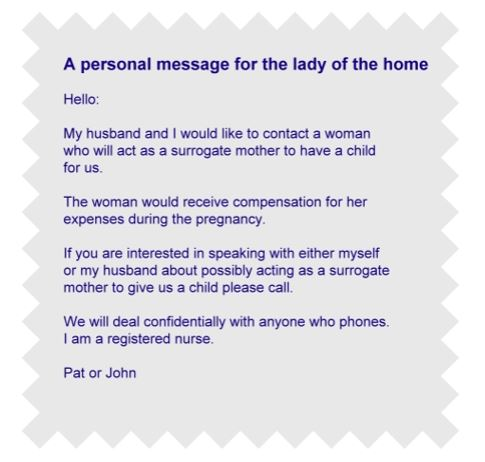
\includegraphics{assets/unit_3/U3_T1_LearningACtivitity.JPG}

\emph{Image showing an example of surrogacy message}

(\emph{You may also wish to consider how the ``Designer Babies'' topic connects to this activity as well.})

\begin{itemize}
\tightlist
\item
  \textbf{\emph{How do you feel about this request?}}
\item
  \textbf{\emph{What problems might you anticipate?}}
\end{itemize}

\emph{Be prepared to share your thoughts with other members of the class}
\end{reflect}

\section{Infancy and Childhood}\label{infancy-and-childhood}

\subsection*{A Child's View of God}\label{a-childs-view-of-god}
\addcontentsline{toc}{subsection}{A Child's View of God}

``One evening on a camping trip several years ago, my wife and I listened outside the tent as our five-year-old Joelle and three-year-old Matthew tried to get to sleep. Always the ``mother,'' Joelle attempted to dispel her little brother's fear of bears and other wild creatures by reminding him that Jesus was watching over them. Not content with generalities, Matt responded, ``Does Jesus got a gun?'''' \emph{(Psychology and Christianity by Ronald Philipchalk, p.~141)}

As any Sunday School teacher knows, children see God differently from adults---often in very concrete terms (protection requires a gun!). Studying cognitive development can help us to understand as well as teach children at their own level.

\subsection*{The Process of Cognitive Change}\label{the-process-of-cognitive-change}
\addcontentsline{toc}{subsection}{The Process of Cognitive Change}

Our textbook provides a good summary of the structure (stages) of cognitive development. The section, however, does not address the process by which a person moves from one stage to the next. Piaget believed that the key to cognitive development is something called cognitive conflict or cognitive disequilibrium. For cognitive development to proceed, the individual must constantly re-evaluate his or her schemas. According to Piaget, we develop schemas from an early age of life. Schemas are our cognitive representations of the world. Schemas help us to organize our experiences. They also allow us to make predictions about what outcomes might result from particular behaviours. Schemas are very important in helping us to understand and to adapt to the world.

Although schemas are important in helping us to understand the world, they are not always accurate. People at all ages can have mental representations of the world that are not correct.

\textbf{\emph{Can you think of any examples of inaccurate schemas?}}

Although people at all ages can have inaccurate mental representations of the world, children are especially prone to view the world in an incorrect way. The reason children may view the world in an incorrect way is because the structure of their cognitive processing is developing. Piaget believed that inaccurate schemas are changed only when they are challenged in the cognitive structure of the child. This challenge has been termed cognitive conflict.

Basically, the process of cognitive change works as follows:

\begin{itemize}
\tightlist
\item
  People are motivated to maintain a state of cognitive equilibrium.\\
\item
  When a child encounters information from the world and the information is inconsistent with his or her schema, the new piece of information creates a state of disequilibrium or cognitive conflict.\\
\item
  \textbf{\emph{Equilibrium}} may be restored through one of the two processes of adapation called assimilation and accommodation.\\
\item
  \textbf{\emph{Assimilation}} occurs when a child re-organizes the new information in such a way as to make the new piece of information consistent with his or her preexisting schema of the world.\\
\item
  \textbf{\emph{Accommodation}} occurs when a child alters his or her schema such that the new piece of information can now be incorporated into the new schema.
\end{itemize}

Thus the process of accommodation produces the greatest cognitive change. Can you think of examples of both assimilation and accommodation? Here is an example:

\textbf{Equilibrium-Preexisting Schema:} Child has grown up in an environment where all people he interacted with were of the same race (mom, dad, siblings, grandma, grandpa, etc.) Child has seen people of other racial groups, but has never interacted with them. Child develops the schema that people tend to like others who are of the same race as him or her.

\textbf{Cognitive Conflict Produced:} At four years of age the child begins to attend preschool. At this time he starts to interact with children of various races. The child begins to develop a friendship with a child of a different race. This friendship creates cognitive conflict for the child: ``How can I like someone who is a different color?'' To resolve this cognitive conflict, the child has two options:

\textbf{\emph{Option A}}- \textbf{Assimilation:} In order to maintain his or her preexisting schema, the child re-organizes the information such that the other child is not perceived to be so dissimilar after all: ``Maybe he is a different color from me, but we both speak English. We must not be so dissimilar after all.''

\textbf{\emph{Option B}}- \textbf{Accommodation:} The child's preexisting schema is altered such that the new information can be incorporated into a new way of perceiving the world, ``Maybe I can be friends with someone who is different from me.''

\subsection*{Cognitive Equilibrium is Restored}\label{cognitive-equilibrium-is-restored}
\addcontentsline{toc}{subsection}{Cognitive Equilibrium is Restored}

Although cognitive equilibrium is restored via either assimilation or accommodation, assimilation serves to maintain an inaccurate schema (that differences inhibit the development of friendships) whereas accommodation serves to produce cognitive change and hence produces a more accurate representation of the world (that differences do not inhibit the development of friendships).

\subsection*{Activity:Cognitive Change}\label{activitycognitive-change}
\addcontentsline{toc}{subsection}{Activity:Cognitive Change}

\begin{reflect}
The first three links below are articles that are intended to give you an opportunity to reflect upon your own considerations around development. The last link is a test - along with the first three links, it is intended to provide some insights about your developmental trajectory in light of your crisis resolution, attachment style, and parenting styles:

\begin{itemize}
\tightlist
\item
  \href{http://www.childdevelopmentinfo.com/development/erickson.shtml}{\textbf{Erik Erikson's Stages of Social-Emotional Development}}\\
\item
  \href{https://www.helpguide.org/articles/childhood-issues/attachment-issues-in-children.htm}{\textbf{Attachment Issues in Children: Causes, Symptoms, Treatment}}\\
\item
  \href{https://www.gottman.com/blog/seven-tips-for-stepfamily-success/}{\textbf{Seven Tips for Stepfamily Success}}
\item
  \href{https://www.3smartcubes.com/pages/tests/parentingstyle/parentingstyle_instructions/}{\textbf{What is Your Parenting Style}}
\end{itemize}
\end{reflect}

\subsection*{Activity: Questions for Consideration}\label{activity-questions-for-consideration-4}
\addcontentsline{toc}{subsection}{Activity: Questions for Consideration}

\begin{reflect}
Before moving on, take a moment to consider the following questions:

\begin{itemize}
\tightlist
\item
  \textbf{\emph{What is God like for children of different levels of cognitive development? If you can, give some examples from children you know\ldots.}}\\
\item
  \textbf{\emph{Would children even have an idea of God if they were not taught it?}}
\end{itemize}

\emph{Be prepared to share your thoughts with other members of the class}
\end{reflect}

\section{Adolescence}\label{adolescence}

John has just turned 13. Over the past year he has experienced may changes. He has grown over six inches and he has developed acne over his face and back. Not only is he changing physically, he is also experiencing a wave of emotional, spiritual, cognitive, and sexual changes. John has become self-focused and very self-critical. In addition, he is beginning to think abstractly and to challenge adults' ``dominion'' on knowledge. John is also on a quest to understand ``who he is'' and ``what his place is in the world''. John's quest for an identity makes him more vulnerable to peer pressure and to the influence of radical groups and cults. During this time that we call adolescence, John will make many decisions that will have a profound effect on the direction his life will take.

\emph{Does any of the above sound familiar?}

Before you begin reading the textbook section on adolescence, think back to your own adolescence. As you think about your experience of adolescence, use the following questions to guide your reflection:

\begin{itemize}
\tightlist
\item
  What physical changes did you experience in adolescence?\\
\item
  How did these physical changes make you feel?\\
\item
  In what ways did your view of the world change during adolescence?\\
\item
  How did your way of treating other people change during adolescence?\\
\item
  What was most important to you during adolescence?\\
\item
  To what extent is ``who you are today'' a function of ``who you became during adolescence''?
\end{itemize}

\subsection*{No Adolescence?}\label{no-adolescence}
\addcontentsline{toc}{subsection}{No Adolescence?}

In other times and in other cultures to­day, adolescence does not exist as a significant and distinct period of develop­ment. This might seem surprising and difficult to imagine. Think of how modern society would be different, or if it could even exist, without a period of adolescence. What are the advantages and disadvantages of having an adolescent period?

\subsection*{Identity}\label{identity}
\addcontentsline{toc}{subsection}{Identity}

The concept of identity is a rich topic for consideration. The most familiar aspect of identity is occupational identity, since much of ``who we are'' in our society rests on the kind of work we do. Perhaps you can readily relate to this in your choice of major. Less familiar, but equally important, is ideological identity. Ideologi­cal identity, including both religious and political orientations, may un­dergo a tremen­dous upheaval during your student years. Do you have the same political beliefs as your parents? What about religious beliefs? Conflict and questioning of parental beliefs and values may be a necessary part of establishing your personal iden­tity---even if the beliefs and values you ultimately adopt are the same as those of your parents.

\subsection*{Activity: Read and Reflect}\label{activity-read-and-reflect}
\addcontentsline{toc}{subsection}{Activity: Read and Reflect}

\begin{reflect}
In this section we explore adolescence and the changes in development we go through. Below are some resources that help to help support your understanding - consider how they connect to the content examined above:

\begin{itemize}
\tightlist
\item
  \href{https://www.sciencedirect.com/journal/journal-of-adolescence}{\textbf{Journal of Adolescence}}\\
\item
  \href{https://childdevelopmentinfo.com/child-development/erickson/\#gs.d8mpcv}{\textbf{Erik Erikson's Stages of Social-Emotional Development}}\\
\item
  \href{https://axis.org/}{\textbf{Connecting Parents, Teens, \& Jesus in a Disconnected World}}
\end{itemize}
\end{reflect}

\subsection*{Activity: Chapter 10 Terminology Practice}\label{activity-chapter-10-terminology-practice}
\addcontentsline{toc}{subsection}{Activity: Chapter 10 Terminology Practice}

\begin{reflect}
In order to review some of the major terms from Chapter 10 in your textbook, practice using the activity below. Although you will not be evaluated on these terms, they will assist you in the assessments for this course:
\end{reflect}

\subsection*{Activity: Question for Consideration}\label{activity-question-for-consideration-1}
\addcontentsline{toc}{subsection}{Activity: Question for Consideration}

\begin{reflect}
Consider what you have learned in this section and take a moment to reflect on the following question:

\begin{itemize}
\tightlist
\item
  \textbf{\emph{Would you want to live your adolescence over again if you could? Why or why not?}}
\end{itemize}

\emph{Be prepared to share your thoughts and insights with other members of the class.}
\end{reflect}

\section*{Assessment}\label{assessment-2}
\addcontentsline{toc}{section}{Assessment}

\begin{assessment}
Refer to the course schedule for graded assignments you are responsible for submitting. \textbf{All graded assignments, and their due dates, can be found on the ``Assessment'' tab.}

In addition to any graded assignments you are responsible for submitting, be sure to complete all the Learning Activities that have been provided throughout the content - these are intended to support your understanding of the content.
\end{assessment}

\section*{Checking your Learning}\label{checking-your-learning-2}
\addcontentsline{toc}{section}{Checking your Learning}

\begin{progress}
Before you move on to the next unit, check that you are able to:

\begin{itemize}
\tightlist
\item
  Define the key terminology related to prenatal and infant physical development, infancy and childhood, and adolescent development.\\
\item
  Understand advantages and disadvantages to different research designs in developmental psychology.\\
\item
  Understand the cognitive changes that occur during infancy and childhood, and the importance of attachment and the different styles of attachment.\\
\item
  Understand the process of identity formation, relationships, and moral emotions during adolescence.\\
\item
  Apply your understanding to identify the best ways expectant parents can ensure the health of their developing fetus, how to promote learning, and how to categorize moral reasoning.\\
\item
  Analyze the effects of preterm birth, how to effectively discipline children, and adolescent judgment and risk taking.
\end{itemize}
\end{progress}

\chapter{The Developing Person - Part 2}\label{the-developing-person---part-2}

\section*{Overview}\label{overview-3}
\addcontentsline{toc}{section}{Overview}

Building upon Unit 3, this unit (Part 2) will focus on the cognitive, physical, and social changes faced during young (and emerging) adulthood, middle adulthood, and late adulthood.

\emph{Please note - although it is not covered in the text, Topic 2 discusses the important, and inevitable, subject of dying and death.}

\subsection*{Topics}\label{topics-3}
\addcontentsline{toc}{subsection}{Topics}

This unit is divided into the following topics:

\begin{enumerate}
\def\labelenumi{\arabic{enumi}.}
\tightlist
\item
  Adulthood\\
\item
  Death and Dying
\end{enumerate}

\subsection*{Learning Outcomes}\label{learning-outcomes-3}
\addcontentsline{toc}{subsection}{Learning Outcomes}

By the end of this unit, student's will be able to:

\begin{itemize}
\tightlist
\item
  Define the key terminology concerning adulthood and aging.\\
\item
  Describe the key areas of growth experiences by emerging adults.
\item
  Explain age-related disorders such as Alzheimer's disease.\\
\item
  Describe how cognitive abilities change with age.\\
\item
  Apply effective communication principles to the challenge of improving your own relationships.\\
\item
  Analyze the stereotype that old age is a time of unhappiness.
\end{itemize}

\subsection*{Activity Checklist:}\label{activity-checklist-3}
\addcontentsline{toc}{subsection}{Activity Checklist:}

Here is a checklist of learning activities you will benefit from in completing this unit. You may find it useful for planning your work.

\begin{reflect}
{Learning Activities}

\begin{itemize}
\tightlist
\item
  Read the relevant sections of Chapter 10 of your textbook
\item
  Review the Chapter 10 - Notes (intended to support your understanding of your readings)
\item
  Read about \emph{Erikson's Eight Psychosocial Stages} that highlight the importance of relationships in healthy aging.
\item
  Read and Reflect: Explore the resources that focus on again and dying and consider how these concepts affect individuals.
\end{itemize}
\end{reflect}

\begin{caution}
\textbf{\emph{Note}}

The course units follow topics in the textbook, \emph{Revel for An Introduction to Psychological Science} by Krause et al.~(4th Edition). For each unit, please read the pertinent chapter(s) before completing the assessment for the unit.
\end{caution}

\begin{assessment}
\textbf{\emph{Assessment}}

In this course you demonstrate your understanding of the course learning outcomes in different ways, including papers, projects, discussions and quizzes. Please see the Assessment section in Moodle for assignment details and due dates.
\end{assessment}

\subsection*{Resources}\label{resources-3}
\addcontentsline{toc}{subsection}{Resources}

Here are the resources you will need to complete this unit:

\begin{itemize}
\tightlist
\item
  Krause, M., Corts, D., \& Smith, S. C. (2024). \emph{Revel for An Introduction to Psychological Science, 4th Canadian Edition.} Pearson Ed.
\item
  Other resources will be provided online.
\end{itemize}

\section{Adulthood}\label{adulthood}

\subsection*{Psychosocial Development}\label{psychosocial-development}
\addcontentsline{toc}{subsection}{Psychosocial Development}

There are many changes we experience during the time we call adulthood. According to Erikson's theory of psychosocial development, adults move through three important stages during which they must resolve important psychosocial conflicts:

\begin{itemize}
\tightlist
\item
  Early Adulthood\\
\item
  Middle Adulthood\\
\item
  Late Adulthood
\end{itemize}

\textbf{\emph{In Early Adulthood}} (20-40 years of age) the psychosocial crisis is one of intimacy versus isolation. Although it is often perceived as critical whether or not the person develops an intimate relationship with a lifelong partner, Erikson believed that although this is one component of intimacy in this stage, other types of intimacy are also important---like developing intimate relationships with workmates, colleagues, and even one's children. If one fails to develop a sense of intimacy during this stage, he or she will feel isolation.

\textbf{\emph{In Middle Adulthood}} (40-65 years of age) the psychosocial crises is one of generativity versus stagnation. What is generativity? Erikson used the term gererativity to describe the process by which a person feels like he or she is making a lasting contribution in the world. Usually, generativity involves giving something back to the next generation. People at this stage can feel generative in many ways---coaching a softball team, being a scout leader, teaching children in Sunday School, been a big brother/sister, etc. If a person fails to develop a sense of generativity during this stage, he or she will feel a sense of stagnation.

\textbf{\emph{In Late Adulthood}} (65+ years of age) the psychosocial crisis is one of ego integrity versus despair. If the individual looks back on his or her life and feels a sense of pride in the accomplishments he or she has made, then the individual will feel a sense of ego integrity. However, if the person looks back on his or her life and does not see the significance of his or her accomplishments, then he or she will feel a sense of despair at the meaninglessness of his or her life.

\subsection*{Guilt}\label{guilt}
\addcontentsline{toc}{subsection}{Guilt}

One of the most significant developments in childhood, from both a secular and Christian point of view, is a conscience with its attendant guilt. Is guilt simply a conditioned emotional response (as the behaviorist might say)? Is it the result of conflict with the superego (as a psychoanalyst would say)? Is it the failure to live up to our self-concept (as the humanist might say)? Is it the voice of the Holy Spirit? Or is it some combination of these? (For help on this issue and an important distinction between false and true guilt see Counts and Narramore (1970), Narramore (1984), Tournier (1962).) \emph{(from Psychology and Christianity, by Ronald Philipchalk, p.~146)}

The textbook discusses moral development in childhood and adolescence. However, many adults are troubled by questions of right and wrong, and in particular, by feelings of guilt. The Christian authors noted above suggest that many guilt feelings are not true guilt but false guilt carried over from childhood experiences. Understanding how conscience and guilt feelings develop can help to liberate us from unnecessary false guilt inappropriately attributed to God.

\subsection*{Activity: Read and Reflect}\label{activity-read-and-reflect-1}
\addcontentsline{toc}{subsection}{Activity: Read and Reflect}

\begin{reflect}
This activity involves some reading and reflection around Erikson's Eight Psychosocial Stages and an article from Harvard University illuminating the importance of relationships in healthy aging.

\begin{itemize}
\tightlist
\item
  \href{https://childdevelopmentinfo.com/child-development/erickson/\#gs.d8mpcv}{\textbf{Erik Erikson's Stages of Social-Emotional Development}}\\
\item
  \href{https://news.harvard.edu/gazette/story/2017/04/over-nearly-80-years-harvard-study-has-been-showing-how-to-live-a-healthy-and-happy-life/}{\textbf{Good Genes are Nice, but Joy is Better}}
\end{itemize}
\end{reflect}

\subsection*{Activity: Questions for Consideration}\label{activity-questions-for-consideration-5}
\addcontentsline{toc}{subsection}{Activity: Questions for Consideration}

\begin{reflect}
Take some time to consider what you have learned in this section. Think about the following questions:

\begin{itemize}
\tightlist
\item
  \textbf{\emph{What do you hope to accomplish during your ``adult development'' years?}}

  \begin{itemize}
  \tightlist
  \item
    \emph{(If you are past these years, what are you most pleased with?)}
  \end{itemize}
\end{itemize}

\emph{Be prepared to share your thoughts with other members of the class}
\end{reflect}

\section{Death and Dying}\label{death-and-dying}

\subsection*{Death}\label{death}
\addcontentsline{toc}{subsection}{Death}

Secular psychologists see death as final. Christians, however, see resurrection beyond, with death being but another step in that direction. What implications do these beliefs have for the process of dying?

As medical technology has advanced death has become more and more difficult to define. We need to focus our attention less on preserving the physical and more on preserving the personhood of the individual. This means giving greater attention to our concept of the dying person created in the image of God (as the abortion issue has forced us to do at the other end of life). When is personhood sacrificed to technical efficiency? Should we advocate a more ``natural death?'' What is ``natural death?'' How far does one go in ``allowing'' natural death? \emph{(from Psychology and Christianity, by Ronald Philipchalk, p.~146)}

\subsection*{Hospice}\label{hospice}
\addcontentsline{toc}{subsection}{Hospice}

``You matter because of who you are. You matter to the last moment of your life, and we will do all we can not only to help you die peacefully, but also to live until you die.'' \emph{(Dame Cicely Saunders)}

During the Crusades of the Middle Ages a hospice provided lodging for travelers: a place of refuge and comfort. So in 1967, when Dame Cicley Saunders opened a facility in London to provide care and comfort to dying people and their families, St.~Christopher's hospice was an appropriate name. \emph{(Courtesy of the Langley Hospice Society)}

\emph{If you would like to know more about the hospice movement in this area, you can contact the Langley Hospice Society at 604-530-1115.}

\subsection*{Cultural Variations}\label{cultural-variations}
\addcontentsline{toc}{subsection}{Cultural Variations}

The following issues are often subject to cul­tural variations:

\begin{itemize}
\tightlist
\item
  Adolescence is unknown in some cultures\\
\item
  Adolescent struggles and conflict are much less in some cultures (e.g., )\\
\item
  Stage theories may not apply in other cultures\\
\item
  Ageism, especially with regard to intellectual abilities, is reduced, unknown, or even reversed in some cultures where the wisdom of old age is venerated\\
\item
  The ``social clock'' may be set differently in other cultures\\
\item
  Attitudes toward death vary greatly between cultures
\end{itemize}

\section{Assessment}\label{assessment-3}

\begin{assessment}
Refer to the course schedule for graded assignments you are responsible for submitting. \textbf{All graded assignments, and their due dates, can be found on the ``Assessment'' tab.}

In addition to any graded assignments you are responsible for submitting, be sure to complete all the Learning Activities that have been provided throughout the content - these are intended to support your understanding of the content.
\end{assessment}

\section*{Checking your Learning}\label{checking-your-learning-3}
\addcontentsline{toc}{section}{Checking your Learning}

\begin{progress}
Before you move on to the next unit, check that you are able to:

\begin{itemize}
\item
  Define the key terminology concerning adulthood and aging.
\item
  Describe the key areas of growth experiences by emerging adults.
\item
  Explain age-related disorders such as Alzheimer's disease.
\item
  Describe how cognitive abilities change with age.
\item
  Apply effective communication principles to the challenge of improving your own relationships.
\item
  Analyze the stereotype that old age is a time of unhappiness.
\end{itemize}
\end{progress}

\chapter{Personality}\label{personality}

\section*{Overview}\label{overview-4}
\addcontentsline{toc}{section}{Overview}

In Unit 5 of the course, our attention will focus on personality. The study of personality attempts to answer the questions: \emph{Who are you?} and, \emph{How did you become who you are?} As human's are astoundingly complex, there is not any one theory that can capture, in totality, a description of who you are; hence, there are numerous approaches and theories that attempt to address these questions. In this unit, you will learn about some of the contemporary approaches to the study of Personality, and examine and review cultural, biological, Psychodynamic and Humanistic approaches to Personality.

\subsection*{Topics}\label{topics-4}
\addcontentsline{toc}{subsection}{Topics}

This unit is divided into the following topics:

\begin{enumerate}
\def\labelenumi{\arabic{enumi}.}
\tightlist
\item
  Psychoanalytic View\\
\item
  Humanistic View\\
\item
  Trait View\\
\item
  Social-Cognitive View
\end{enumerate}

\subsection*{Learning Outcomes}\label{learning-outcomes-4}
\addcontentsline{toc}{subsection}{Learning Outcomes}

By the end of this unit, student's will be able to:

\begin{itemize}
\tightlist
\item
  Define the key terminology associated with contemporary approaches, cultural and biological approaches, and psychodynamic and humanistic approaches to personality.\\
\item
  Describe the behaviourist and social-cognitive views, evolutionary theories, and Freudian developmental and defensive explanations of personality.\\
\item
  Apply the ``Big Five'' personality traits, psychodynamic, and humanistic perspectives to understand personality.\\
\item
  Analyze the roots of violence and prejudice, roles of personality traits and psychological and physical states, and the genetic basis of personality in determining behaviour.\\
\item
  Assess claims that males and females have fundamentally different personalities and whether projective tests are valid measures of personality.
\end{itemize}

\subsection*{Activity Checklist:}\label{activity-checklist-4}
\addcontentsline{toc}{subsection}{Activity Checklist:}

Here is a checklist of learning activities you will benefit from in completing this unit. You may find it useful for planning your work.

\begin{reflect}
{Learning Activities}

\begin{itemize}
\tightlist
\item
  Read the relevant sections of Chapter 12 of your textbook
\item
  Review the Chapter 12 - Notes (intended to support your understanding of your readings)
\item
  Read about a \emph{Christian Perspective on Dreams}
\item
  Read and Reflect: \emph{Birth Order and Your Personality}
\item
  Explore the three resources on self-esteem and humanistic psychology
\item
  Explore the \emph{Queendom} personality resource and take a personality test (ungraded)
\item
  Read and reflect upon the resources focused on sense of agency
\item
  Complete the Key Terms Quiz for Unit 5 (ungraded)
\end{itemize}
\end{reflect}

\begin{caution}
\textbf{\emph{Note}}\\
The course units follow topics in the textbook, \emph{Revel for An Introduction to Psychological Science} by Krause et al.~(4th Edition). For each unit, please read the pertinent chapter(s) before completing the assessment for the unit.
\end{caution}

\begin{assessment}
\textbf{\emph{Assessment}}\\
In this course you demonstrate your understanding of the course learning outcomes in different ways, including papers, projects, discussions and quizzes. Please see the Assessment section in Moodle for assignment details and due dates.
\end{assessment}

\subsection*{Resources}\label{resources-4}
\addcontentsline{toc}{subsection}{Resources}

Here are some additional resources that will help you complete this unit:

\begin{itemize}
\tightlist
\item
  Krause, M., Corts, D., \& Smith, S. C. (2024). \emph{Revel for An Introduction to Psychological Science, 4th Canadian Edition.} Pearson Ed.
\item
  Other resources will be provided online.
\end{itemize}

\section{Psychoanalytic View}\label{psychoanalytic-view}

``We are sent into this world to acquire a personality and a character to take with us that can never be taken from us.'' \emph{(In a letter from a WW II Royal Air Force pilot to his mother)}

\subsection*{Personality Theories}\label{personality-theories}
\addcontentsline{toc}{subsection}{Personality Theories}

In this chapter we consider the topic of personality theories. In doing this we examine several major perspectives. Within each of these there are many variations (e.g., Adler, Jung, and Freud within the psychoanalytic perspective). If you would like to know more about this area, you might be interested in taking the course ``Theories of Personality'' \emph{(Psychology 301 at TWU).}

Aside from all these more formal theories, each of us has an implicit personality theory. This is our personal idea of what people are like, including which personality characteristics go together. For example, we think of people who are attractive and intelligent as likable rather than unlikable. Our socialization leads us to assume certain traits go together. As you go through this chapter, you may find some approaches are closer to your own assumptions (implicit theory), and you may prefer these approaches to others. You may also find your implicit theory becomes more explicit. Finally, you may even modify your own theory in the face of new information.

\subsection*{Dreams}\label{dreams}
\addcontentsline{toc}{subsection}{Dreams}

``And afterward, I will pour out my Spirit on all people. Your sons and daughters will prophesy, your old men will dream dreams, your young men will see visions'' \emph{(Joel 2:28)}.

God apparently spoke through dreams many times in the bible, and in Joel 2:28 He promised to do so in the future. Does God still (or again) speak through dreams? Are we missing out on a possible leading from God when we ignore our dreams? If you would like to read more on this subject you might be interested in books by Christians on this subject. For example, see John A. Sanford's Dreams, God's Forgotten Language, or Morton T. Kelsey's God, Dreams, and Revelation, or Abraham Schmitt's Before I Wake. The website below (cf.~Online Resources) contains some balanced advice. Also, voice your opinion or give your experience in the online discussion.

\subsection*{Birth Order}\label{birth-order}
\addcontentsline{toc}{subsection}{Birth Order}

You may be familiar with Adler's concept of the family constellation, which implies that position in the family has a powerful effect on goals, self-concept, and ways of relating to others.

As a test of this concept, think of a three-child family, all of whom were born within a few years (using larger families makes things too complicated). Try applying Adler's theory to predict which child in the family is likely to be:

\begin{itemize}
\tightlist
\item
  the best student\\
\item
  the most shy\\
\item
  the most helpful around the house\\
\item
  the most outgoing\\
\item
  the ``hell raiser''\\
\item
  the most ``helpless''\\
\item
  the charmer\\
\item
  the ``baby'' of the family
\end{itemize}

You will not always be right---but neither was Adler. The important thing is to note that Adler made psychology aware of the different expectations and social influences on different children in the same family. In some respects, children in the same position in different families are more alike than are children in differ­ent positions in the same family

\subsection*{Activity: Read and Reflect}\label{activity-read-and-reflect-2}
\addcontentsline{toc}{subsection}{Activity: Read and Reflect}

\begin{reflect}
Having just introduced Personality Theories to the course, we begin to explore psychoanalytic views of human development. Dreams and birth order are but two of the constructs that help shape and reflect who we are as individuals- there are many different theories and interpretations on the role dreams and birth order play. Take a moment to consider the following articles:

\begin{itemize}
\tightlist
\item
  \href{https://www.cgg.org/index.cfm/fuseaction/Library.sr/CT/BQA/k/96/What-Is-Proper-Christian-Perspective-on-Dreams-Visions.htm}{\textbf{Christian Perspective on Dreams}}\\
\item
  \href{https://www.scientificamerican.com/article/ruled-by-birth-order/}{\textbf{Birth Order and Your Personality}}
\end{itemize}
\end{reflect}

\subsection*{Activity: Questions for Consideration}\label{activity-questions-for-consideration-6}
\addcontentsline{toc}{subsection}{Activity: Questions for Consideration}

\begin{reflect}
Take a moment to reflect on what you have learned in this section. Use the following questions to guide your self-reflection:

\begin{itemize}
\tightlist
\item
  \textbf{\emph{Does God speak through dreams?}}\\
\item
  \textbf{\emph{What reasons do you have for your opinion? Can you give an example?}}
\end{itemize}

\emph{Be prepared to share your thoughts and insights with other members of the class.}
\end{reflect}

\section{Humanistic View}\label{humanistic-view}

\subsection*{Self-Esteem}\label{self-esteem}
\addcontentsline{toc}{subsection}{Self-Esteem}

In 1890, William James gave a simple formula for self-esteem:

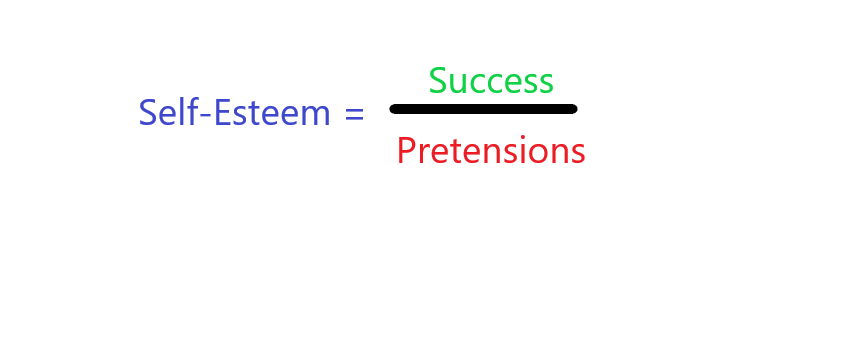
\includegraphics{assets/unit_5/Unit5_Topic2_Image.png}

\emph{James explained:}

Such a fraction may be increased as well by diminishing the denominator as by increasing the numerator. To give up pretensions is as blessed a relief as to get them gratified; and where disappointment is incessant and the struggle unending, this is what men will always do. . . . How pleasant is the day we give up striving to be young---or slenderThank Godwe say, those illusions are gone. \emph{(James, 1890) (Quoted from Invitation to Social Psychology by Ron Philipchalk)}

\subsection*{Self-Esteem: A Contrary View}\label{self-esteem-a-contrary-view}
\addcontentsline{toc}{subsection}{Self-Esteem: A Contrary View}

Self-esteem is a popular topic in North American society and researchers have expended a vast amount of effort studying it. Approximately 10,000 studies have explored the possible relationship between self-esteem and various human problems (Scheff et al., 1989). The assumption that low self-esteem is at the root of many personal and social problems has reached the level of a cultural truism. The California legislature (1990) has even established a task force to promote self-esteem, believing that enhanced self-esteem is a vaccine against drug abuse, teen-age pregnancy, welfare dependency, and other social ills. Sharon Neuman (1992) suggests that the need to enhance self-esteem has become a ``motherhood issue''---meaning that belief in its value is so widely accepted it goes unquestioned.

Recently, however, several authors have begun to challenge this focus on raising self-esteem. They point out that high self-esteem can sometimes be detrimental, if, for example, it leads people to set inappropriate, risky goals that are beyond their capabilities (Baumeister, et al., 1993a). In addition, the relationship between self-esteem and other measures of well-being is often weak or nonexistent (Burr \& Christensen, 1992; Hermans, 1992; Jackson, 1984). Perhaps most importantly, high self-esteem may be the result and not the cause of other positive tendencies (Alexander \& Baker, 1992).

Sharon Neuman (1992) argues that self-esteem must follow, not precede, real achievement. She claims that no number of self-esteem programs can replace the genuine satisfaction of a job well done. Wesley Burr and Clark Christensen (1992) suggest that the idea that we must esteem ourselves highly before we can value and love others is a ``Western myth.'' They add:

We would improve our thinking if we were to take the idea that ``we cannot love others until we love ourself'' and turn it 180 degrees to be: ``We cannot love ourself until we love others.'' We would further improve our thinking if we then concluded that this is a fairly irrelevant and unimportant idea anyway because it still implies that loving ourself is what is important. (p.~464)

Burr and Christensen suggest that self-esteem is a fruit and not a root of healthy emotional connections between people. \emph{(From Invitation to Social Psychology by Ron Philipchalk)}

\section{Christianity \& Humanism}\label{christianity-humanism}

Some Christians object to the humanistic perspective because of its unqualified affirmation of human goodness and its apparent promotion of self-love. It is important to note, however, that humanistic psychology is not to be equated with the philosophy and social movement called humanism. Although it focuses on humans, so too do other approaches to personality. (The behavioral psychologist B.F. Skinner was a signatory to the Humanist Manifesto but a major opponent of humanistic psychology.) In his authoritative work on the history of psychology, Ernest Hilgard writes, ``Humanistic psychology as something contemporary is not to be confused with other forms of humanism, such as humanistic studies which refer to classical or liberal arts topics, or that form of humanism which sets itself against theological beliefs (1987, p.~504). In fact, J.I. Packer and Thomas Howard in their book Christianity: The true humanism (1985) argue that only Christianity gives a valid basis for assuming humans have value.

\subsection*{Activity: Read and Reflect}\label{activity-read-and-reflect-3}
\addcontentsline{toc}{subsection}{Activity: Read and Reflect}

\begin{reflect}
As we explore a humanistic view, as it relates to personality, we start to see the development of self-esteem. Take some time to read through the following resources and consider how they connect to what you have learned:

\begin{itemize}
\tightlist
\item
  \href{http://healthyselfesteem.org/}{\textbf{National Association for Self-Esteem}}\\
\item
  \href{https://www.apa.org/about/division/div32}{\textbf{Society for Humanistic Psychology}}
\end{itemize}

\emph{The purpose of these resources is to help you assess your self-esteem, help to build a healthy self-esteem, and to provide you with a credible site for learning more about Humanistic Psychology.}
\end{reflect}

\subsection*{Activity: Question for Consideration}\label{activity-question-for-consideration-2}
\addcontentsline{toc}{subsection}{Activity: Question for Consideration}

\begin{reflect}
Consider the following question - think about how it connects to what you have learned in this section:

\begin{itemize}
\tightlist
\item
  \textbf{\emph{If you wanted to study the psychologically healthiest individuals, whom would you study? How would you decide?}}
\end{itemize}

\emph{Be prepared to share your thoughts with other members of the class}
\end{reflect}

\section{Trait View}\label{trait-view}

\subsection*{Trait Theory}\label{trait-theory}
\addcontentsline{toc}{subsection}{Trait Theory}

In the previous lesson we discussed implicit theories of personality. Many people's implicit theories include elements of trait theory. They believe that personality is made up of traits. For example, popular ideas of leadership and success often rest on this assumption (e.g., Traits for success).

Actually this view is quite old, going back to the ancient Greeks:

Almost 2,000 years ago a Greek physician named Galen suggested that there were four basic types of personality, based on four different ``humors,'' or fluids, in the body. Galen called these personality types sanguine, phlegmatic, choleric, and melancholic. When Eysenck combined his two basic personality scales, he found that he had a ``less humorous'' version of a classic theory. \emph{(from Understanding Human Behavior by Ron Philipchalk \& James McConnell)}

In psychology today there is a growing effort towards accurate measurement of personality traits, and investigation of the ways in which traits interact with the environment.

One of the most popular applications of trait theory is in the prediction of employee success. After looking at the ``Big 5,'' which trait do you think is the most important? Imagine you own a business and you have to make a quick decision to hire one of 5 very similar applicants. The only trait measure you have is each applicant's score on the ``Big 5.'' The only problem is that each one scores high on a different factor. Which one would you hire?

\subsection*{Measuring Personality}\label{measuring-personality}
\addcontentsline{toc}{subsection}{Measuring Personality}

The trait approach to personality is closely linked to the matter of psychological testing. The strength of this approach is that it provides quantifiable data for analysis and comparison. The weakness is the difficulty in measuring traits accurately. Remember our discussion of \emph{standardization, validity,} and \emph{reliability} of intelligence tests? Personality tests must also meet the same criteria. (An additional problem is that our situations guide us as well as our traits.) This is an important point to remember when you encounter the many so-called personality tests in the popular media.

\subsection*{Barnum Effect}\label{barnum-effect}
\addcontentsline{toc}{subsection}{Barnum Effect}

Do you have a desire to know what ``kind'' of person you are? This common desire can be used to manipulate you in a variety of ways. As discussed in the textbook, sometimes it is easier to make people believe that you are measuring their personality than it is to actually measure it. In fact, it is remarkably easy for people to be convinced that a personality profile describes them well. This phenomena is known as ``the Barnum effect,'' after the circus showman P. T. Barnum. The Barnum effect hearkens back to the late 1940s, when psychologist Bertram Forer gave research participants a personality test and then generated a personality description that subjects believed was based on their test responses. Even though all participants were given exactly the same personality description, they found the profile to be highly convincing and descriptive of them as an individual. When asked to rate how well the profile described them, on a scale ranging from 0 (very poor) to 5 (excellent), the average rating was an impressive 4.26 (Forer, 1949)You, too, can try this experiment. Read the personality description below and rate, on a scale ranging from 0 (very poor) to 5 (excellent), how well this description describes you:

\emph{You have a strong need for other people to like you and for them to ad­mire you. You have a tendency to be critical of yourself. You have a great deal of unused energy which you have not turned to your advantage. While you have personality weaknesses, you are generally able to compensate for them. Your sexual adjustment has presented some problems for you. Dis­ci­plined and controlled on the outside, you tend to be worrisome and in­se­cure inside. At times you have serious doubts as to whether you have made the right decision or done the right thing. You prefer a certain amount of change and variety and become dissatisfied when hemmed-in by restrictions and limitations. You pride yourself as being an independent thinker and do not accept other opinions without satisfactory proof. You have found it un­wise to be too frank in revealing yourself to others. At times you are extro­verted, affable, sociable, while at other times you are introverted, wary, and reserved. Some of your aspirations tend to be pretty unrealistic.}

\subsection*{Activity: Practice, Read, and Reflect}\label{activity-practice-read-and-reflect}
\addcontentsline{toc}{subsection}{Activity: Practice, Read, and Reflect}

\begin{reflect}
In this topic we have continued to develop our understanding of personality. Below are some tests you can take - consider the results and reflect on how useful these types of resources are in assessing personality:

\begin{itemize}
\tightlist
\item
  \href{https://www.queendom.com/}{\textbf{Queendom.com}}
\end{itemize}

\emph{Queendom.com} is a great resource for different kinds of tests. You will be looking specifically at Personality tests on this site. When you go to www.queendom.com, click on the \textbf{\emph{``TESTS, QUIZZES \& POLLS''}} tab and select \textbf{TESTS.} From the \textbf{\emph{PERSONALITY TESTS}} list select ONE of the following personality tests:

\begin{itemize}
\tightlist
\item
  DISC Personality Test\\
\item
  Big Five Personality Test\\
\item
  Self-Control \& Self-Monitoring Test\\
\item
  Happiness Test\\
\item
  Locus Of Control \& Attributional Style Test
\end{itemize}

Interact with the results and ponder whether or not you think the test is accurate or inaccurate and whether or not the information provided seems unique to you or could it be applied to anyone given the right situation.
\end{reflect}

\subsection*{Activity: Question for Consideration}\label{activity-question-for-consideration-3}
\addcontentsline{toc}{subsection}{Activity: Question for Consideration}

\begin{reflect}
Take a moment to reflect on the following question - consider how they connect to what you have learned in this section:

\begin{itemize}
\tightlist
\item
  \textbf{\emph{What is the role of heredity in personality?}}\\
\item
  \textbf{\emph{Is our personality inherited and set for life? Can it be modified?}}
\end{itemize}

Author Tim LaHaye has taken the Greek idea of types and body humors and adapted it to a Christian perspective incorporating the concept of spiritual gifts.

\begin{itemize}
\tightlist
\item
  \textbf{\emph{Does the bible support an approach to personality that links individual differences to inherited traits?}}\\
\item
  \textbf{\emph{What is the role of the Holy Spirit in relationship to traits? - Are these different ``gifts'' (I Cor. 12)? Different ``fruit (Gal 5:22)? Can they be changed?}}
\end{itemize}

\emph{Be prepared to share your thoughts and insights with other members of the class}
\end{reflect}

\section{Social-Cognitive View}\label{social-cognitive-view}

\subsection*{You + Your Environment}\label{you-your-environment}
\addcontentsline{toc}{subsection}{You + Your Environment}

Social-Cognitive Theory (SCT) was originally formulated by Albert Bandura at Stanford University. The fundamental premise of SCT is that models serve as the basis for learning new behaviours and that learning occurs in a social context with a dynamic and reciprocal interaction of the person, environment, and behavior; this is known as reciprocal determinism. Its emphasis is on external and internal social reinforcement and how these factors shape and maintain behavior in different environments. The theory also recognizes the influence of a person's past experiences, which factor into whether behavioral action will occur. These past experiences serve as the primary reinforcements and expectancies, shaping whether or not a person will engage in a specific behavior and answering why a person engages in that behaviour.

In summary, the Social-Cognitive view recognizes the mutual interdependence (``reciprocal determinism'') of individual qualities and situations. While we do have individual patterns of behaviour, we exhibit these according to the way we perceive our situation.

\subsection*{Activity: Read and Reflect}\label{activity-read-and-reflect-4}
\addcontentsline{toc}{subsection}{Activity: Read and Reflect}

\begin{reflect}
Who we are is, in large part, shaped by the environment in which live. Take a moment to consider the following resources and how they relate to this concept:

\begin{itemize}
\tightlist
\item
  \href{http://www.ldonline.org/article/6154/}{\textbf{Learned Helplessness}}\\
\item
  \href{https://nesslabs.com/learned-optimism}{\textbf{Learned Optimism}}
\end{itemize}

The above resources will help you to think about how your environment can impact your sense of agency (the ability to choose your behaviours to impact the environment) and how your sense of agency can influence your environment. This demonstrates the key idea of Social-Cognitive Theory, that you are in a constant, dynamic relationship with your environment and each factor is shaped by the other.
\end{reflect}

\subsection*{Activity: Chapter 12 Key Terms Quiz}\label{activity-chapter-12-key-terms-quiz}
\addcontentsline{toc}{subsection}{Activity: Chapter 12 Key Terms Quiz}

\begin{reflect}
In order to review some of the major terms from Chapter 12 in your textbook, take the following unmarked quiz. Although you will not be evaluated on these terms, they will assist you in the assessments for this course:
\end{reflect}

\subsection*{Activity: Questions for Consideration}\label{activity-questions-for-consideration-7}
\addcontentsline{toc}{subsection}{Activity: Questions for Consideration}

\begin{reflect}
Take a moment to reflect on what you have learned in this section. Read the following statement and consider the questions below:

\emph{Research indicates that an internal locus of control is associated with more positive psychological outcomes than an external locus of control.}

\begin{itemize}
\tightlist
\item
  \textbf{\emph{Does this mean that Christians (and others who believe in God) are less psychologically healthy because they believe an external force (God) is in control?}}
\end{itemize}

*Be prepared to share your thoughts and insights with other members of the class.
\end{reflect}

\section*{Assessment}\label{assessment-4}
\addcontentsline{toc}{section}{Assessment}

\begin{assessment}
Refer to the course schedule for graded assignments you are responsible for submitting. \textbf{All graded assignments, and their due dates, can be found on the ``Assessment'' tab.}

In addition to any graded assignments you are responsible for submitting, be sure to complete all the Learning Activities that have been provided throughout the content - these are intended to support your understanding of the content.
\end{assessment}

\section*{Checking your Learning}\label{checking-your-learning-4}
\addcontentsline{toc}{section}{Checking your Learning}

\begin{progress}
Before you move on to the next unit, check that you are able to:

\begin{itemize}
\tightlist
\item
  Know the key terminology associated with contemporary approaches, cultural and biological approaches, and psychodynamic and humanistic approaches to personality.\\
\item
  Describe the behaviourist and social-cognitive views, evolutionary theories, and Freudian developmental and defensive explanations of personality.\\
\item
  Apply the Big Five personality traits, psychodynamic, and humanistic perspectives to understand personality.\\
\item
  Analyze the roots of violence and prejudice, roles of personality traits and psychological and physical states, and the genetic basis of personality in determining behaviour.\\
\item
  Analyze claims that males and females have fundamentally different personalities and whether projective tests are valid measures of personality.
\end{itemize}
\end{progress}

\chapter{Social Psychology - Part 1}\label{social-psychology---part-1}

\section*{Overview}\label{overview-5}
\addcontentsline{toc}{section}{Overview}

No single factor has more impact on shaping the quality and direction of your life over virtually every aspect of your existence than relationships. In a way, everyone is a social psychologist. People constantly form ideas/opinions about why a person or a group of people are acting the way they are. Social psychology is similar to what people find themselves naturally doing except it uses scientific tools to study these hypotheses (the ideas/opinions). Social psychologist are primarily interested in examining the different ways that individual's effect groups of people and the way groups of people effect individual's. In this unit you will be introduced to some historical studies and main concepts in this field. Topics covered in this chapter include social influences on behaviour, social impressions and judgements, the relationship between attitudes and behaviour, and effective communication. Unit 6 (Part 1) looks at attributes and actions, conformity, obedience, and compliance. Unit 7 (Part 2) examines prejudice and aggression, and, though not specifically covered in the textbook, yet important to social psychology, attraction and altruism.

\subsection*{Topics}\label{topics-5}
\addcontentsline{toc}{subsection}{Topics}

This unit is divided into the following topics:

\begin{enumerate}
\def\labelenumi{\arabic{enumi}.}
\tightlist
\item
  Attributes and Actions\\
\item
  Conformity\\
\item
  Obedience\\
\item
  Compliance
\end{enumerate}

\subsection*{Learning Outcomes}\label{learning-outcomes-5}
\addcontentsline{toc}{subsection}{Learning Outcomes}

By the end of this unit, student's will be able to:

\begin{itemize}
\tightlist
\item
  Define, and apply, the key terminology associated with social influence, social cognition, and on attitudes, behaviour, and effective communication.\\
\item
  Describe why individuals conform to others' behaviours, how individuals and groups can influence behaviours, and how we form first impressions and how these impressions influence us.\\
\item
  Apply your knowledge of the bystander effect to ensure that you will be helped if you are in an emergency, of social cognition to help overcome prejudice and discrimination, and of the central route to describe how a message should be designed.\\
\item
  Analyze whether guards who participate in abuse are inherently bad people, or if their behaviour is the product of social influences and whether people who commit discriminatory acts are necessarily prejudiced.\\
\item
  Describe how behaviours influence attitudes in terms of cognitive dissonance theory.
\end{itemize}

\subsection*{Activity Checklist:}\label{activity-checklist-5}
\addcontentsline{toc}{subsection}{Activity Checklist:}

Here is a checklist of learning activities you will benefit from in completing this unit. You may find it useful for planning your work.

\begin{reflect}
{Learning Activities}

\begin{itemize}
\tightlist
\item
  Read the relevant sections of Chapter 13 of your textbook
\item
  Review the Chapter 13 - Notes (intended to support your understanding of your readings)
\item
  Read about \emph{Attribution Theory} and \emph{Cognitive Dissonance}\\
\item
  Read and Reflect on the two articles \emph{Social Influence} and \emph{Conformity and Obedience}
\item
  Read the four resources on ethical guidelines when performing research
\item
  Explore the two articles on the \emph{Influence of Social Media} and \emph{Cults}
\end{itemize}
\end{reflect}

\begin{caution}
\textbf{\emph{Note}}\\
The course units follow topics in the textbook, \emph{Revel for An Introduction to Psychological Science} by Krause et al.~(4th Edition). For each unit, please read the pertinent chapter(s) before completing the assessment for the unit.
\end{caution}

\begin{assessment}
\textbf{\emph{Assessment}}\\
In this course you demonstrate your understanding of the course learning outcomes in different ways, including papers, projects, discussions and quizzes. Please see the Assessment section in Moodle for assignment details and due dates.
\end{assessment}

\subsection*{Resources}\label{resources-5}
\addcontentsline{toc}{subsection}{Resources}

Here are the resources you will need to complete this unit:

\begin{itemize}
\tightlist
\item
  Krause, M., Corts, D., \& Smith, S. C. (2024). \emph{Revel for An Introduction to Psychological Science, 4th Canadian Edition.} Pearson Ed.
\item
  Other resources will be provided online.
\end{itemize}

\section{Attributes and Actions}\label{attributes-and-actions}

\subsection*{The Ultimate Attribution Error}\label{the-ultimate-attribution-error}
\addcontentsline{toc}{subsection}{The Ultimate Attribution Error}

If you study attribution further, perhaps in a ``Social Psychology'' course, you find that there are several errors in attribution common to our perceptions of behavior. The ultimate attribution error is a combination of biases that influences our interpretation of behavior in our friends and our foes. The ultimate attribution error is our tendency to use internal attributions to explain socially desirable actions by members of our own group and socially undesirable actions by members of an opposing group. The same bias leads us to use external attributions to explain socially undesirable actions of our own group and socially desirable actions of our foes (Hewstone, 1988; Pettigrew, 1979, 1980 ; Taylor and Jaggi, 1974 ).

A study by Donald Taylor and V. Jaggi (1974) illustrates this bias among south Indian subjects. Taylor and Jaggi found that Hindu subjects attributed socially desirable actions to the good character of Hindus, but attributed the same actions in Muslims to environmental circumstances. In addition, Hindu subjects blamed socially undesirable actions on Hindus' circumstances and Muslims' character. We commit the ultimate attribution error when we say, ``Our soldiers fight because they have to'' (external attribution), but ``Our enemies fight because they are warlike'' (internal attribution). And, ``Our soldiers are naturally brave''; ``Our enemies are forced to do daring deeds.''

The ultimate attribution error tends to perpetuate our false stereotypes and prejudices. Our biased interpretations have a plausible ring because the reasons for our enemies' actions are usually somewhat ambiguous and open to various interpretations. In addition, our friends fall into the same error and support our views. Consequently, we continue to see behavior the way we expect or would like it to be, and people we don't like never get a chance to prove us wrong. \emph{(from Invitation to Social Psychology by Ronald Philipchalk)}

\subsection*{Actions and Attitudes}\label{actions-and-attitudes}
\addcontentsline{toc}{subsection}{Actions and Attitudes}

``You can't legislate morality'' is a commonsense chestnut that social psycholo­gists have found not to be true. Attitudes do follow behavior. Eliot Aronson makes a persuasive argument that racial prejudiced attitudes and behaviors in the have actually responded dramatically and positively to civil rights legisla­tion and to court actions in the last several decades. In addition, he discusses sev­eral other methods that have been successfully used to reduce prejudice and discrimination, including his ``jigsaw'' technique, designed for use with grade school children. \emph{Aronson, E. (1992). The social animal (6th ed.). New York: W. H. Freeman.}

\subsection*{Activity: Read and Reflect}\label{activity-read-and-reflect-5}
\addcontentsline{toc}{subsection}{Activity: Read and Reflect}

\begin{reflect}
Attributes, and our perception of attributes, has been the focus of this lesson. Take a moment to read through the following resources and consider how they connect to what you have learned:

\begin{itemize}
\tightlist
\item
  \href{https://www.verywellmind.com/attribution-social-psychology-2795898}{\textbf{Attribution Theory}}\\
\item
  \href{https://www.simplypsychology.org/cognitive-dissonance.html}{\textbf{Cognitive Dissnonance}}
\end{itemize}

These articles bring to light phenomena that tend to occur automatically (without conscious processing) for most people. Now that the concepts of attribution and cognitive dissonance are in your awareness it could be valuable to thoughtfully consider which attribution style you tend towards (dispositional or situational) and how that style influences how you treat others and how others respond to you. And, then ask, what am I doing with my cognitive dissonance? Do I tend to change my attitudes to fit my behaviours or do I adjust my behaviours to be alignment with my attitudes, values, and beliefs?
\end{reflect}

\subsection*{Activity: Questions for Consideration}\label{activity-questions-for-consideration-8}
\addcontentsline{toc}{subsection}{Activity: Questions for Consideration}

\begin{reflect}
Consider the following questions:

\begin{itemize}
\tightlist
\item
  \textbf{\emph{Describe a time when you were forced to act in a certain way, and then later found you had come to enjoy what you were doing. That is, your attitude followed your actions.}}\\
\item
  \textbf{\emph{Could this happen with religious attitudes and beliefs too?}}\\
  \emph{Be prepared to share your thoughts and insights with other members of the class}
\end{itemize}
\end{reflect}

\section{Conformity}\label{conformity}

``Oh, God, the terrible tyranny of the majority.'' \emph{(from Fahrenheit 451 by Ray Bradbury, p.~97)}

\subsection*{Conformity vs.~Compliance \& Obedience}\label{conformity-vs.-compliance-obedience}
\addcontentsline{toc}{subsection}{Conformity vs.~Compliance \& Obedience}

In this lesson, and the next two, we will be looking at social influence. Because this is a large and interesting topic we will discuss three types of social influence separately: conformity, compliance, and obedience. Conformity, our topic for today, refers to going along with other people without anyone explicitly asking you to. Compliance refers to going along with the request of another person when you have a choice not to. Being influenced by a salesperson to buy something is an example of compliance. Obedience refers to going along with an order when no choice is offered, as in the army.

\subsection*{Norms}\label{norms}
\addcontentsline{toc}{subsection}{Norms}

Group expectations or norms exert a powerful influence on our behavior. We generally go along with what people expect of us not because we have to but because resistance is so uncomfortable. You can experience the power of group norms in controlling your behavior if you attempt to violate a norm for acceptable behavior (e.g., go the front of a line and edge in; ask someone for their seat on a bus or subway; sit close to a stranger in a public place when other seats are available).

\subsection*{Using Conformity}\label{using-conformity}
\addcontentsline{toc}{subsection}{Using Conformity}

At the lowest level of social influence people are observed to go along with what other people are doing, often without being asked. Adults are frequently critical of adolescents for conforming to erratic youthful fashions, while they are often just as bound to their own conservative guidelines (why else would anyone where a necktie?). Conformity is a common and usually harmless part of everyday life; yet it can lead to complacent and even erroneous judgments. In a classic study of conformity approximately one-third of the subjects gave what they knew to be the wrong answer when four other ``subjects'' (actually confederates of the experimenter) gave the same wrong answer (Asch, 1952, 1955). Although frequently innocuous, conformity can be harmful when it is inappropriate.

Are Christians abusing the power of conformity when they pre- arrange for volunteers to ``go forward'' at an altar call in order to increase the number of non-Christians who will respond? Or are they merely being sensitive to the pressures that the non-Christian feels to conform to those who remain in their seats? Should Christians use this technique of influence? \emph{(from Psychology and Christianity by Ronald Philipchalk, p212)}

\subsection*{Conformity \& Culture}\label{conformity-culture}
\addcontentsline{toc}{subsection}{Conformity \& Culture}

Researcher Gary Lee and his associates found significant differences among 122 cultures in the emphasis given to conformity. Conformity differences de­velop as a result of socialization of children into parental values. Parents in cul­tures emphasizing conformity relied more heavily on physical punishment than parents in cultures emphasizing self-reliance.

\subsection*{Mach Test}\label{mach-test}
\addcontentsline{toc}{subsection}{Mach Test}

The ``Mach Test'' is a twenty-item inventory designed to reveal Machiavellian tenden­cies, a manipulative kind of social skill. Based on Machiavelli's writings, the in­stru­ment purports to identify people who, under social pressure, are able to retain their composure, while others are losing control. You can get an idea of your mach score, and thus presumably your tendency to use and be influenced by social influence, at:

\begin{itemize}
\tightlist
\item
  \href{https://openpsychometrics.org/tests/MACH-IV/}{\textbf{Mach Test}}
\end{itemize}

\subsection*{Activity: Read and Reflect}\label{activity-read-and-reflect-6}
\addcontentsline{toc}{subsection}{Activity: Read and Reflect}

\begin{reflect}
We investigated conformity, and the role it plays. The following resources will help support your understanding:

\begin{itemize}
\tightlist
\item
  \href{http://www.workingpsychology.com/intro.html}{\textbf{Introduction to Social Influence}}\\
\item
  \href{https://webspace.ship.edu/cgboer/conformity.html}{\textbf{Conformity AND Obedience}}
\end{itemize}

\emph{Due to the pervasiveness of social influence, it cannot be overstated how important it is to understand the concepts and techniques associated with it. The purpose of these resources is to allow you to grow in your ability to be persuasive and to recognize when tools of influence are being used on you. It will also allow you to be more mindful of what/who you are conforming to and why it is that you are doing so. If you are really adventurous you may even want to take this knowledge to help you or someone else adopt a new attitude, belief, or action.}
\end{reflect}

\subsection*{Activity: Questions for Consideraton}\label{activity-questions-for-consideraton}
\addcontentsline{toc}{subsection}{Activity: Questions for Consideraton}

\begin{reflect}
Take a moment to consider the following questions in light of what you have learned in this section:

\begin{itemize}
\tightlist
\item
  \textbf{\emph{What pressures for conformity exist in your community? On your campus?}}\\
\item
  \textbf{\emph{What happens to people who do not conform?}}\\
\item
  \textbf{\emph{Is conformity good or bad? What would society be like without conformity?}}
\end{itemize}

\emph{Be prepared to share your thoughts with other members of the class}
\end{reflect}

\section{Obedience}\label{obedience}

Obedience refers to the strongest level of social influence, the level at which an order is given and no choice is assumed. For example, we are expected to obey the law; we are not assumed to have a choice.

The study of obedience has proven somewhat unsettling for those with an optimistic view of human nature. Under orders, people have been willing to \textbf{(a)} subdue a helpless protesting individual with electric shock labeled extremely dangerous (Milgram, 1963); \textbf{(b)} administer a drug to a patient at double the recommended dosage, when the drug had not been approved by the hospital and when, contrary to regulations, the orders were given by an unfamiliar physician over the phone (Hofling et al., 1966), \textbf{(c)} place cute puppies in a restraining harness and give them strong electric shock (Sheridan and King, 1972). However, rather than uncovering a sadistic or evil type of individual these studies indicate that in the momentum of the situation, and under legitimate authority, people will perform acts which they would otherwise find abhorrent.

The ominous parallel with so-called ``war crimes'' is clear. Soldiers from many countries and in various wars have committed heinous acts of cruelty and slaughter against innocent men, women, and children. Yet they were not particularly evil or sadistic men; they were simply following orders. The research on obedience raises the chilling possibility that anyone of us would do the same thing in the same situation.

The potentially destructive power of religious authority was clearly demonstrated in 1978. In Jonestown, Guyana, more than 900 followers of religious-cult leader Jim Jones obeyed his orders and committed suicide by drinking poison. Christian leaders need to beware of the awesome power of their position, particularly when they claim to speak as the voice of God. \emph{(from Psychology and Christianity by Ronald Philipchalk, p.~214-215)}

\subsection*{Avoiding Destructive Obedience}\label{avoiding-destructive-obedience}
\addcontentsline{toc}{subsection}{Avoiding Destructive Obedience}

How can you protect yourself from participating in destructive obedience? Actually, you may have already taken the first step. Growing evidence suggests that when people learn about research findings such as these, they tend to change their behavior to take this knowledge into account (Sherman, 1980). There are, however, several more active steps you can take to reduce your vulnerability to malevolent authority.

\textbf{\emph{First}}, you can question the legitimacy of the authority. Ask yourself if the person giving the orders really has the right to command you to do what he or she is asking. Special uniforms, insignias, and titles can create an aura of authority even where none exists. For example, Brad Bushman found that 72 \% of pedestrians gave change to a young man when ordered to by a woman in uniform, compared to 48 \% when the woman was dressed in business clothes. Bushman found that the nature of the uniform did not even have to be related to the order being given (Bushman, 1984, 1988).

\textbf{\emph{Second}}, ask yourself if your obedience might cause harm to someone else. Remember that even if you act under legitimate authority you are still responsible for any harm you produce.

\textbf{\emph{Third}}, talk to others about your misgivings. This can not only strengthen your personal resolve, but it may also convince others to join you as well. In one field experiment, 21 out of 22 nurses were prepared to obey an unfamiliar physician whose order violated hospital policy and possibly endangered the patients. The nurses had no chance to consult with anyone else (Hofling et al., 1966). In a second study, however, when the nurses were given the opportunity to contact their supervisors and other nurses, only 2 out of 18 were willing to obey (Rank \& Jacobson, 1977).

Milgram also demonstrated the effect of support for disobedience. In one experiment he employed two additional confederates. They posed as co-teachers who, along with the real subject, gave shocks to the ``learner.'' One confederate refused to continue at 150 volts, the other confederate broke off at 210 volts. With this type of additional support, 90 \% of the subjects refused to go all the way to the maximum shock---total obedience was reduced to 10 \% (Milgram, 1974).

\textbf{\emph{Finally}}, if you decide to defy authority, you might take a lesson from the conformity research and remember the power of calm, reasonable dissent. One of the most famous literary examples of defiance, Herman Melville's Bartleby, the Scrivener, illustrates this ``gentle rebellion:''

\emph{``Bartleby,''} said I, \emph{``Ginger Nut is away; just step round to the Post Office, won't you?} (it was but a three minute walk), \emph{and see if there is anything for me.''}

\emph{``I would prefer not to.''}

\emph{``You will not?''}

\emph{``I prefer not.''}

I staggered to my desk, and sat there in a deep study. My blind inveteracy returned. Was there any other thing in which I could procure myself to be ignominiously repulsed by this lean, penniless wight?---my hired clerk? What added thing is there, perfectly reasonable, that he will be sure to refuse to do?

\emph{``Bartleby''} - No answer

\emph{``Bartleby,''} in a louder tone. - No answer.

\emph{``Bartleby,''} I roared.

Like a very ghost, agreeably to the laws of magical invocation, at the third summons, he appeared at the entrance of his hermitage.

\emph{``Go to the next room, and tell Nippers to come to me.''}

\emph{``I prefer not to,''} he respectfully and slowly said, and mildly disappeared.

Bartleby manages to defy his employer and yet keep his job because his meek reply is so disarming. At times a more aggressive stance may be necessary, but remember, resistance is always possible. Obedience should not be blind. \emph{(from Invitation to Social Psychology by Ronald Philipchalk)}

\subsection*{Activity: Read and Reflect}\label{activity-read-and-reflect-7}
\addcontentsline{toc}{subsection}{Activity: Read and Reflect}

\begin{reflect}
This unit, we learned about obedience. We saw that obedience is strongest level of social influence. Read through the following resources and consider how they relate to what you have learned:

\begin{itemize}
\tightlist
\item
  \href{https://kids.kiddle.co/Milgram_experiment}{\textbf{Milgram experiment facts for kids}}
\item
  \href{https://cpa.ca/docs/File/Ethics/CPA_Code_2017_4thEd.pdf}{\textbf{Canadian Code of Ethics for Psychologists}}\\
\item
  \href{https://www.apa.org/ethics/code/index}{\textbf{Ethical Principles of Psychologists and Code of Conduct}}
\end{itemize}

\emph{As mentioned earlier, it is not necessary to read each resource thoroughly. What is important is to gain comprehension of the importance of using ethical guidelines when doing research on conformity, compliance, and obedience. Start to ponder how necessary is it to involve the use of deception in research. Ask yourself how you would feel if you were actually part of an experiment that was measuring compliance and you were deceived about what the researchers were actually doing? Also, while reading this information have you been able to recognize areas of your life where you are unquestionably following an authority figure? When answering questions like this I would encourage you to not be overly critical of yourself or others, rather, just notice where certain phenomena are present in your life and if you would like to do anything about it.}
\end{reflect}

\subsection*{Activity: Questions for Consideration}\label{activity-questions-for-consideration-9}
\addcontentsline{toc}{subsection}{Activity: Questions for Consideration}

\begin{reflect}
Read through the following and consider the questions below:

\emph{When people read about Stanley Milgram's experiments on obedience to au­thor­ity, they are often puzzled at the ethics of this research. You have probably have heard of these studies before and already have some views about the ap­propriate­ness of the procedures. All psychologists follow ethical guidelines in their research established by national governing bodies (e.g., CPA, APA). At the heart of these state­ments about ethics are the responsibilities to: protect the subject's welfare, avoid deception, provide anonymity, and provide therapy or relief from any unin­tended results of the experiment. Each of these general principles applies to the Milgram studies. Do you believe that the studies could be conducted today, given what we know now about ethics and about Milgram's results?}

\begin{itemize}
\tightlist
\item
  \textbf{\emph{Does the severity of the problem studied---in this case destructive obedience---justify more extreme steps to manipulate and deceive experimental subjects?}}\\
\item
  \textbf{\emph{Under what circumstances do you personally think that deceiving subjects in a scientific experiment might be ethically warranted or justified?}}
\end{itemize}

\emph{Be prepared to share your thoughts with other members of the class}
\end{reflect}

\section{Compliance}\label{compliance}

This fictitious letter, based upon actual appeals I have received, contains several examples of techniques of persuasion. Without criticizing the writer's motives, a social psychologist could identify examples of card stacking, plain folks, foot-in-the-door, and other effective procedures of persuasion that we will discuss below.

Compliance refers to an intermediate level of influence. Here we have the familiar situation where a request is made of us, but it is assumed that we have a choice; we don't have to comply with the persuasive communication. In the letter we see the use of several techniques which have been found to increase the effectiveness of a persuasive communication:

\begin{enumerate}
\def\labelenumi{\arabic{enumi}.}
\tightlist
\item
  \textbf{\emph{Card Stacking}} is the selection of only those examples which support the proponent's argument (Mr.~Smith's example is presented as if it were typical).\\
\item
  \textbf{\emph{The Band Wagon Effect}} gives the impression that many other people are involved, and that everyone is doing it (``thousands of others are standing with you'').\\
\item
  \textbf{\emph{A Testimonial}} is a personal example of the successful application of the proponent's argument (Mr.~Smith provides a concrete example of what might be expected).\\
\item
  \textbf{\emph{Plain Folks}} refers to the association of the person or product with simple ordinary people (``this poor country boy'').\\
\item
  \textbf{\emph{The foot-in-the-door technique}} is the attempt to get you to comply in a small way, knowing that this greatly increases your chance of complying to a larger request (in our example reading the letter, using the ``prayer square,'' or sending a very small donation are small requests which could be followed up with requests for larger gifts).\\
\item
  \textbf{\emph{Name Calling}} is a technique which persuades people to reject something which they may know nothing about (``the forces of evil'').\\
\item
  \textbf{\emph{Transfer}} is the association of a person or product with something that people already feel strongly about (``God,'' ``family,'' ``children'').
\end{enumerate}

These and other techniques have been shown to greatly increase the effectiveness of a persuasive communication. They are often quite apparent in appeals by religious leaders for financial support. Should Christians use these techniques of influence? \emph{(from Psychology and Christianity by Ronald Philipchalk, p.~211, 213)}

\subsection*{Activity: Read and Reflect}\label{activity-read-and-reflect-8}
\addcontentsline{toc}{subsection}{Activity: Read and Reflect}

\begin{reflect}
In this Topic we studied compliance and its use as a tool of influence. Take a moment to read through the following resources to further your understanding:

\begin{itemize}
\tightlist
\item
  \href{https://scholarworks.bgsu.edu/cgi/viewcontent.cgi?article=1004&context=writ}{\textbf{Social Media and Its Stark Influence on Society }}\\
\item
  \href{https://cultrecovery101.com/cults-questions-and-answers/}{\textbf{Cults: Questions and Answers}}
\end{itemize}

\emph{The purpose of the information being shared in this topic and through these resources is to help you recognize who and/or what you are allowing to be an influence in your life? Asking the question, ``Who is teaching me how to be influential and what direction is that influence taking me in?'' can be invaluable in helping you examine how you are spending your time and if you are truly satisfied in the direction of your life. Remember, tools of influence are just that -- tools. Any tool can be used towards benefit or detriment, it just depends on how it is being applied.}
\end{reflect}

\subsection*{Activity: Questions for Consideration}\label{activity-questions-for-consideration-10}
\addcontentsline{toc}{subsection}{Activity: Questions for Consideration}

\begin{reflect}
Take a moment to reflect on what you have learned this week. Use the following questions to guide your reflection:

\begin{itemize}
\tightlist
\item
  \textbf{\emph{Have you ever been taught a sales technique in your job experience? If so, explain\ldots{}}}
\end{itemize}

If you have not been taught a sales technique, you certainly have experienced many as a consumer. Can you give an example? Here is one:

\textbf{\emph{One of the standard ways that door-to-door salespersons will try to get you to buy something is the so-called foot-in-the-door technique: They will ask you to do them a small favor. Having done so, you will have to justify your own behavior to yourself by think­ing nice things about the seller. Hence, you are more likely to comply when they ask you to sign on the dotted line.}}

\emph{Be prepared to share your thoughts and insights with other members of the class}
\end{reflect}

\section*{Assessment}\label{assessment-5}
\addcontentsline{toc}{section}{Assessment}

\begin{assessment}
Refer to the course schedule for graded assignments you are responsible for submitting. \textbf{All graded assignments, and their due dates, can be found on the ``Assessment'' tab.}

In addition to any graded assignments you are responsible for submitting, be sure to complete all the Learning Activities that have been provided throughout the content - these are intended to support your understanding of the content.
\end{assessment}

\section*{Checking your Learning}\label{checking-your-learning-5}
\addcontentsline{toc}{section}{Checking your Learning}

\begin{progress}
Before you move on to the next unit, check that you are able to:

\begin{itemize}
\item
  Define the key terminology associated with social influence, social cognition, and on attitudes, behaviour, and effective communication.
\item
  Describe why individuals conform to others' behaviours, how individuals and groups can influence behaviours, and how we form first impressions and how these impressions influence us.
\item
  Apply your knowledge of the bystander effect to ensure that you will be helped if you are in an emergency, of social cognition to help overcome prejudice and discrimination, and of the central route to describe how a message should be designed.
\item
  Analyze whether guards who participate in abuse are inherently bad people, or if their behaviour is the product of social influences and whether people who commit discriminatory acts are necessarily prejudiced.
\item
  Describe how behaviours influence attitudes in terms of cognitive dissonance theory.
\end{itemize}
\end{progress}

\chapter{Social Psychology - Part 2}\label{social-psychology---part-2}

\section*{Overview}\label{overview-6}
\addcontentsline{toc}{section}{Overview}

In this unit, we continue to build upon Unit 6. No single factor has more impact on shaping the quality and direction of your life over virtually every aspect of your existence than relationships. In a way, everyone is a social psychologist. People constantly form ideas/opinions about why a person or a group of people are acting the way they are. Social psychology is similar to what people find themselves naturally doing except it uses scientific tools to study these hypotheses (the ideas/opinions). Social psychologist are primarily interested in examining the different ways that individual's effect groups of people and the way groups of people effect individual's. In this unit you will be introduced to some historical studies and main concepts in this field. Topics covered in this chapter include social influences on behaviour, social impressions and judgements, the relationship between attitudes and behaviour, and effective communication. In Unit 6 (Part 1) you looked at attributes and actions, conformity, obedience, and compliance.

Please note that this unit will also examine prejudice and aggression. Although these topics are not specifically covered in the textbook, they are important to social psychology, attraction, and altruism.

\subsection*{Topics}\label{topics-6}
\addcontentsline{toc}{subsection}{Topics}

This unit is divided into the following topics:

\begin{enumerate}
\def\labelenumi{\arabic{enumi}.}
\tightlist
\item
  Prejudice and Aggression\\
\item
  Attraction and Altruism
\end{enumerate}

\subsection*{Learning Outcomes}\label{learning-outcomes-6}
\addcontentsline{toc}{subsection}{Learning Outcomes}

By the end of this unit, student's will be able to:

\begin{itemize}
\tightlist
\item
  Define the key terminology associated with social influence, social cognition, and on attitudes, behaviour, and effective communication.\\
\item
  Describe why individuals conform to others' behaviours, how individuals and groups can influence behaviours, and how we form first impressions and how these impressions influence us.\\
\item
  Apply your knowledge of the bystander effect to ensure that you will be helped if you are in an emergency, of social cognition to help overcome prejudice and discrimination, and of the central route to describe how a message should be designed.\\
\item
  Analyze whether guards who participate in abuse are inherently bad people, or if their behaviour is the product of social influences and whether people who commit discriminatory acts are necessarily prejudiced.\\
\item
  Describe how behaviours influence attitudes in terms of cognitive dissonance theory.
\end{itemize}

\subsection*{Activity Checklist:}\label{activity-checklist-6}
\addcontentsline{toc}{subsection}{Activity Checklist:}

Here is a checklist of learning activities you will benefit from in completing this unit. You may find it useful for planning your work.

\begin{reflect}
{Learning Activities}

\begin{itemize}
\tightlist
\item
  Read the relevant sections of Chapter 13 of your textbook
\item
  Review the Chapter 13 - Notes (intended to support your understanding of your readings)
\item
  Read about \emph{Discussing Hate and Violence with Children,} \emph{Resolution on Violent Video Games,} and \emph{Television and Video Violence}\\
\item
  Read and Reflect on the articles \emph{Facial Attractiveness,} \emph{Survival of the Prettiest,} \emph{Altruism in Advertising,} and \emph{Random Acts of Kindess}
\item
  Complete the Key Terms quiz (ungraded)
\end{itemize}
\end{reflect}

\begin{caution}
\textbf{\emph{Note}}

The course units follow topics in the textbook, \emph{Revel for An Introduction to Psychological Science} by Krause et al.~(4th Edition). For each unit, please read the pertinent chapter(s) before completing the assessment for the unit.
\end{caution}

\begin{assessment}
\textbf{\emph{Assessment}}

In this course you demonstrate your understanding of the course learning outcomes in different ways, including papers, projects, discussions and quizzes. Please see the Assessment section in Moodle for assignment details and due dates.
\end{assessment}

\subsection*{Resources}\label{resources-6}
\addcontentsline{toc}{subsection}{Resources}

Here are the resources you will need to complete this unit:

\begin{itemize}
\tightlist
\item
  Krause, M., Corts, D., \& Smith, S. C. (2024). \emph{Revel for An Introduction to Psychological Science, 4th Canadian Edition.} Pearson Ed.
\item
  Other resources will be provided online.
\end{itemize}

\section{Prejudice and Aggression}\label{prejudice-and-aggression}

\subsection*{Prejudice \& Religion}\label{prejudice-religion}
\addcontentsline{toc}{subsection}{Prejudice \& Religion}

Some of the first research to study the effects of religion (Christianity) investigated its role in prejudice. The consistent finding of this line of study was that the more religious people were, the more prejudiced they were likely to be Allport and Kramer (1946). Because racial prejudice is so clearly contrary to religious teaching, Gordon Allport called this Religion's Grand Paradox. In the area of racial prejudice in North America, Christianity did not appear to improve behavior.

Religion's Grand Paradox was gradually resolved as researchers refined their definition of religious. When the apparently prejudiced church attenders were divided into those for whom religion served a social function and was a means to an end (extrinsic religious orientation) and those for whom religion was an integral part of their lives and an end in itself (intrinsic religious orientation), it was the extrinsics who had raised the prejudice scores of the entire group. The intrinsics were found to be even less prejudiced than the non-attenders. Apparently an intrinsic religious orientation has a beneficial effect on behavior, at least on racial prejudice (Allport, 1959).

\subsection*{Sports as Catharsis?}\label{sports-as-catharsis}
\addcontentsline{toc}{subsection}{Sports as Catharsis?}

The idea that relieving emotional tension causes a purging of pent-up energy is called the catharsis hypothesis. According to Aristotle---who first proposed the concept of catharsis---even viewing powerful emotional events can be cathartic. Thus we should be able to reduce our aggressive tendencies by watching others act out their aggression, as well as by acting aggressively ourselves.

Research, however, does not lend much support to this common-sense idea. For example, Robert Arms and his associates report that hockey, football, and wrestling fans exhibit more aggression after viewing the event than before (Arms et al., 1979; Goldstein \& Arms, 1971; Russell, 1983) (see Figure 11.1). Arthur Patterson (1974) found that high school football players were more aggressive after the season than before it. And Dane Archer and Rosemary Gartner report that a nation's murder rate tends to jump after a war is over (Archer \& Gartner, 1976).

\subsection*{Compensatory Machoism}\label{compensatory-machoism}
\addcontentsline{toc}{subsection}{Compensatory Machoism}

Marshall Segall and his colleagues point out that cultures typically expect men to be macho ---that is, to behave in ways that indicate their strength, virility, and willingness to confront an adversary. But Segall and his colleagues suggest that biological mechanisms interact with complex cultural processes to produce a kind of ``compensatory machoism.'' Very briefly, the elements in this process are these:

\begin{enumerate}
\def\labelenumi{\arabic{enumi}.}
\tightlist
\item
  All societies have some division of labor by sex, resulting in sex-linked roles. For example, females do most of the child rearing in most societies and virtually all of it in some. Boys have less opportunity than girls to learn their roles by modeling because they are raised by women and have comparatively little contact with adult males.\\
\item
  For various historical and environmental reasons, fathers in some societies are more likely to be absent. Paradoxically, in these societies young males are expected to develop a particularly distinct male identity. These young males are driven---consciously or unconsciously---to display ``manly'' behavior and avoid appearing ``womanly'' at all costs.\\
\item
  Some societies recognize this need and provide initiation ceremonies that serve to ``stamp in'' masculinity for boys who need it because of inadequate opportunity to acquire it in childhood. These ceremonies affirm the young male's adult masculinity.\\
\item
  Adolescent males in societies without initiation ceremonies may exaggerate their biological tendencies toward aggression in an attempt to assert their own masculinity.
\end{enumerate}

Segall and his associates explain, ``We suggest that in societies that have the preconditions requiring a stamping-in of masculinity, but which don't achieve this through initiation ceremonies or other institutionalized practices, adolescent males will try on their own to assert their masculinity'' (p.~281). The Segall group calls the resultant aggression compensatory machoism. Compensatory machoism is the display of behavior intended to identify oneself with the cultural image of masculinity. The resulting aggression is rooted not in anger but in a ``felt need to escape from womanliness and to mark one's masculine gender'' (p.~281).

\begin{caution}
\textbf{\emph{Can you think of a cultural group in North America that seems to illustrate this process particularly well?}}
\end{caution}

Marshall Segall and his colleagues suggest that many young black American males illustrate this process. Social conditions (unemployment, educational deficits, racial discrimination) contribute to a prevalence of broken homes with female-headed households. Young men in these conditions attempt to assert their masculine identity through compensatory machoism. They are tough, independent, and violently aggressive. As a result, murder is their leading cause of death. A black man in stands a 1-in-21 chance of being murdered in his lifetime, compared with 1 in 131 for white men and 1 in 369 for white women. The Segall group quotes one young black male who says that in urban ghettos \emph{``You must walk angry, talk angry, think angry . . . . You're either a chump or a champ . . . . You're macho or gay.'' (adapted from Invitation to Social Psychology by Ronald Philipchalk)}

\subsection*{Empathy \& Aggression}\label{empathy-aggression}
\addcontentsline{toc}{subsection}{Empathy \& Aggression}

Several researchers suggest that empathy and concern for others may be important tools for reducing aggression. Prejudice, discrimination, and violent sexual aggression flourish when we dehumanize a victim. Empathy reverses this process by making us identify with a potential victim. For example, Ken-Ichi Ohbuchi and his colleagues found that Japanese students gave less shock to a ``victim'' if the victim first aroused subjects' empathy by disclosing information about herself or by expressing her fear of shock. \emph{(adapted from Invitation to Social Psychology by Ronald Philipchalk)}

\subsection*{Conflict Resolution \& Culture}\label{conflict-resolution-culture}
\addcontentsline{toc}{subsection}{Conflict Resolution \& Culture}

Fumie Kumagai and Murray Straus report significant differences in the way con­flicts are resolved between marital partners in different cultures. Using the ``Conflict Tactics Scale,'' these researchers asked high school seniors in, and the United States how their parents settled disputes. Violent means of ``resolution'' were most common in American couples, followed by Japanese, and then Indian couples.

\subsection*{Activity: Read and Reflect}\label{activity-read-and-reflect-9}
\addcontentsline{toc}{subsection}{Activity: Read and Reflect}

\begin{reflect}
The following articles are intended to deepen your understanding of discrimination, racism, hate and violence. Hopefully this information will cause you to consider how you've been informed about these topics. Additionally, it may be valuable, in light of the research, to consider how much hate and violence you have exposure to through gaming and TV and how this is impacting your attitude and behaviour towards other people. Click on the articles below:

\begin{itemize}
\tightlist
\item
  \href{https://www.adl.org/education/resources/tools-and-strategies/discussing-hate-and-violence-with-children}{\textbf{Discussing Hate and Violence with Children}}\\
\item
  \href{https://www.apa.org/about/policy/violent-video-games}{\textbf{Resolution on Violent Video Games}}\\
\item
  \href{https://www.apa.org/action/resources/research-in-action/protect}{\textbf{Television and Video Violence}}
\end{itemize}
\end{reflect}

\subsection*{Activity: Questions for Consideration}\label{activity-questions-for-consideration-11}
\addcontentsline{toc}{subsection}{Activity: Questions for Consideration}

\begin{reflect}
Take a moment to reflect on what you have learned in this section. Use the following questions to guide your reflection:

\begin{itemize}
\tightlist
\item
  \textbf{\emph{If removing parts of the brain reliably reduced aggression, do you think violent criminals should be forced to have this operation?}}
\item
  \textbf{\emph{Should violent content be removed from video games, movies, and TV (why or why not)?}}
\end{itemize}

\emph{Be prepared to share your thoughts and insights with other members of the class}
\end{reflect}

\section{Attraction \& Altruism}\label{attraction-altruism}

\emph{Why do I like you? Let me count the ways:}

\begin{itemize}
\tightlist
\item
  We often like people for whom we have suffered.\\
\item
  We like people more after we have done small favours for them.\\
\item
  We like people best whose (accidentally over­heard) descriptions of us begin on a negative note and end with a posi­tive tone.\\
\item
  We like people who convert to our point of view better than we like people who have agreed with us all along.\\
\item
  We like highly competent people better after they have committed a blunder.
\end{itemize}

\subsection*{Culture \& Attraction}\label{culture-attraction}
\addcontentsline{toc}{subsection}{Culture \& Attraction}

The characteristics that are attractive in the opposite sex, as well as the impor­tance of physical attractiveness, are different in different cultures. Deborah Stiles and her colleagues found that Mexican adolescents valued liking children, helping others, high intelligence, and inner goodness and honesty in their oppo­site-sex ideal. American adolescents gave higher ratings to having a lot of money, being fun, popular, good looking, and sexy. Karen Dion and her colleagues found that physical attractiveness is more impor­tant in a culture where individualism (Canadian) rather than collectivism (Chinese) is valued.

David Buss and 49 collaborators in 33 countries asked young men and women (average age 23 years) about the attributes they looked for in potential mates. The researchers found many differences among cultures. The most pervasive difference they found was the emphasis given to ``traditional'' versus ``modern'' attributes.

American young people differed from the international average by placing a higher value on a college degree, earning capacity, heredity, and ``an exciting personality.'' They placed a relatively low value on housekeeping skills, and intelligence (Buss, 1990). Without this kind of information it would be easy for us to assume that people in other cultures look for the same qualities in their potential mates as we do. \emph{(adapted from Understanding Human Behavior by Ronald Philipchalk)}

\subsection*{Culture \& Altruism}\label{culture-altruism}
\addcontentsline{toc}{subsection}{Culture \& Altruism}

Benjamin Colby reports that differences in altruism between stu­dents from 133 different cultures were predictive of their ability to adapt to university culture (altruistic students adapted better). In one study Wegner and Crano found that racial fac­tors affected helping behavior. An exper­i­menter who was apparently engrossed in examining a deck of 500 computer cards approached naive subjects. Approximately one step away from the subject, the experimenter ``accidentally'' dropped the entire deck. African Americans helped Caucasians 17 percent of the time but they helped African Americans 75 percent of the time. Caucasians helped both Caucasians and African Americans 44 percent of the time.

\begin{caution}
\textbf{\emph{Note:}}

\emph{Cross-cultural research seems particularly relevant to the topic of helping in that Jesus point in the parable of the ``Good Samaritan'' was that cultural enemies, Jews and Samaritans, should love and help each other}
\end{caution}

\subsection*{Altruism \& Religion}\label{altruism-religion}
\addcontentsline{toc}{subsection}{Altruism \& Religion}

The study of altruism or helping behavior also yields some interesting results with regard to the effects of religion. Research has consistently found that only a minority of people will stop to help someone who is clearly in need, especially if they are in a hurry themselves. Darley and Batson (1973) found that this was true even for seminary students, and \emph{even when they were on their way to give a talk on the Good Samaritan.} Furthermore, they found that the most ``religiously devout'' were the least sensitive to the victims needs; when they did offer help, they often forced it on the victim even when he or she insisted on being left alone. Batson and Gray (1981) also found that the religiously devout tended to offer help when it was not wanted. Apparently if religion makes a difference it is not always good.

On the other hand, it should be noted that although only a minority of the seminarians stopped to help, they were \emph{all} on their way to help the experimenter by giving a talk. Thus it was not a matter of helping or not, but a choice between which to help. If they stopped, they were led to believe, they would be late, and might endanger their ability to be of help to the experimenter.

In another setting, Perry London (1970) found Christian teaching often played a role in the justification given by those who helped hide Jews from the Nazis during World War II. Further research is needed before the role of religiousness in helping behavior can be determined. \emph{(adapted from Psychology and Christianity by Ronald Philipchalk, pp.~219-220)}

\subsection*{Activity: Read and Reflect}\label{activity-read-and-reflect-10}
\addcontentsline{toc}{subsection}{Activity: Read and Reflect}

\begin{reflect}
What is it that makes you think that someone is attractive, kind, evil, competent, upset, and the like? These resources will look at some of the factors that contribute to how you judge others and yourself. The first article outlines some of the ways your face has shaped your social experiences. The second article adds to this discussion by looking at how willing people are to acknowledge the role of attractiveness in their own thought processes and decision-making. Next, the topic shifts to altruism. The first of these articles proposes that only reciprocal altruism exists. Again, I would encourage you to read this article through the lens of, \emph{``Is it truly possible to know another's motivation or intention?''} Lastly, Random Acts of Kindness is a website that offers great resources and opportunities to increase kindness in your, and others, lives. I encourage you to participate in some of these activities to see how it makes you feel. Click on the links below:

\begin{itemize}
\tightlist
\item
  \href{https://www.ncbi.nlm.nih.gov/pmc/articles/PMC3130383/}{\textbf{Facial Attractiveness}}\\
\item
  \href{https://www.macleans.ca/society/science/the-mysterious-power-of-attractive-people/}{\textbf{Survival of the Prettiest}}\\
\item
  \href{https://public.wsu.edu/~taflinge/altruism.html}{\textbf{Altruism in Advertising}}\\
\item
  \href{http://www.actsofkindness.org/}{\textbf{Random Acts of Kindess}}
\end{itemize}
\end{reflect}

\subsection*{Activity: Chapter 13 Key Terms Quiz}\label{activity-chapter-13-key-terms-quiz}
\addcontentsline{toc}{subsection}{Activity: Chapter 13 Key Terms Quiz}

\begin{reflect}
In order to review some of the major terms from Chapter 13 in your textbook, take the following unmarked quiz. Although you will not be evaluated on these terms, they will assist you in the assessments for this course. Type the correct answer in the boxes below:
\end{reflect}

\subsection*{Activity: Questions for Consideration}\label{activity-questions-for-consideration-12}
\addcontentsline{toc}{subsection}{Activity: Questions for Consideration}

\begin{reflect}
Read through the following questions and reflect on what you have learned:

\begin{itemize}
\tightlist
\item
  \textbf{\emph{What do you think contribute to you being able to quickly judge whether or not you think someone is attractive?}}\\
\item
  \textbf{\emph{Some social psychologists believe that there is always a reward for helping and that this motivates people to help. In other words, people never help without expecting a reward of some kind (either in this life or in the next). What do you think?}}
\end{itemize}

\emph{Be prepared to share your thoughts and insights with other members of the class}
\end{reflect}

\section*{Assessment}\label{assessment-6}
\addcontentsline{toc}{section}{Assessment}

\begin{assessment}
Refer to the course schedule for graded assignments you are responsible for submitting. \textbf{All graded assignments, and their due dates, can be found on the ``Assessment'' tab.}

In addition to any graded assignments you are responsible for submitting, be sure to complete all the Learning Activities that have been provided throughout the content - these are intended to support your understanding of the content.
\end{assessment}

\section*{Checking your Learning}\label{checking-your-learning-6}
\addcontentsline{toc}{section}{Checking your Learning}

\begin{progress}
Before you move on to the next unit, check that you are able to:

\begin{itemize}
\item
  Define the key terminology associated with social influence, social cognition, and on attitudes, behaviour, and effective communication.
\item
  Describe why individuals conform to others' behaviours, how individuals and groups can influence behaviours, and how we form first impressions and how these impressions influence us.
\item
  Apply your knowledge of the bystander effect to ensure that you will be helped if you are in an emergency, of social cognition to help overcome prejudice and discrimination, and of the central route to describe how a message should be designed.
\item
  Analyze whether guards who participate in abuse are inherently bad people, or if their behaviour is the product of social influences and whether people who commit discriminatory acts are necessarily prejudiced.
\item
  Describe how behaviours influence attitudes in terms of cognitive dissonance theory.
\end{itemize}
\end{progress}

\chapter{Health}\label{health}

\section*{Overview}\label{overview-7}
\addcontentsline{toc}{section}{Overview}

In Unit 8, you will examine what factors contribute to one's general health. In Unit 9 you will gain more insight into stress and coping. Together, Units 8 and 9 span information from Chapter14 in your textbook, giving you a broad overview of the field of health psychology.

Health psychologists study both positive and negative impacts that humans' behaviour and decisions have on their health, survival, and well-being. The need for this field has increased considerably over the 20th century, as most premature deaths are attributable to lifestyle factors. Over this chapter you will gain knowledge about the interaction of all the levels of analysis (biological, psychological, sociocultural, and spiritual) with regards to your health. You will learn about the biological/physiological responses to stress and how a poor response to stress leaves a person more vulnerable to illness and slowing recovery time from illness and injury. How having at least some degree of control helps people with coping and outlook. When control is threatened, people use compensatory responses, such as detecting order within random images. You will also be informed that coping using a positive or negative style is related to personality (e.g., optimism versus pessimism). And, that positive coping increases resilience---the ability to recover from adversity, and even benefit from the experience, as is the case with post-traumatic growth. Whereas, coping via negative affectivity and pessimism can have both psychological and physiological disadvantages. Lastly, you'll be advised as to how religion/spirituality, relaxation techniques, meditation, and biofeedback actually help people cope with stress and problems which can lead to human flourishing.

\subsection*{Topics}\label{topics-7}
\addcontentsline{toc}{subsection}{Topics}

This unit is divided into the following topics:

\begin{enumerate}
\def\labelenumi{\arabic{enumi}.}
\tightlist
\item
  Biology of Emotion\\
\item
  Communicating Emotion\\
\item
  Experiencing Emotion
\end{enumerate}

\subsection*{Learning Outcomes}\label{learning-outcomes-7}
\addcontentsline{toc}{subsection}{Learning Outcomes}

By the end of this unit, student's will be able to:

\begin{itemize}
\tightlist
\item
  Define, and apply, the key terminology related to health psychology, stress and illness, and coping and well-being.\\
\item
  Explain how genetic and environmental factors influence obesity, how physiological reactions that occur under stress, and how the immune system is connected to stress responses.\\
\item
  Apply your knowledge of persuasion and health to examine the effectiveness of different types of cigarette warnings, and of the beneficial effects of optimism to help you reframe stressful situations as positive opportunities.\\
\item
  Analyze whether media depictions of smoking affect smoking in adolescents, the claim that ulcers are caused by stress, and whether activities such as relaxation techniques, meditation, and biofeedback actually help people cope with stress and problems.\\
\item
  Describe how control over the environment and positive and negative styles of coping influences well-being.
\end{itemize}

\subsection*{Activity Checklist:}\label{activity-checklist-7}
\addcontentsline{toc}{subsection}{Activity Checklist:}

Here is a checklist of learning activities you will benefit from in completing this unit. You may find it useful for planning your work.

\begin{reflect}
{Learning Activities}

\begin{itemize}
\tightlist
\item
  Read the relevant sections of Chapter 14 of your textbook
\item
  Review the Chapter 14 - Notes (intended to support your understanding of your readings)
\item
  Read about \emph{How Lie Detectors Work}\\
\item
  Read and Reflect on the articles \emph{Body Language Speaks Volumes,} \emph{Catching a Liar,} and \emph{10 Reasons Why You Should Smile}
\item
  Read and Reflect on the articles \emph{Ways to Handle Emotion} and \emph{Recovering Emotionally from a Disaster}
\end{itemize}
\end{reflect}

\begin{caution}
\textbf{\emph{Note}}

The course units follow topics in the textbook, \emph{Revel for An Introduction to Psychological Science} by Krause et al.~(4th Edition). For each unit, please read the pertinent chapter(s) before completing the assessment for the unit.
\end{caution}

\begin{assessment}
\textbf{\emph{Assessment}}

In this course you demonstrate your understanding of the course learning outcomes in different ways, including papers, projects, discussions and quizzes. Please see the Assessment section in Moodle for assignment details and due dates.
\end{assessment}

\subsection*{Resources}\label{resources-7}
\addcontentsline{toc}{subsection}{Resources}

Here are the resources you will need to complete this unit:

\begin{itemize}
\tightlist
\item
  Krause, M., Corts, D., \& Smith, S. C. (2024). \emph{Revel for An Introduction to Psychological Science, 4th Canadian Edition.} Pearson Ed.\\
\item
  Other resources will be provided online.
\end{itemize}

\section{Biology of Emotion}\label{biology-of-emotion}

Have you ever been embarrassed? \emph{Of course, we all have! Embarrassment is a good example for trying to sepa­rate biological, psychological, and social elements of an emotion. These correspond to blushing (biological)}, feeling embarrassed \emph{(psychological)}, and violation of a social norm \emph{(social)}. Now back to your embarrassing moment: Which came first, blushing, feeling embarrassed, awareness of your faux pas? Which followed next? Last?

The close connection between our minds and our bodies usually makes it difficult to tell whether our bodily emotional response comes before or after our psychological emotional response. This is why even psychologists have disagreed on whether you run from danger because you are afraid, or are afraid because you are running from danger.

\subsection*{Lie Detectors}\label{lie-detectors}
\addcontentsline{toc}{subsection}{Lie Detectors}

The close connection between mind and body is the basis for so-called ``lie-detectors.'' Of course, they do not detect lies but physical responses to cognitive information. While their ``hit'' rate is better than a coin toss, lie detectors can accuse the in­nocent and vindicate the guilty. Moreover, some experts claim there are simple techniques for beating the ma­chine.

\subsection*{Activity: Read and Reflect}\label{activity-read-and-reflect-11}
\addcontentsline{toc}{subsection}{Activity: Read and Reflect}

\begin{reflect}
What do you think\ldots{}\emph{could you beat a lie detector device?} This activity will allow you to delve more deeply into the physiological aspects of human emotion (though, cognitions and behaviours do influence physiological processes) and how they can be monitored using a polygraph machine. To learn more about Lie Detectors, follow the link below:

\begin{itemize}
\tightlist
\item
  \href{https://people.howstuffworks.com/lie-detector.htm}{\textbf{How Lie Detectors Work}}
\end{itemize}

The reason polygraph machines can work better than flipping a coin is because they are measuring responses that often occur automatically and can be difficult, though not impossible, to bring under voluntary control.
\end{reflect}

\subsection*{Activity: Question for Consideration}\label{activity-question-for-consideration-4}
\addcontentsline{toc}{subsection}{Activity: Question for Consideration}

\begin{reflect}
Take a moment to consider what you have learned and reflect on the following question:

\begin{itemize}
\tightlist
\item
  \textbf{\emph{How many ancient or old-fashioned methods for telling if someone is lying can you find on the internet?}}
\end{itemize}

\emph{Often a person's life depended on these highly questionable methods.}

\emph{Be prepared to share your thoughts with other members of the class}
\end{reflect}

\section{Communicating Emotion}\label{communicating-emotion}

By now you know something about the physical responses involved in emotions, and you have given some thought to our responses to our emotions. However, a very important part of the study of emotions is the way that we \emph{communicate} them. ``I feel angry,'' we say. But the way we say it also carries a message. Just stop for a minute and think about how many different ways (``channels'' communication experts call them) we use to communicate emotions. We use our faces, our bodies, the tone and volume of our voice; in writing we use words but we also use punctuation marks (). And what about e-mail? How many ways can you find that we use to show our emotions in e-mail? \emph{(Hint: What are emoticons?)}

\subsection*{How Many Facial Expressions?}\label{how-many-facial-expressions}
\addcontentsline{toc}{subsection}{How Many Facial Expressions?}

The study of emotion has long been linked with the study of facial expressions. Psychologists have been interested in the way in which people express emotion and whether these facial expressions reliably convey the emotional message. Stud­ies by Ekman and others have raised a contemporary interest in emotional expression. It appears that there are some universal aspects of emotion across a number of cul­tures. Seven emotions have been consistently identified: happi­ness, sadness, anger, disgust, contempt, fear, and surprise. However, questions remain about whether this is a complete spectrum of emotion and whether there are cul­ture-specific aspects of facial emotion expression. What can you find on the internet concerning the number of possible facial emotional expressions?

\subsection*{Activity: Read and Reflect}\label{activity-read-and-reflect-12}
\addcontentsline{toc}{subsection}{Activity: Read and Reflect}

\begin{reflect}
Is there a practical use to understanding how we communicate emotions? Yes, actually there are several possible uses. One very interesting use is in the understanding of deception. For as long as we have records, we know that people have understood that liars don't seem to be able to control all of their communication channels. Verbally, they deny they are lying, but the truth screams out from eye movements; \emph{a slightly irregular smile, a faint blush\ldots.} This activity provides additional information for your consideration:

\begin{itemize}
\tightlist
\item
  \href{http://www.positive-way.com/body.htm}{\textbf{Body Language Speaks Volumes}}\\
\item
  \href{http://www.sciencedaily.com/releases/1999/05/990528003127.htm}{\textbf{Catching a Liar}}\\
\item
  \href{https://www.lifehack.org/358476/10-reasons-you-should-smile-more-often}{\textbf{10 Reasons Why You Should Smile}}
\end{itemize}

Another possible use of understanding emotional communication better is the development of computers that can read human emotions from speech or facial expressions. This would enable far better communication between computers and their human masters.
\end{reflect}

\subsection*{Activity: Question for Consideration}\label{activity-question-for-consideration-5}
\addcontentsline{toc}{subsection}{Activity: Question for Consideration}

\begin{reflect}
Consider what you have learned in this section - reflect on the following question:

\begin{itemize}
\tightlist
\item
  \textbf{\emph{Do you think that people make distinctive facial expressions when they lie? Give your answer, and an example if you can.}}
\end{itemize}

\emph{Be prepared to share your thoughts with other members of the class}
\end{reflect}

\section{Experiencing Emotion}\label{experiencing-emotion}

Now that you understand what's happening inside your body when you are angry or embarrassed, or experiencing some other emotion, maybe you can see why we often find it so hard to control our emotions. Of course this leads to the question ``Should we try to control our emotions?'' Or should we just accept them as natural and inevitable? What is the proper role of emotions in our life? For example, imagine you are angry, very angry. Should you suppress and deny your anger out of fear of what you might do? Or should you ``blow off steam'' and freely express your true feelings?

Consider the following arguments \emph{(adapted from Philipchalk,1988, p.114 ff):}

\subsection*{What is the Proper Role of Emotion?}\label{what-is-the-proper-role-of-emotion}
\addcontentsline{toc}{subsection}{What is the Proper Role of Emotion?}

\subsubsection*{No Role}\label{no-role}
\addcontentsline{toc}{subsubsection}{No Role}

It is not hard to see that emotions are not only frequently unpleasant, but are also a source of conflict. \emph{Anger} causes us to say things we later regret; \emph{fear} of others inhibits our honesty; and even anticipated \emph{happiness} may blind us to the harmful effects of our actions. We speak of being ``swayed by our emotions,'' indicating they caused us to do or say something we wouldn't have done otherwise. Emotions are often unpredictable, making it difficult to arm ourselves against them. They vary with our physical and mental condition, with the amount of sleep we've had, our blood sugar level, and a host of environmental factors. They have a clear physiological ``animal-like'' component. And they are part of our fallen nature. Paul warns us, \emph{``Now those who belong to Christ Jesus have crucified the flesh with its passions and desires'' (Gal. 5:24)}. No doubt Paul recognized that emotions arising from our physical bodies frequently play an important role in leading us to \emph{``practice the very evil that I (we) do not wish'' (Rom. 7:19).} Surely such an unpredictable and potentially dangerous influence should be discounted in favor of our more God-like rational faculties; isn't the ``cool intellect'' superior to the ``hot-head?''

Furthermore, since emotions are such an elusive and private matter, the direction they give to behavior is easily misinterpreted, sometimes with disastrous results. For example, we might misinterpret physiological arousal as attraction. \emph{(Psychologists Dutton and Aron (1970) found that male subjects meeting an attractive woman on a high bridge felt more attracted to her than subjects meeting her on a lower bridge).} Or we might misinterpret our physical attraction as love. \emph{(Psychiatrist Scott Peck (1978) argues that the experience of ``falling in love'' is inevitably sexual).} Particularly important for Christians is the danger of misinterpreting an emotional response as the voice of God. Some Christians frequently attempt to determine God's will by looking for an inner feeling. They may even base life-changing decisions on fleeting inner impressions of peace, unsettledness, or excitement. This can be extremely dangerous. Such feeling may be little more than expressions of their own inner wishes or fears, or simply physiological arousal that has been mislabeled.

To summarize, emotions are unreliable, easily misinterpreted, and a tool for possible manipulation. They are deeply rooted in our animal-likeness---our physical bodies. As such they should be brought into subjection and perhaps ignored or entirely minimized. In short, it would appear from these considerations that emotions should have no legitimate role in the regulation of behavior.

\subsubsection*{Important Role}\label{important-role}
\addcontentsline{toc}{subsubsection}{Important Role}

The first thing to note with regard to the importance of emotion is that they appear to be part of God's design for us. God has chosen to form us as emotional beings as well as rational and volitional ones. Although we are fallen, and therefore our capacities of thought and will, as well as our emotional responses, are imperfect, we are created in God's image nevertheless. The bible ascribes emotions to God. Although some people may dismiss these references as anthropomorphisms, God certainly acts as thought He felt emotions like anger, sadness, and joy. Furthermore, Jesus took on an emotion-feeling body, and expressed a full range of emotions (possibly more than most men in contemporary Western culture). In addition, the fruit of the Spirit (Gal. 5:22-23) includes several blessings with strong emotional components (e.g., joy, peace). Whatever their weaknesses, emotions cannot be dismissed as wholly sinful.

One of the important early findings of modern psychology was the discovery that emotions must not be completely ignored. To deny and suppress them is to court harm. This does not mean that we should give free expression to every feeling we have. Psychological health doesn't require that we blowup in anger every time that someone crosses us. But neither should we deny, especially to ourselves, that we are angry. Anger can be redirected to constructive ends; it can be controlled through cognitive strategies such as refusing to dwell on the situation that produced it. The Apostle Paul seems to take a similar position when he says, \emph{``Be angry and yet do not sin'' (Eph. 4:26)}, indicating that while anger is probably inevitable, the sinful response in thought or behavior is not.

Of course there is a positive side to emotions. They provide the flavor, the resonance, the texture, and the color in an otherwise dull existence. One of the main features that distinguish a person from a machine, which might be capable of many human feats, is the person's sentient or feeling ability, the person's capacity to experience emotion. Emotions are the source of much that is pleasant and good in life. Christians find joy and peace in serving God. Even so-called negative emotions have their value. We can direct hatred towards evil; anger can motivate us to overcome injustice; and fear can drive us to God.

Thus emotions are an inevitable part of the God-ordained human condition. They provide the highs as well as the lows in our experience, and their recognition (although not necessarily their uncontrolled expression) is necessary for our health. Although they may frequently lead us astray, and may potentially be the source of unwanted influence, we are fallen creatures, and our other faculties, rational and volitional, are also imperfect. Emotions must be trained. As C.S. Lewis noted, we must be educated to \emph{``feel pleasure, liking, disgust, and hatred at those things which really are pleasant, likable, disgusting, and hateful'' (The Abolition of Man, {[}1943{]} 1978, p.15)}. For Lewis, trained emotion not the lack of emotion is the essential mark of the virtuous person. The maturing person will show greater and greater appropriate emotionality.

Despite controversy at the theoretical level concerning the exact relationship between our thoughts and other components of emotions, the work of Stanley Schacter and Jerome Singer - see \href{https://www.thoughtco.com/schachter-singer-theory-4691140}{\emph{Schachter-Singer Theory of Emotion}} has clearly indicated the importance of mental responses. We probably have the potential for a great deal more control over our emotions than we usually admit.

\subsection*{Activity: Read and Reflect}\label{activity-read-and-reflect-13}
\addcontentsline{toc}{subsection}{Activity: Read and Reflect}

\begin{reflect}
How well do you handle your emotions? If you are finding that you are being led emotionally in directions that are not the best for your life or you find that you're avoiding your emotions, it may be time to find out how to make your emotions work for you. The following resources can help you discern between helpful vs.~harmful ways of dealing with emotions. The second link is a resource that offers help for emotionally dealing with disaster in your life.

\begin{itemize}
\tightlist
\item
  \href{https://www.mhanational.org/helpful-vs-harmful-ways-manage-emotions}{\textbf{Ways to Handle Emotion}}\\
\item
  \href{https://www.apa.org/helpcenter/recovering-disasters}{\textbf{Recovering Emotionally from a Disaster}}
\end{itemize}
\end{reflect}

\subsection*{Activity: Questions for Consideration}\label{activity-questions-for-consideration-13}
\addcontentsline{toc}{subsection}{Activity: Questions for Consideration}

\begin{reflect}
Take a moment to reflect on what you have learned in this section. Consider the following questions:

\begin{itemize}
\item
  \textbf{\emph{Do you think that we can ``put on a happy face'' and really feel different?}}
\item
  \textbf{\emph{Can we make ourselves happy or sad by what we think?}}
\end{itemize}

\emph{Be prepared to share your thoughts with other members of the class}
\end{reflect}

\section*{Assessment}\label{assessment-7}
\addcontentsline{toc}{section}{Assessment}

\begin{assessment}
Refer to the course schedule for graded assignments you are responsible for submitting. \textbf{All graded assignments, and their due dates, can be found on the ``Assessment'' tab.}

In addition to any graded assignments you are responsible for submitting, be sure to complete all the Learning Activities that have been provided throughout the content - these are intended to support your understanding of the content.
\end{assessment}

\section*{Checking your Learning}\label{checking-your-learning-7}
\addcontentsline{toc}{section}{Checking your Learning}

\begin{progress}
Before you move on to the next unit, check that you are able to:

\begin{itemize}
\item
  Define the key terminology related to health psychology, stress and illness, and coping and well-being.
\item
  Describe how genetic and environmental factors influence obesity, how physiological reactions that occur under stress, and how the immune system is connected to stress responses.
\item
  Apply your knowledge of persuasion and health to examine the effectiveness of different types of cigarette warnings, and of the beneficial effects of optimism to help you reframe stressful situations as positive opportunities.
\item
  Analyze whether media depictions of smoking affect smoking in adolescents, the claim that ulcers are caused by stress, and whether activities such as relaxation techniques, meditation, and biofeedback actually help people cope with stress and problems.
\item
  Describe how control over the environment and positive and negative styles of coping influences well-being.
\end{itemize}
\end{progress}

\chapter{Stress and Coping}\label{stress-and-coping}

\section*{Overview}\label{overview-8}
\addcontentsline{toc}{section}{Overview}

In Unit 9, you will gain more insight into stress and coping. Together, Units 8 and 9 span information from Chapter 14 in your textbook, giving you a broad overview of the field of health psychology.

Health psychologists study both positive and negative impacts that humans' behaviour and decisions have on their health, survival, and well-being. The need for this field has increased considerably over the 20th century, as most premature deaths are attributable to lifestyle factors. Over this chapter you will gain knowledge about the interaction of all the levels of analysis (biological, psychological, sociocultural, and spiritual) with regards to your health. You will learn about the biological/physiological responses to stress and how a poor response to stress leaves a person more vulnerable to illness and slowing recovery time from illness and injury.

You will also see how having at least some degree of control helps people with coping and outlook. When control is threatened, people use compensatory responses, such as detecting order within random images. You will also be informed that coping, using a positive or negative style, is related to personality (e.g., optimism versus pessimism). Positive coping increases resilience---the ability to recover from adversity, and even benefit from the experience, as is the case with post-traumatic growth. Whereas, coping via negative affectivity and pessimism can have both psychological and physiological disadvantages. Finally, you will be advised as to how religion/spirituality, relaxation techniques, meditation, and biofeedback actually help people cope with stress and problems which can lead to human flourishing.

\subsection*{Topics}\label{topics-8}
\addcontentsline{toc}{subsection}{Topics}

This unit will be divided into the following topics:

\begin{enumerate}
\def\labelenumi{\arabic{enumi}.}
\tightlist
\item
  Stress\\
\item
  Health Psychology
\end{enumerate}

\subsection*{Learning Outcomes}\label{learning-outcomes-8}
\addcontentsline{toc}{subsection}{Learning Outcomes}

By the end of this unit, student's will be able to:

\begin{itemize}
\tightlist
\item
  Define, and apply, the key terminology related to health psychology, stress and illness, and coping and well-being.\\
\item
  Describe how genetic and environmental factors influence obesity, how physiological reactions that occur under stress, and how the immune system is connected to stress responses.\\
\item
  Apply your knowledge of persuasion and health to examine the effectiveness of different types of cigarette warnings, and of the beneficial effects of optimism to help you reframe stressful situations as positive opportunities.\\
\item
  Analyze whether media depictions of smoking affect smoking in adolescents, the claim that ulcers are caused by stress, and whether activities such as relaxation techniques, meditation, and biofeedback actually help people cope with stress and problems.\\
\item
  Describe how control over the environment and positive and negative styles of coping influences well-being.
\end{itemize}

\subsection*{Activity Checklist:}\label{activity-checklist-8}
\addcontentsline{toc}{subsection}{Activity Checklist:}

Here is a checklist of learning activities you will benefit from in completing this unit. You may find it useful for planning your work.

\begin{reflect}
{Learning Activities}

\begin{itemize}
\tightlist
\item
  Read the relevant sections of Chapter 14 of your textbook
\item
  Review the Chapter 14 - Slides (intended to support your understanding of your readings)
\item
  Complete the Personal Reflection activity (ungraded)
\item
  Watch and reflect upon the \emph{How to Make Stress Your Friend} video
\item
  Read the article from \emph{Psychology Today}
\item
  Complete the Key Terms Quiz (ungraded)
\end{itemize}
\end{reflect}

\begin{caution}
\textbf{\emph{Note}}

The course units follow topics in the textbook, \emph{Revel for An Introduction to Psychological Science} by Krause et al.~(4th Edition). For each unit, please read the pertinent chapter(s) before completing the assessment for the unit.
\end{caution}

\begin{assessment}
\textbf{\emph{Assessment}}

In this course you demonstrate your understanding of the course learning outcomes in different ways, including papers, projects, discussions and quizzes. Please see the Assessment section in Moodle for assignment details and due dates.
\end{assessment}

\subsection*{Resources}\label{resources-8}
\addcontentsline{toc}{subsection}{Resources}

Here are the resources you will need to complete this unit:

\begin{itemize}
\tightlist
\item
  Krause, M., Corts, D., \& Smith, S. C. (2024). \emph{Revel for An Introduction to Psychological Science, 4th Canadian Edition.} Pearson Ed.
\item
  Other resources will be provided online.
\end{itemize}

\section{Stress}\label{stress}

Many health professionals and researchers have devised scales to measure stress. For some of these you might check out:

\begin{itemize}
\tightlist
\item
  \href{http://www.teachhealth.com/\#stressscale}{\textbf{\emph{Teach Health}}}
\end{itemize}

This site also contains useful information on stress. Stress is a popular topic, so you will find lots of information on the internet; for example, you can find tips on reducing stress at:

\begin{itemize}
\tightlist
\item
  \href{https://www.nimh.nih.gov/health/topics/caring-for-your-mental-health}{\textbf{\emph{Caring for Your Mental Health}}}
\end{itemize}

Many experts suggest meditation as a way to reduce stress. If you would like to investigate the topic of Christians and meditation further, I would encourage you to look into the Insight Timer app at:

\begin{itemize}
\tightlist
\item
  \href{https://insighttimer.com/meditation-topics/christianity}{\textbf{\emph{Insight Timer}}}
\end{itemize}

Insighttimer.com also has some excellent general meditation resources for improving one's health over a number of different domains.

\section{Aggression, Submission, and Assertion}\label{aggression-submission-and-assertion}

Much of the stress we experience comes from problems we have with other people. Unfortunately, many people see only two alternatives in dealing with interpersonal conflict: aggression or submission. Are there other ways?
Assertiveness represents a third alternative but one that is often confused with aggression. Assertive statements are not attacks. Rather, they communicate one's own perceptions and emotions. Such responses often take the form of ``\textbf{\emph{I-statements}}'': I feel \_\_\_\_\_\_\_\_\_ when you do \_\_\_\_\_\_\_\_\_. Being assertive tends to defuse conflict situations because it gives both parties more complete information to work with---so it helps alleviate stress.

\subsection*{Activity: Personal Reflection}\label{activity-personal-reflection}
\addcontentsline{toc}{subsection}{Activity: Personal Reflection}

\begin{reflect}
Now that you have some understanding concerning the differences between aggression, submission, and assertion, look at the situations below and devise all three kinds of responses to each one. \emph{Be prepared to share your insights with other members of the class}

\textbf{\emph{Situation \#1:}} \emph{Someone is crowding in front of you in line at the grocery store.}

\begin{itemize}
\tightlist
\item
  Aggressive Response: \_\_\_\_\_\_\_\_\_\_\_\_\_\_\_\_\_\\
\item
  Submissive Response: \_\_\_\_\_\_\_\_\_\_\_\_\_\_\_\_\_\\
\item
  Assertive Response: \_\_\_\_\_\_\_\_\_\_\_\_\_\_\_\_\_
\end{itemize}

\textbf{\emph{Situation \#2:}} \emph{After a physical exam the doctor gives you a prescription without telling you what the diagnosis is, what the medicine is for, or what the side effects might be. When you ask for this information, the doctor brushes off your question.}

\begin{itemize}
\tightlist
\item
  Aggressive Response: \_\_\_\_\_\_\_\_\_\_\_\_\_\_\_\_\_\\
\item
  Submissive Response: \_\_\_\_\_\_\_\_\_\_\_\_\_\_\_\_\_\\
\item
  Assertive Response: \_\_\_\_\_\_\_\_\_\_\_\_\_\_\_\_\_
\end{itemize}

\textbf{\emph{Situation \#3:}} \emph{A boyfriend or girlfriend wants to end your relationship.}

\begin{itemize}
\tightlist
\item
  Aggressive Response: \_\_\_\_\_\_\_\_\_\_\_\_\_\_\_\_\_\\
\item
  Submissive Response: \_\_\_\_\_\_\_\_\_\_\_\_\_\_\_\_\_\\
\item
  Assertive Response: \_\_\_\_\_\_\_\_\_\_\_\_\_\_\_\_\_
\end{itemize}

\textbf{\emph{Situation \#4:}} \emph{The boss tells you that your work has been of poor quality and that you will shape up or be fired.}

\begin{itemize}
\tightlist
\item
  Aggressive Response: \_\_\_\_\_\_\_\_\_\_\_\_\_\_\_\_\_\\
\item
  Submissive Response: \_\_\_\_\_\_\_\_\_\_\_\_\_\_\_\_\_\\
\item
  Assertive Response: \_\_\_\_\_\_\_\_\_\_\_\_\_\_\_\_\_
\end{itemize}

\textbf{\emph{Situation \#5:}} You have received a grade that is much lower than you feel you deserved on an essay examination.*

\begin{itemize}
\tightlist
\item
  Aggressive Response: \_\_\_\_\_\_\_\_\_\_\_\_\_\_\_\_\_\\
\item
  Submissive Response: \_\_\_\_\_\_\_\_\_\_\_\_\_\_\_\_\_\\
\item
  Assertive Response: \_\_\_\_\_\_\_\_\_\_\_\_\_\_\_\_\_
\end{itemize}

Finally, consider the following:

\begin{itemize}
\tightlist
\item
  \textbf{\emph{Are any of your responses affected by your religious beliefs? How so?}}
\end{itemize}
\end{reflect}

\subsection*{Activity: Questions for Consideration}\label{activity-questions-for-consideration-14}
\addcontentsline{toc}{subsection}{Activity: Questions for Consideration}

\begin{reflect}
Consider the following question - how does it connect to what you have learned in this section:

\begin{itemize}
\tightlist
\item
  \textbf{\emph{Each of us has some minor annoyances that add to our stress level more than they should. What gets you stressed out? What are your everyday ``pet peeves'' (annoyances)? Does the stress that these things produce seem justified? What are some things you can do to decreases your stress responses to these situations?}}
\end{itemize}

\emph{Be prepared to share your thoughts with other members of the class}
\end{reflect}

\section{Health Psychology}\label{health-psychology}

As mentioned in the Overview, health psychologists study both positive and negative impacts that humans' behaviour and decisions have on their health, survival, and well-being. Below are a couple of examples describing the impact of having some form of reward that perpetuates the use of a behaviour (whether healthy or unhealthy) and the power of remaining committed to making the changes you want to see.

\begin{enumerate}
\def\labelenumi{\arabic{enumi}.}
\item
  A primary concern of health psychology is not to find new cures, but to get peo­ple to use the solutions that are available. Smoking, drug use, overeating, and gambling are just some of the destructive behaviors in which people engage be­cause they say they don't have the willpower to quit. We might say because they want to engage in them. Why? Generally, we have to conclude that there are rewards for engaging in these behaviors. You might want to examine some of your behaviors, especially ones that could be considered ``maladaptive'', in light of what rewards are maintaining them.
\item
  E. Scott Geller has written extensively in the area of motivating healthful behav­ior. His research covers alcohol use, driving while impaired, highway safety, and seat belt use. For several years he has personally carried on a campaign to get air­lines to make a seat belt announcement at the end of each flight (Geller, 1989). Sometime during the flight Geller gives a pilot or flight attendant a small card.
\end{enumerate}

In addition to attractive graphics, the card contains the following message:

\textbf{\emph{Airline Announcement}} - \emph{Now that you have worn a seat belt for the safest part of your trip, the flight crew would like to remind you to buckle-up during your ground transportation.}

Geller reports that in one 4 1/2 year time period, for 33.7 percent of the flights on which he gave out this card, the requested announcement was made. Some air­lines even made the buckle-up reminder a regular part of their end-of-flight an­nouncements. On the other hand, one airline distributed a memo to its staff stating ``ignore the request of the Virginia Tech professor with the blue card.'' Geller had his cards reprinted on yellow stock and continued to distribute the requests! \emph{Geller, E. S. (1989). The airline lifesaver: In pursuit of small wins. Journal of Applied Behavior Analysis, 22(3)}

This summary of Geller's past activities demonstrates that with motivation and persistence, you can change not only your own behaviours, but also, those of large corporations. If you have been on an airplane recently, you have likely noticed that the universally communicated announcement to have your seatbelt fastened during landing and transport back to the terminal.

\subsection*{Activity: Read and Reflect}\label{activity-read-and-reflect-14}
\addcontentsline{toc}{subsection}{Activity: Read and Reflect}

\begin{reflect}
In this activity you will watch Dr.~Kelly McGonigal's \emph{TED talk} titled, \textbf{\emph{``How to Make Stress your Friend.''}} This video is groundbreaking research to help people transform their perspective on stress:

After watching the video, take a few minutes to read about Dr.~Gil Greengross' research that challenges the widely held belief that humour is good for your health. Here is the link to his Psychology Today article:

\begin{itemize}
\tightlist
\item
  \href{https://www.psychologytoday.com/intl/blog/humor-sapiens/201805/humor-may-not-be-so-good-your-health}{\textbf{\emph{Psychology Today}}}
\end{itemize}
\end{reflect}

\subsection*{Activity: Chapter 14 Key Terms Quiz}\label{activity-chapter-14-key-terms-quiz}
\addcontentsline{toc}{subsection}{Activity: Chapter 14 Key Terms Quiz}

\begin{reflect}
In order to review some of the major terms from Chapter 14 in your textbook, take the following unmarked quiz. Although you will not be evaluated on these terms, they will assist you in the assessments for this course.
\end{reflect}

\subsection*{Activity: Questions for Consideration}\label{activity-questions-for-consideration-15}
\addcontentsline{toc}{subsection}{Activity: Questions for Consideration}

\begin{reflect}
Reflect on the following questions:

\begin{itemize}
\tightlist
\item
  \textbf{\emph{Who is ultimately responsible for how you react to different situations and circumstances in your life? How do you know this?}}
\item
  \textbf{\emph{Is there a good time to just laugh something off?}}\\
\item
  \textbf{\emph{What are some potential stress related consequences of habitually turning to humour when dealing with stress?}}
\end{itemize}

\emph{Be prepared to share your thoughts with other members of the class}
\end{reflect}

\section*{Assessment}\label{assessment-8}
\addcontentsline{toc}{section}{Assessment}

\begin{assessment}
Refer to the course schedule for graded assignments you are responsible for submitting. \textbf{All graded assignments, and their due dates, can be found on the ``Assessment'' tab.}

In addition to any graded assignments you are responsible for submitting, be sure to complete all the Learning Activities that have been provided throughout the content - these are intended to support your understanding of the content.
\end{assessment}

\section*{Checking your Learning}\label{checking-your-learning-8}
\addcontentsline{toc}{section}{Checking your Learning}

\begin{progress}
Before you move on to the next unit, check that you are able to:

\begin{itemize}
\item
  Define and apply the key terminology related to health psychology, stress and illness, and coping and well-being.
\item
  Describe how genetic and environmental factors influence obesity, how physiological reactions that occur under stress, and how the immune system is connected to stress responses.
\item
  Apply your knowledge of persuasion and health to examine the effectiveness of different types of cigarette warnings, and of the beneficial effects of optimism to help you reframe stressful situations as positive opportunities.
\item
  Analyze whether media depictions of smoking affect smoking in adolescents, the claim that ulcers are caused by stress, and whether activities such as relaxation techniques, meditation, and biofeedback actually help people cope with stress and problems.
\item
  Describe how control over the environment and positive and negative styles of coping influences well-being.
\end{itemize}
\end{progress}

\chapter{Psychological Disorders}\label{psychological-disorders}

\section*{Overview}\label{overview-9}
\addcontentsline{toc}{section}{Overview}

Whether due to sheer fascination with the unusual, or perhaps just personal curiosity, many introductory psychology students look forward to learning about psychological disorders. Abnormal human behavior is a universal part of human history. In this unit you will learn about past and current perspectives on how to recognize and understand various psychopathologies and the numerous challenges that often accompany disorders. I would encourage you to refrain from diagnosing yourself, or others, while you are covering the information involved with this chapter. It will be tempting, especially with the checklist style presentation of some of the material, however; to offer an appropriate diagnosis of someone, you will need to obtain a minimum of a master's degree in clinical or counselling psychology.

\subsection*{Topics}\label{topics-9}
\addcontentsline{toc}{subsection}{Topics}

This unit will be divided into the following topics:

\begin{enumerate}
\def\labelenumi{\arabic{enumi}.}
\tightlist
\item
  Looking at What is Normal and Anxiety Disorders\\
\item
  Mood Disorders\\
\item
  Schizophrenia\\
\item
  Personality Disorders
\end{enumerate}

\subsection*{Learning Outcomes}\label{learning-outcomes-9}
\addcontentsline{toc}{subsection}{Learning Outcomes}

By the end of this unit, student's will be able to:

\begin{itemize}
\tightlist
\item
  Define the key terminology associated with classifying psychological disorders, personality and dissociative disorders, anxiety, obsessive-compulsive, and depressive disorders, and schizophrenia.\\
\item
  Describe advantages and criticisms associated with the Diagnostic and Statistical Manual of Mental Disorders (DSM-5).\\
\item
  Apply your knowledge of the mental disorders defense to decide if defendants are criminally responsible for their actions.\\
\item
  Analyze whether the benefits of labelling psychological disorders outweigh the disadvantages, the status of dissociative identity disorder as a legitimate diagnosis, and whether maladaptive aspects of specific phobias might arise from perfectly normal, healthy behaviours.\\
\item
  Apply your knowledge of antisocial personality disorder to explain how it could help people succeed in certain professions.\\
\item
  Describe the different types of anxiety disorders and how anxiety or depressive disorders can be self-perpetuating.\\
\item
  Apply your knowledge of anxiety, obsessive-compulsive, and depressive disorders, to be alert to people who might benefit from some help, and to be able to identify different forms of schizophrenia.\\
\item
  Describe how different neurotransmitters affect individuals with schizophrenia and the genetic and environmental contributions to this disorder.
\item
  Analyze claims that schizophrenia is related to genius or violent behaviour.
\end{itemize}

\subsection*{Activity Checklist:}\label{activity-checklist-9}
\addcontentsline{toc}{subsection}{Activity Checklist:}

Here is a checklist of learning activities you will benefit from in completing this unit. You may find it useful for planning your work.

\begin{reflect}
{Learning Activities}

\begin{itemize}
\tightlist
\item
  Read the relevant sections of Chapter 15 of your textbook
\item
  Review the Chapter 15 - Notes (intended to support your understanding of your readings)
\item
  Read the articles \emph{Psychological Problems and Disorders,} \emph{Anxiety Disorders,} and \emph{Criticism of America's Diagnostic Bible- The DSM}
\item
  Read and Reflect about the articles \emph{Information about Depression} and \emph{Mental Illness in Children}
\item
  Read and Reflect about \emph{Schizophrenia}
\item
  Read and Reflect about \emph{Personality Disorders}
\item
  Complete the Key Terms Quiz (ungraded)
\end{itemize}
\end{reflect}

\begin{caution}
\textbf{\emph{Note}}

The course units follow topics in the textbook, \emph{Revel for An Introduction to Psychological Science} by Krause et al.~(4th Edition). For each unit, please read the pertinent chapter(s) before completing the assessment for the unit.
\end{caution}

\begin{assessment}
\textbf{\emph{Assessment}}

In this course you demonstrate your understanding of the course learning outcomes in different ways, including papers, projects, discussions and quizzes. Please see the Assessment section in Moodle for assignment details and due dates.
\end{assessment}

\subsection*{Resources}\label{resources-9}
\addcontentsline{toc}{subsection}{Resources}

Here are the resources you will need to complete this unit:

\begin{itemize}
\tightlist
\item
  Krause, M., Corts, D., \& Smith, S. C. (2024). \emph{Revel for An Introduction to Psychological Science, 4th Canadian Edition.} Pearson Ed.\\
\item
  Other resources will be provided online.
\end{itemize}

\section{Looking at What is Normal and Anxiety Disorders}\label{looking-at-what-is-normal-and-anxiety-disorders}

We begin this topic by considering the following excerpt:

\emph{I avoid it whenever I can. In fact, I fear those days in which I have to experience it---going to the dentist. I know this is a common fear, but the reason for my fear is different from most people's. When I go to the dentist, I pace back and forth in the waiting room, my heart races, I start to sweat and I have some trouble breathing. I know some people have problems with needles, or drills---not so for me. You see, my problem is with X-rays. I know, you are probably thinking, ``what could be the problem with x-rays---this guy must really be a baby''. Well, the problem is that I have one of the strongest gag reflexes that my dentist has ever seen (at least so he tells me). When the dentist puts the lead backing in my mouth (you know the cardboard thing that makes sure you don't get cancer, or brain damage, or produce deformed children--at least this is what my dentist tells me), I choke on the piece and gag it up. In addition to being terribly uncomfortable, it is highly embarrassing---not to mention a little scary for all those children in the waiting room listening to the guy ``dying'' in the dentist's chair. My dentist has tried everything---cutting the backing so it is smaller, having a nurse talk to me to distract my attention, having a nurse down the hall flip the X-ray switch as soon as the backing is in my mouth. Nothing seems to work, and over the past 20 years of going to the dentist, I have become more and more anxious with the experience. Only one solution has seemed to work---letting me put the backing in my mouth myself and taking the picture really fast.} (TWU psychology professor, personal communication)*

\subsection*{What is Normal?}\label{what-is-normal}
\addcontentsline{toc}{subsection}{What is Normal?}

As the textbook points out, the definition of what is normal varies depending on culture and circumstances. As you read about various disorders, you may be struck by how similar ``disordered'' behavior is to normal behavior. (You should also beware of the ``medical student syndrome;'' the tendency to feel you have the problem you are studying.) In fact, disordered thought and behavior is usually just exaggerated normal behavior perhaps displayed at inappropriate times. For example, how would you diagnose someone who walks back and forth waving his arms and shouting one minute, and sits down and weeps uncontrollably the next? You might think he had a serious mental problem\ldots*that is until you found out he was a basketball coach on the sidelines of a big game

Here is a list of comparisons between normal personality characteristics on the left, and the same type of behavior classified as a personality disorder on the right \emph{(originally published in Harper's, February 1997, by L.J. Davis).} You will learn more about personality disorders in a later section, but for now, you can probably see that the right, ``disordered'' column could just represent a different perspective on the left, ``normal'' column:

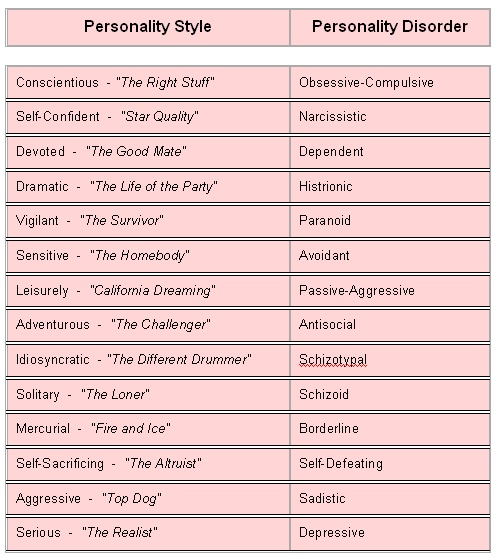
\includegraphics{assets/unit_10/U10_image.jpg}

\emph{image of chart listing of personality style and personality disorder}

\textbf{\emph{This is not to say that psychological diagnoses have no validity. The point is that diagnosis is difficult and sometimes controversial.}}

\subsection*{Activity: Read and Reflect}\label{activity-read-and-reflect-15}
\addcontentsline{toc}{subsection}{Activity: Read and Reflect}

\begin{reflect}
The following articles augment your understanding of the descriptions of the disorders discussed in the textbook and provide opportunity to understand more about anxiety disorders. Due to the pervasiveness of disorders, especially anxiety related problems, this information could prove invaluable in helping yourself and others find hope and help in challenging circumstances. There is also an excellent write up on the many valid criticisms of being overly dependent on the DSM as a resource.

\begin{itemize}
\tightlist
\item
  \href{https://psychologyinfo.com/}{\textbf{Psychological Problems and Disorders}}\\
\item
  \href{https://psychologyinfo.com/}{\textbf{Anxiety Disorders}}\\
\item
  \href{https://www.pchtreatment.com/dsm-5-issues/}{\textbf{Criticism of America's Diagnostic Bible- The DSM}}
\end{itemize}
\end{reflect}

\subsection*{Activity: Questions for Consideration}\label{activity-questions-for-consideration-16}
\addcontentsline{toc}{subsection}{Activity: Questions for Consideration}

\begin{reflect}
Consider what you have learned in this section. Use the following questions to guide your reflection:

\begin{itemize}
\tightlist
\item
  \textbf{\emph{Would you expect Christians to be more mentally healthy than non-Christians? Why or why not?}}\\
\item
  \textbf{\emph{What about people with other religious/spiritual beliefs?}}\\
\item
  \textbf{\emph{What about people with no religious/spiritual beliefs?}}
\end{itemize}

\emph{Be prepared to share your thoughts and insights with other members of the class}
\end{reflect}

\section{Mood Disorders}\label{mood-disorders}

Before we consider mood disorders, take moment to read through the following case:

\emph{Jane (not her real name) was a married church-going woman. She seemed to live a normal, uneventful life. Her family, however, was living a private hell. At times, Jane would be so depressed that she didn't want to get out of bed. She would mope around the house. She didn't want to see anyone or visit anyone. Her children and husband tried to lift her spirits, but their efforts were all in vain. She believed she was worthless, useless, and her life was meaningless. At other times, Jane was the life of the party. She would make great plans to change the world. She would give huge sums of money to charity and she would go on pointless, spending frenzies. Her husband was forced to cancel their credit cards for fear of personal bankruptcy. When Jane found out about the cards being cancelled she reacted violently. She told her husband that he was old, ugly and worthless, and that she could be with anyone she wanted. In fact, she stated that all the young men are staring at her---``If I wasn't a committed Christian, I'd be leave you to be with one of those young men, they all want me.'' Her family could no longer stand Jane's mood swings---she was either ``pathetic'' or ``unbearable''. After years of mood fluctuations, Jane was finally diagnosed as suffering from Bipolar Mood Disorder. Following medical treatment and counselling, Jane's moods stabilized and the family was again able to live peacefully.}

\section{Depression}\label{depression}

Depression is one of the most common psychological problems of all---striking Christians and non-Christians alike. Mental health workers sometimes refer to it as ``the common cold'' of psychological disorders.

In depression we once again see the link between normal and abnormal behavior. We all feel sad or down sometimes. A diagnosis of depression, however, is an extreme and continuing sadness. You will see more about the criteria for this diagnosis in the textbook and the online resources.

\section{Heartsick}\label{heartsick}

*Depression Hurts the Heart

Experts have long thought depression could be bad for your heart. A new study demonstrates just how dangerous it can be. Brenda Penninx, a gerontologist at Wake Forest University in Winston-Salem, N.C., and colleagues followed 2,847 people over 55---both with and without heart disease---for four years to trace the effects of depression.

In the end, people with major depression were at least three times as likely as patients who were not depressed to die of heart disease. Even subjects with mild depression experienced a fatality rate that was 50 percent higher than normal.

\emph{Penninx isn't sure exactly what the connection is, but since depression can raise stress, and stress triggers an outpouring of the hormone cortisol, this could cause heart rate and blood pressure to rise. Other factors could play a part: Depressed people are less likely to exercise or eat right than those who don't suffer from the malady. ``Depression deserves a lot more attention than it usually gets,'' Penninx warns. ``It's a huge cardiac risk factor, so it's crucial to take care of your emotions.''``} ---Health (Quoted in Readers Digest, Feb.~2002, p.~27)*

\subsection*{Activity: Read and Reflect}\label{activity-read-and-reflect-16}
\addcontentsline{toc}{subsection}{Activity: Read and Reflect}

\begin{reflect}
How do you know the difference between depression and normal sadness? In this activity, you are given an overview of depression that explains the causes, describes the diagnostic criteria, and offers some treatment options. Additionally, though children may suffer from a disorder, there are additional challenges in noticing it in them due to their immature language, cognitive, and emotion processing abilities and developmental stage. The second resource provides an overview of recognizing the signs that a child is struggling due to a disorder.

\begin{itemize}
\tightlist
\item
  \href{https://psychologyinfo.com/}{\textbf{Information about Depression}}\\
\item
  \href{https://www.mayoclinic.org/healthy-lifestyle/childrens-health/in-depth/mental-illness-in-children/art-20046577}{\textbf{Mental Illness in Children}}
\end{itemize}
\end{reflect}

\subsection*{Activity: Questions for Consideration}\label{activity-questions-for-consideration-17}
\addcontentsline{toc}{subsection}{Activity: Questions for Consideration}

\begin{reflect}
Consider the how the following questions relate to what you have learned in this section:

\begin{itemize}
\tightlist
\item
  \textbf{\emph{Can you think of some examples of biblical characters that apparently suffered from a mood disorder? Describe their behavior?}}\\
\item
  \textbf{\emph{What do their examples suggest about possible causes? (Hint: Elijah, David, Saul, others?)}}
\end{itemize}

\emph{If you are not familiar with biblical personages, give an example from literature or contemporary public life.}

\emph{Be prepared to share your thoughts with other members of the class}
\end{reflect}

\section{Schizophrenia}\label{schizophrenia}

Schizophrenia is one of the more devastating psychological illnesses. Schizophrenia is not common, however, it seems to be universal, appearing in cultures all over the world and across history. Some of our earliest writings describe people who seem to have lost touch with reality, who ``hear voices,'' and who produce bizarre speech and behaviours. At some earlier times in history, a person experiencing such symptoms may have been suspected of demon possession or some form of witchcraft. At other times and places, such people might be revered as shamans or as having special connections to the spirit world, and may well have played important roles in the community. Importantly, spiritual contributions to schizophrenia's symptoms are still considered in some religious and cultural interpretations of this disorder.

\subsection*{Schizophrenia in the Bible}\label{schizophrenia-in-the-bible}
\addcontentsline{toc}{subsection}{Schizophrenia in the Bible}

\emph{But when his heart was lifted up, and his mind hardened in pride, he was deposed from his kingly throne, and they took his glory from him. And he was driven from the sons of men, and his heart was made like the beasts, and his dwelling was with the wild asses; they fed him with grass like oxen, and his body was wet with the dew of heaven, till he knew that the Most High God ruled in the kingdom of men, and that he appointeth over it whomsoever he will.} Daniel 5:20-21

The bible gives relatively few accounts of people troubled by mental illness as we would call it today. The above account is of Belshazar, son of Nebuchadnezzar who was killed after losing his mental faculties. Interestingly, his father, Nebuchadnezzzar seemed to suffer from a similar loss of functioning:

\emph{O King Nebuchadnezzar, to thee it is spoken, The kingdom is departed from thee. And they shall drive thee from men, and thy dwelling shall be with the beasts of the field; they shall make thee to eat grass like oxen, and seven times shall pass over thee, until thou know that the Most High ruleth in the kngdom of men, and giveth it to whomsoever he will. The same hour was the thing fulfilled upon Nebuchadnezzar, and he was driven from men, and did eat grass like oxen, and his body was wet with the dew of heaven, till his hairs were grown like eagles' feathers, and his nails like birds' claws.} Daniel, 4:31b-33

\subsection*{The Split in Schizophrenia}\label{the-split-in-schizophrenia}
\addcontentsline{toc}{subsection}{The Split in Schizophrenia}

This strange behavior and apparent loss of contact with reality we would probably consider schizophrenia today. Schizophrenia appears in all cultures at about the same rate. Schizophrenia is one of the most serious and debilitating of the psychological disorders. As mentioned in the textbook, schizophrenia is often confused with dissociative identity disorder (multiple personality disorder, popularly known as split personality). \textbf{\emph{Schizophrenics do not have a split personality. And it is not correct to refer to someone with a ``split personality'' as schizophrenic.}} The ``split'' (schism) that schizophrenics experience is a split from reality. Schizophrenics may suffer from disorganized thought, paranoid delusions, hallucinations, and many other unusual thought patterns.

\subsection*{Activity: Read and Reflect}\label{activity-read-and-reflect-17}
\addcontentsline{toc}{subsection}{Activity: Read and Reflect}

\begin{reflect}
Schizophrenia is a truly fascinating condition that continues to draw much attention. This activity presents current in-depth research and general information concerning schizophrenia that will illuminate the complexity of the development and treatment of this disorder.

\begin{itemize}
\tightlist
\item
  \href{http://schizophrenia.com/}{\textbf{Schizophrenia}}
\end{itemize}
\end{reflect}

\subsection*{Activity: Question for Consideration}\label{activity-question-for-consideration-6}
\addcontentsline{toc}{subsection}{Activity: Question for Consideration}

\begin{reflect}
Take a moment to reflec on what you have learned using the question below:

\begin{itemize}
\tightlist
\item
  \textbf{\emph{Before the development of modern psychology, how do you think people suffering from schizophrenia were treated? How much better is treatment today?}}
\end{itemize}

\emph{Be prepared to share your thoughts and insights with other members of the class.}
\end{reflect}

\section{Personality Disorders}\label{personality-disorders}

Personality disorders are relatively common disorders where the person can function normally, but shows evidence of some difficulty or abnormality in social functioning. Unlike other disorders, the person does not seem to feel there is a difficulty.

\subsection*{Antisocial Personality}\label{antisocial-personality}
\addcontentsline{toc}{subsection}{Antisocial Personality}

Antisocial Personality Disorder (APD) is a pattern of disregard for, and violation of, the rights of others. It can be seen in individuals who have a profound lack of empathy or emotional connection with others, a disregard for others' rights or preferences, and a tendency toward imposing their own desires, often violently, onto others regardless of the consequences for other people or, often when younger, other animals. APD (sometimes referred to as psychopathy) tends to be highly resistant to treatment, in part because individuals with APD are not alarmed or distressed by their actions (although others frequently are), and they are thus rarely, if ever, motivated to change. The following is a short example to illustrate how some people who suffer from APD might present themselves:

A former professor at UBC, Dr.~Robert Hare (an internationally known expert on antisocial personality disorders) often conducted research with prisoners diagnosed with antisocial personality disorder. He frequently took graduate students with him to prison to assist in this research. To illustrate the ability of the prisoners to ``con'' even bright graduate students, he told them that on the way back from prison inevitably the students would tell him that the prisoner they had been dealing with was innocent. They were sure there had been a mistake, and the prisoner had been falsely convicted. Such is the charm and persuasive power of the antisocial personality.

\subsection*{Activity: Read and Reflect}\label{activity-read-and-reflect-18}
\addcontentsline{toc}{subsection}{Activity: Read and Reflect}

\begin{reflect}
Recall from Chapter 12 that our personalities allow others to predict and anticipate our responses to situations. A person with a ``healthy'' personality demonstrates a range of coping responses and styles when placed in a stressful situation. However, a disordered personality does not have this kind of adaptability and flexibility. At times, the person doesn't feel they like they have any problems, at other times, the lack of adaptability and the limited repertoire of coping responses can result in distress for the person and for those around him or her. In this activity, you can gain more insight into defined patterns of personality disorders.

\begin{itemize}
\tightlist
\item
  \href{https://www.camh.ca/en/health-info/mental-illness-and-addiction-index/personality-disorders}{\textbf{Personality Disorders}}
\end{itemize}
\end{reflect}

\subsection*{Activity: Chapter 15 Key Terms Quiz}\label{activity-chapter-15-key-terms-quiz}
\addcontentsline{toc}{subsection}{Activity: Chapter 15 Key Terms Quiz}

\begin{reflect}
In order to review some of the major terms from Chapter 15 in your textbook, take the following unmarked quiz. Although you will not be evaluated on these terms, they will assist you in the assessments for this course.
\end{reflect}

\subsection*{Activity: Questions for Consideration}\label{activity-questions-for-consideration-18}
\addcontentsline{toc}{subsection}{Activity: Questions for Consideration}

\begin{reflect}
\begin{itemize}
\tightlist
\item
  \textbf{\emph{Do you ever wonder if someone you know seems to have a personality disorder? What are some indications that you have seen that make you curious if there may be a problem? (If you don't know anyone personally, you can describe someone you know about or have seen in a movie/TV show.)}}
\end{itemize}

\emph{Be prepared to share your thoughts with other members of the class}
\end{reflect}

\section*{Assessment}\label{assessment-9}
\addcontentsline{toc}{section}{Assessment}

\begin{assessment}
Refer to the course schedule for graded assignments you are responsible for submitting. \textbf{All graded assignments, and their due dates, can be found on the ``Assessment'' tab.}

In addition to any graded assignments you are responsible for submitting, be sure to complete all the Learning Activities that have been provided throughout the content - these are intended to support your understanding of the content.
\end{assessment}

\section*{Checking your Learning}\label{checking-your-learning-9}
\addcontentsline{toc}{section}{Checking your Learning}

\begin{progress}
Before you move on to the next unit, check that you are able to:

\begin{itemize}
\item
  Define the key terminology associated with defining and classifying psychological disorders, personality and dissociative disorders, anxiety, obsessive-compulsive, and depressive disorders, and schizophrenia.
\item
  Describe advantages and criticisms associated with the Diagnostic and Statistical Manual of Mental Disorders (DSM-5).
\item
  Apply your knowledge of the mental disorders defense to decide if defendants are criminally responsible for their actions.
\item
  Analyze whether the benefits of labelling psychological disorders outweigh the disadvantages, the status of dissociative identity disorder as a legitimate diagnosis, and whether maladaptive aspects of specific phobias might arise from perfectly normal, healthy behaviours.
\item
  Apply your knowledge of antisocial personality disorder to explain how it could help people succeed in certain professions.
\item
  Describe the different types of anxiety disorders and how anxiety or depressive disorders can be self-perpetuating.
\item
  Apply your knowledge of anxiety, obsessive-compulsive, and depressive disorders, to be alert to people who might benefit from some help, and to be able to identify different forms of schizophrenia.
\item
  Describe how different neurotransmitters affect individuals with schizophrenia and the genetic and environmental contributions to this disorder.
\item
  Analyze claims that schizophrenia is related to genius or violent behaviour.
\end{itemize}
\end{progress}

\chapter{Therapy- Part 1}\label{therapy--part-1}

\section*{Overview}\label{overview-10}
\addcontentsline{toc}{section}{Overview}

Units 11 and 12 introduce the exciting, and ever expanding, world of therapy. Today, psychotherapeutic techniques are used to address a range of human conditions- from helping people find hope in overwhelmingly challenging circumstances to people exploring ways to optimize their potentials. Having a therapeutic relationship can be tremendously valuable in a person's life as a therapist should be non-judgmental and have no other agenda than to help a person reach their therapeutic goals. The focus of this unit will be to provide some overview and perspectives on therapy.

\subsection*{Topics}\label{topics-10}
\addcontentsline{toc}{subsection}{Topics}

This unit is will delve into the topic of :

\begin{itemize}
\tightlist
\item
  Therapies
\end{itemize}

\subsection*{Learning Outcomes}\label{learning-outcomes-10}
\addcontentsline{toc}{subsection}{Learning Outcomes}

By the end of this unit, student's will be able to:

\begin{itemize}
\tightlist
\item
  Define the key terminology associated with mental health treatment, psychological therapies, and biological treatments.\\
\item
  Describe the major barriers to seeking help for psychological disorders, arguments for and against involuntary treatment, and general approaches to conducting major types of psychotherapy.\\
\item
  Apply your knowledge to suggest what approach to therapy is likely most appropriate for a given situation, to identify major therapeutic techniques, and which drug therapies could be used for different psychological conditions.\\
\item
  Analyze whether self-help options, such as popular books, are a useful therapy option, the pros and cons of the major types of psychotherapy and whether St.~John's Wort, a popular herbal remedy for depression, works.\\
\item
  Describe how the drugs described in this module, and the other major medical approaches to therapy, affect brain functioning.
\end{itemize}

\subsection*{Activity Checklist:}\label{activity-checklist-10}
\addcontentsline{toc}{subsection}{Activity Checklist:}

Here is a checklist of learning activities you will benefit from in completing this unit. You may find it useful for planning your work.

\begin{reflect}
{Learning Activities}

\begin{itemize}
\tightlist
\item
  Read the relevant sections of Chapter 16 of your textbook
\item
  Review the Chapter 16 - Notes (intended to support your understanding of your readings)
\item
  Read and reflect about the articles from \emph{PsychCentral,} \emph{Behaviour Online,} and \emph{Integration Models}
\end{itemize}
\end{reflect}

\begin{caution}
\textbf{\emph{Note}}

The course units follow topics in the textbook, \emph{Revel for An Introduction to Psychological Science} by Krause et al.~(4th Edition). For each unit, please read the pertinent chapter(s) before completing the assessment for the unit.
\end{caution}

\begin{assessment}
\textbf{\emph{Assessment}}

In this course you demonstrate your understanding of the course learning outcomes in different ways, including papers, projects, discussions and quizzes. Please see the Assessment section in Moodle for assignment details and due dates.
\end{assessment}

\subsection*{Resources}\label{resources-10}
\addcontentsline{toc}{subsection}{Resources}

Here are the resources you will need to complete this unit:

\begin{itemize}
\tightlist
\item
  Krause, M., Corts, D., \& Smith, S. C. (2024). \emph{Revel for An Introduction to Psychological Science, 4th Canadian Edition.} Pearson Ed.
\item
  Other resources will be provided online.
\end{itemize}

\section{Therapies- Part 1}\label{therapies--part-1}

\subsection*{Psychological Therapies}\label{psychological-therapies}
\addcontentsline{toc}{subsection}{Psychological Therapies}

Psychological therapies, or psychotherapies, are a general class of therapies that deal with the psychological (mental/behavioural) world of people with disorders.

These therapies are generally contrasted with biomedical approaches, which deal more with the biological world of the individual. Biomedical therapies focus on altering a person's biology to effect a change in the person's psychology.

\subsection*{Eclectic Approach}\label{eclectic-approach}
\addcontentsline{toc}{subsection}{Eclectic Approach}

The eclectic approach is an approach that values the diversity of treatment approaches. Eclectic approaches deal with psychology and biology. In addition, various types of psychotherapies may be employed. Eclectic therapy approaches are becoming very popular.

\subsection*{A Sin Problem?}\label{a-sin-problem}
\addcontentsline{toc}{subsection}{A Sin Problem?}

*``Many Christians are not satisfied with viewing psychological disorders as either illnesses or nothing but thought and behavior problems. They feel that both of these approaches are inadequate because they omit very important moral and spiritual questions. Consequently, the important issue of moral responsibility is not dealt with adequately.

They feel that since humanity's most basic problem is alienation from God as a result of sin, no other difficulty can be dealt with until the relationship with God has been restored. Thus the first goal of therapy is to bring the client to the place of acknowledging his or her need, and asking for divine forgiveness through Jesus Christ. Once the client has placed his or her trust in God, and is operating within the same religious conceptual framework as the therapist, therapy can then proceed to the identification of specific disturbances of thought and behavior. These are seen as examples of sin in that the individual is either acting in a sinful way towards others, or is harboring sinful thoughts and attitudes within. The therapist will assist the individual to identify, confess, and forsake these sins. The goal of therapy is seen primarily in terms of spiritual growth and a ``closer walk with God.''*

\subsection*{Sin Only?}\label{sin-only}
\addcontentsline{toc}{subsection}{Sin Only?}

In a work for Christian counselors, Koteskey (1983) gives the example of his eighteen month old son who developed an intense fear of dogs after two unpleasant experiences with them. Even the fact that the child was too young to talk did not prevent a fellow Christian psychologist from concluding that he had a spiritual problem. We should recognize that not every problem is necessarily a spiritual one. Just as a disturbance may have a purely biological cause, so too it may have a simple psychological (learning) explanation. Information gained from the study of animals may be helpful in the understanding of psychological problems as it is often vital in understanding biological problems. \emph{(Both excerpts from Psychology and Christianity by Ronald Philipchalk)}

\subsection*{Activity: Read and Reflect}\label{activity-read-and-reflect-19}
\addcontentsline{toc}{subsection}{Activity: Read and Reflect}

\begin{reflect}
For many people unfamiliar with the journey of counselling, finding suitable resources may feel daunting. It is important to know that there are many different approaches designed to help you accomplish the growth goals you have for your life. In this activity, the first resource, Psych Central is the oldest peer-reviewed psychology and mental health network on the Internet. Established in 1992, originally it was an index to mental health. Now it gives you the opportunity to see some treatment options for a wide variety of conditions. Additionally, there is a resource on different theoretical approaches to behavior change, and a link to some information concerning the integration of Christianity and psychotherapy.

\begin{itemize}
\item
  \href{https://psychcentral.com/}{\textbf{PsychCentral}}
\item
  \href{http://www.behavior.net}{\textbf{Behaviour Online}}
\item
  \href{http://www.psyche.gr/lpsycrel.htm}{\textbf{Integration Models}}
\end{itemize}
\end{reflect}

\subsection*{Activity: Questions for Consideration}\label{activity-questions-for-consideration-19}
\addcontentsline{toc}{subsection}{Activity: Questions for Consideration}

\begin{reflect}
Read the questions below and consider how they connect to what you have learned:

\begin{itemize}
\tightlist
\item
  \textbf{\emph{What is your view of the role of sin (or questionable moral behaviours) or other religious/spiritual beliefs in the treatment of psychological disorders?}}\\
\item
  \textbf{\emph{What kinds of religious/spiritual beliefs could lead to greater feelings of guilt/shame and increased psychological disorder?}}
\end{itemize}

\emph{Be prepared to share your thoughts with other members of the class.}
\end{reflect}

\section*{Assessment}\label{assessment-10}
\addcontentsline{toc}{section}{Assessment}

\begin{assessment}
Refer to the course schedule for graded assignments you are responsible for submitting. \textbf{All graded assignments, and their due dates, can be found on the ``Assessment'' tab.}

In addition to any graded assignments you are responsible for submitting, be sure to complete all the Learning Activities that have been provided throughout the content - these are intended to support your understanding of the content.
\end{assessment}

\section*{Checking your Learning}\label{checking-your-learning-10}
\addcontentsline{toc}{section}{Checking your Learning}

\begin{progress}
Before you move on to the next unit, check that you are able to:

\begin{itemize}
\item
  Define the key terminology related to health psychology, stress and illness, and coping and well-being.
\item
  Describe how genetic and environmental factors influence obesity, how physiological reactions that occur under stress, and how the immune system is connected to stress responses.
\item
  Apply your knowledge of persuasion and health to examine the effectiveness of different types of cigarette warnings, and of the beneficial effects of optimism to help you reframe stressful situations as positive opportunities.
\item
  Analyze whether media depictions of smoking affect smoking in adolescents, the claim that ulcers are caused by stress, and whether activities such as relaxation techniques, meditation, and biofeedback actually help people cope with stress and problems.
\item
  Describe how control over the environment and positive and negative styles of coping influences well-being.
\end{itemize}
\end{progress}

\chapter{Therapy - Part 2}\label{therapy---part-2}

\section*{Overview}\label{overview-11}
\addcontentsline{toc}{section}{Overview}

Our final unit expands upon Unit 11 and introduces the exciting, and ever expanding, world of therapy. Today, psychotherapeutic techniques are used to address a range of human conditions, from helping people find hope in overwhelmingly challenging circumstances to people exploring ways to optimize their potentials. Having a therapeutic relationship can be tremendously valuable in a person's life as a therapist should be non-judgmental and have no other agenda than to help a person reach their therapeutic goals. This final unit of the course will continue to build upon Unit 11 by discussing the effectiveness of therapy, some of the biological treatment options, and some tips on preventing problems.

\subsection*{Topics}\label{topics-11}
\addcontentsline{toc}{subsection}{Topics}

This unit will be divided into the following topics:

\begin{enumerate}
\def\labelenumi{\arabic{enumi}.}
\tightlist
\item
  Evaluating Therapy\\
\item
  Biological Treatments\\
\item
  Preventing Problems
\end{enumerate}

\subsection*{Learning Outcomes}\label{learning-outcomes-11}
\addcontentsline{toc}{subsection}{Learning Outcomes}

By the end of this unit, student's will be able to:

\begin{itemize}
\tightlist
\item
  Define the key terminology associated with mental health treatment, psychological therapies, and biological treatments.\\
\item
  Describe the major barriers to seeking help for psychological disorders, arguments for and against involuntary treatment, and general approaches to conducting major types of psychotherapy.\\
\item
  Apply your knowledge to suggest what approach to therapy is likely most appropriate for a given situation, to identify major therapeutic techniques, and which drug therapies could be used for different psychological conditions.\\
\item
  Analyze whether self-help options, such as popular books, are a useful therapy option, the pros and cons of the major types of psychotherapy and whether St.~John's Wort, a popular herbal remedy for depression, works.\\
\item
  Describe how the drugs described in this module, and the other major medical approaches to therapy, affect brain functioning.
\end{itemize}

\subsection*{Activity Checklist:}\label{activity-checklist-11}
\addcontentsline{toc}{subsection}{Activity Checklist:}

Here is a checklist of learning activities you will benefit from in completing this unit. You may find it useful for planning your work.

\begin{reflect}
{Learning Activities}

\begin{itemize}
\tightlist
\item
  Read the relevant sections of Chapter 16 of your textbook
\item
  Review Chapter 16 - Notes (intended to support your understanding of your readings)
\item
  Read and reflect about the section from the \emph{American Psychological Association}
\item
  Read and reflect about the articles \emph{Electroconvulsive Therapy and Other Depression Treatments} and \emph{International Society for Neuroregulation and Research}
\item
  Read and reflect about the articles \emph{Psychology Help Center,} \emph{How to Choose a Therapist,} and \emph{Rights and Responsibilities in Psychotherapy}
\end{itemize}
\end{reflect}

\begin{caution}
\textbf{\emph{Note}}

The course units follow topics in the textbook, \emph{Revel for An Introduction to Psychological Science} by Krause et al.~(4th Edition). For each unit, please read the pertinent chapter(s) before completing the assessment for the unit.
\end{caution}

\begin{assessment}
\textbf{\emph{Assessment}}

In this course you demonstrate your understanding of the course learning outcomes in different ways, including papers, projects, discussions and quizzes. Please see the Assessment section in Moodle for assignment details and due dates.
\end{assessment}

\subsection*{Resources}\label{resources-11}
\addcontentsline{toc}{subsection}{Resources}

Here are the resources you will need to complete this unit:

\begin{itemize}
\tightlist
\item
  Krause, M., Corts, D., \& Smith, S. C. (2024). \emph{Revel for An Introduction to Psychological Science, 4th Canadian Edition.} Pearson Ed.\\
\item
  Other resources will be provided online.
\end{itemize}

\section{Evaluating Therapy}\label{evaluating-therapy}

\subsection*{Therapy?}\label{therapy}
\addcontentsline{toc}{subsection}{Therapy?}

In a previous chapter, we looked at various ways of understanding personality. In the first part of this chapter we have been considering different therapies that grow out of these personality theories. Now it is time to ask the question, ``Does it work? Is psychotherapy effective?'' The answer seems to be ``Yes,'' but there are qualifications. First, many people who do not receive treatment get better anyway. And second, placebo treatments also produce improvements, as do non-professional caring relationships. As David Myers says,

\emph{``All types of psychotherapy seem to offer three benefits: new hope, a fresh perspective, and an empathic, trusting, caring relationship.'' (p.~592)}

When you stop and think about it, isn't this what a good friend offers? Maybe if we all experienced (and offered) this kind of friendship, therapists wouldn't be so much in demand.

\subsection*{Therapy in Other Cultures}\label{therapy-in-other-cultures}
\addcontentsline{toc}{subsection}{Therapy in Other Cultures}

The process of psychotherapy generally assumes a cultural value of sharing your inner feelings and problems with another individual. David Ho observes that in the culture of Hong Kong, it is a sign of weakness to talk about one's problems and to reveal much of one's self. This cultural background influences the style of therapy and the process of psychotherapy. How would you proceed if you were a therapist?

Paul Pedersen (1985; 1987; 2000) suggests that we do not need to look at cultures outside North America to see differences in the process of psychotherapy. He sug­gests that different sub cultural minorities within North America approach psy­chotherapy with different values and different expectations. Native North American cultures, Asian immigrants, Hispanics, and Afro-Americans have different approaches to the pro­cess of psychotherapy. A therapist needs to be aware of these cultural differ­ences to perform effectively in the therapeutic situation.

\subsection*{Activity: Read and Reflect}\label{activity-read-and-reflect-20}
\addcontentsline{toc}{subsection}{Activity: Read and Reflect}

\begin{reflect}
As mentioned earlier, this activity gives you an opportunity to explore the American Psychological Association (APA) website. In many ways, the APA leads the discipline and profession of psychology. It is an excellent resource for finding information on a number of areas of psychology, contemporary issues in psychology, a plethora of resources for self-help. They also have the opportunity for students to become student affiliates and enjoy member privileges that will contribute to your development as a professional. Follow the link below:

\begin{itemize}
\tightlist
\item
  \href{https://www.apa.org/}{\textbf{American Psychological Association}}
\end{itemize}
\end{reflect}

\subsection*{Activity: Question for Consideration}\label{activity-question-for-consideration-7}
\addcontentsline{toc}{subsection}{Activity: Question for Consideration}

\begin{reflect}
Consider the following:

\begin{itemize}
\tightlist
\item
  \textbf{\emph{Do you think an empathic, trusting, caring friend could be as effective as a trained psychotherapist or counselor?}}
\end{itemize}

\emph{Be prepared to share your thoughts and insights with other members of the class}
\end{reflect}

\section{Biological Treatments}\label{biological-treatments}

Though there are a number of treatments options within the field of psychology, there are two basic treatment models:

\begin{enumerate}
\def\labelenumi{\arabic{enumi}.}
\tightlist
\item
  The Wellness Model\\
\item
  The Medical Model.
\end{enumerate}

The Wellness Model will look intently, and holistically, at a number of areas of a person's life (thoughts/emotions, relationships, work/academics, developmental stage, nutrition, activity/leisure, and sleep, to name a few) and illuminate the client's strengths and resources to help them find a way to overcome challenges and lead a more fulfilling life. Many of the psychotherapeutic approaches looked at, thus far, operate on this model.

The Medical Model, however, is based on symptom recognition, (differential) diagnosis, prognosis, and often a pharmacological support and possibly an invasive or non-invasive procedure. The topic of biological treatments is based on the medical model.

\subsection*{Medical Treatments}\label{medical-treatments}
\addcontentsline{toc}{subsection}{Medical Treatments}

Although psychotherapy in its various forms has grown in importance over the past generation, people are still more inclined to seek the help of medical professionals over mental health professionals for their psychological concerns. One of the greatest changes in the way we have treated psychological disorders has been through the discovery and use of various drugs. In this section, we consider the various biomedical therapies that are available for psychological disorders.

\subsection*{Not a Panacea}\label{not-a-panacea}
\addcontentsline{toc}{subsection}{Not a Panacea}

All of the biological therapies produce side effects, some of them permanent. Since the brain cannot regenerate itself, psychosurgery is irreversible; ECT destroys brain cells, producing memory loss, some of which is permanent; virtually all drugs have side effects besides the dependency produced, and some of these are permanent. (For example, one class of antipsychotic drugs, the phenothiazines, can produce a permanent and irreversible muscle disorder, particularly after massive long-term use. This disorder, called tardive dyskinesia, is evidenced by involuntary movements of the face, limbs, and trunk.) Furthermore, the unknown basis of the effects of many of these techniques (e.g., ECT, and some drugs), and the exploratory nature of others (psychosurgery) should make us at least a little skeptical. (A further controversy surrounding the use of physiological therapies, particularly, ECT, concerns their forced administration to involuntary patients.)

\subsection*{Activity: Read and Reflect}\label{activity-read-and-reflect-21}
\addcontentsline{toc}{subsection}{Activity: Read and Reflect}

\begin{reflect}
It is important, when considering biological treatments, to receive input from more than one professional and to do adequate research on the treatment to understand the potential risks and benefits. This activity serves as a resource for electroconvulsive therapy (ECT), transcranial magnetic stimulation (TMS), and vagus nerve stimulation (VNS) as treatments for depression. It also has a link to explore an alternative therapy known as neurotherapy/neurofeedback, which is a safe (when administered by a well-trained professional), non-invasive option for a number of different developmental and psychological matters. To learn more, read below:

\begin{itemize}
\tightlist
\item
  \href{https://www.camh.ca/en/health-info/mental-illness-and-addiction-index/electroconvulsive-therapy}{\textbf{Electroconvulsive Therapy and Other Depression Treatments}}
\item
  \href{https://isnr.org/}{\textbf{International Society for Neuroregulation and Research}}
\end{itemize}
\end{reflect}

\subsection*{Activity: Read and Reflect}\label{activity-read-and-reflect-22}
\addcontentsline{toc}{subsection}{Activity: Read and Reflect}

\begin{reflect}
Consider the following questions in context of what you have learned about in this section:

\begin{itemize}
\tightlist
\item
  \textbf{\emph{As biological influence in psychological disorders becomes more obvious, what are the implications for psychologists and ``talk therapy?''}}
\item
  \textbf{\emph{Will biological therapies eventually replace old style talk therapies?}}
\end{itemize}

\emph{Be prepared to share your thoughts with other members of the class}
\end{reflect}

\section{Preventing Problems}\label{preventing-problems}

\textbf{\emph{A Little Help When You Need It\ldots{}}}

The textbook discusses the value of prevention on a broad level, including environmental changes. Here, we take a more personal look at how you might go about dealing with major problems or just simple blockages in your pathway to growth.

We all need help from time to time, whether we get it from family, friends, or paid professionals. Professional help can be a real boost. It might be testing to clarify career directions, sharing a relationship issue with a sympathetic listener, or in-depth study of a long-term problem. A trained helper provides an objective perspective and an empathic ear.

\subsection*{An Ounce of Prevention}\label{an-ounce-of-prevention}
\addcontentsline{toc}{subsection}{An Ounce of Prevention}

Being aware of the possible causes of psychological problems as well as the appropriate treatments can help you avoid similar difficulties in your own life. For example you can:

\begin{itemize}
\tightlist
\item
  Not bury and deny strong emotions (psychodynamic view)\\
\item
  Take responsibility for your feelings \& promote growth (humanistic view)\\
\item
  Associate positive consequences with desirable actions and negative results with undesirable ones (behavioral view)\\
\item
  Avoid negative self-talk in favor of positive (cognitive view)\\
\item
  Cultivate empathic, trusting, caring relationships\\
\item
  Take steps to ensure a healthy body
\end{itemize}

\subsection*{Activity: Read and Reflect}\label{activity-read-and-reflect-23}
\addcontentsline{toc}{subsection}{Activity: Read and Reflect}

\begin{reflect}
Looking intently at how you are spending your time and taking preventative steps to contribute to your mental/emotional health and overall well-being is a great gift to give to yourself (and ultimately others). This activity offers a resource where you can find information on a variety of (usually research-based) preventative strategies. Moreover, if you decide that you would like to explore therapy for yourself, there are resources here to inform you as to how to find a suitable therapist and what some of your rights and responsibilities are in therapy.

\begin{itemize}
\tightlist
\item
  \href{https://www.apa.org/helpcenter/}{\textbf{Psychology Help Center}}\\
\item
  \href{http://psychcentral.com/therapst.htm}{\textbf{How to Choose a Therapist}}\\
\item
  \href{https://psychcentral.com/blog/your-patient-rights-in-therapy\#1}{\textbf{Rights and Responsibilities in Psychotherapy}}
\end{itemize}
\end{reflect}

\subsection*{Activity: Questions for Consideration}\label{activity-questions-for-consideration-20}
\addcontentsline{toc}{subsection}{Activity: Questions for Consideration}

\begin{reflect}
Consider the following questions:

\begin{itemize}
\tightlist
\item
  \textbf{\emph{What role do your religious or other beliefs play in your efforts to avoid psychological difficulties and promote growth?}}
\item
  \textbf{\emph{Do your beliefs affect your choice of the kind of help you would look for?}}
\end{itemize}

\emph{Be prepared to share your thoughts and insights with other members of the class}
\end{reflect}

\section*{Assessment}\label{assessment-11}
\addcontentsline{toc}{section}{Assessment}

\begin{assessment}
Refer to the course schedule for graded assignments you are responsible for submitting. \textbf{All graded assignments, and their due dates, can be found on the ``Assessment'' tab.}

In addition to any graded assignments you are responsible for submitting, be sure to complete all the Learning Activities that have been provided throughout the content - these are intended to support your understanding of the content.
\end{assessment}

\section*{Checking your Learning}\label{checking-your-learning-11}
\addcontentsline{toc}{section}{Checking your Learning}

\begin{progress}
Before you move on to the next unit, check that you are able to:

\begin{itemize}
\item
  Define, and apply, the key terminology related to health psychology, stress and illness, and coping and well-being.
\item
  Describe how genetic and environmental factors influence obesity, how physiological reactions that occur under stress, and how the immune system is connected to stress responses.
\item
  Apply your knowledge of persuasion and health to examine the effectiveness of different types of cigarette warnings, and of the beneficial effects of optimism to help you reframe stressful situations as positive opportunities.
\item
  Analyze whether media depictions of smoking affect smoking in adolescents, the claim that ulcers are caused by stress, and whether activities such as relaxation techniques, meditation, and biofeedback actually help people cope with stress and problems.
\item
  Describe how control over the environment and positive and negative styles of coping influences well-being.
\end{itemize}
\end{progress}

\chapter*{Course Credits}\label{course-credits}
\addcontentsline{toc}{chapter}{Course Credits}

\section*{Course Contributors}\label{course-contributors}
\addcontentsline{toc}{section}{Course Contributors}

\subsection*{Curriculum Developer}\label{curriculum-developer}
\addcontentsline{toc}{subsection}{Curriculum Developer}

\begin{center}\rule{0.5\linewidth}{0.5pt}\end{center}

\subsection*{Course Instructors}\label{course-instructors}
\addcontentsline{toc}{subsection}{Course Instructors}

\section*{Copyright \& Credits}\label{copyright-credits}
\addcontentsline{toc}{section}{Copyright \& Credits}

\textbf{Copyright © 2023 Trinity Western University. All rights reserved.}

The content of this course material is the property of Trinity Western University (TWU) and is protected by copyright law worldwide. This material may be used by students enrolled at TWU for personal study purposes only.

TWU seeks to ensure that any course content that is owned by others has been appropriately cleared for use in this course. Anyone wishing to make additional use of such third party material must obtain clearance from the copyright holder.

\subsection{Course Development Team}\label{course-development-team}

Course Writer:
Instructional Designer:
Production Team:
Department Chair:
Dean:

Trinity Western University
22500 University Drive
Langley, BC, Canada \textbar{} V2Y 1Y1

\chapter*{References}\label{references}
\addcontentsline{toc}{chapter}{References}

The following are key references used in this course. \textbf{\emph{Check with your course syllabus for required readings.}}

  \bibliography{book.bib}

\end{document}
